\documentclass[11pt,a4paper,oneside,openany,fontset=none]{ctexbook}
% ===== 丘维声《解析几何》讲解 · 统一样式（与第 1–5 批一致） =====
\usepackage[a4paper,top=2.4cm,bottom=2.4cm,left=2.5cm,right=2.5cm,headheight=15pt]{geometry}
\setCJKmainfont{Noto Serif CJK SC}[BoldFont={Noto Serif CJK SC Bold}]
\setCJKsansfont{Noto Sans CJK SC}[BoldFont={Noto Sans CJK SC Bold}]
\setCJKmonofont{Noto Sans Mono CJK SC}
\usepackage{amsmath,amssymb,amsthm,mathtools,bm,mathrsfs}
\usepackage{xcolor}
\usepackage{graphicx}
\usepackage{booktabs,tabularx,array,multirow}
\usepackage{enumitem}
\usepackage{fancyhdr}
\usepackage{titlesec}
\usepackage{caption}
\usepackage{needspace}
\usepackage{tikz}
\usetikzlibrary{calc,intersections,arrows.meta,positioning,decorations.markings,shapes.geometric,through,3d,perspective,patterns}
\usepackage{tikz-3dplot}
\usepackage[most]{tcolorbox}
\usepackage[hidelinks,bookmarksnumbered,bookmarksopen]{hyperref}

% ---------- 颜色 ----------
\definecolor{mainblue}{HTML}{1F5FA8}
\definecolor{defblue}{HTML}{2E6DB4}   \definecolor{defbg}{HTML}{EEF3FA}
\definecolor{thmred}{HTML}{B03A2E}    \definecolor{thmbg}{HTML}{FBEFEE}
\definecolor{intor}{HTML}{C8691C}     \definecolor{intbg}{HTML}{FBF4EC}
\definecolor{gdpur}{HTML}{6C4F9E}     \definecolor{gdbg}{HTML}{F4F0F9}
\definecolor{mteal}{HTML}{1E7B6E}     \definecolor{mtbg}{HTML}{EAF5F3}
\definecolor{ckgray}{HTML}{E2E2E2}    \definecolor{ckbg}{HTML}{F7F7F7}
\definecolor{exslate}{HTML}{34495E}   \definecolor{exbg}{HTML}{F4F6F8}
\definecolor{solgreen}{HTML}{2E8B57}
\definecolor{keyred}{HTML}{C0392B}
\definecolor{figblue}{HTML}{2E6DB4}   \definecolor{figred}{HTML}{C0392B}
\definecolor{figgreen}{HTML}{2E8B57}  \definecolor{figor}{HTML}{D9822B}
\definecolor{figpur}{HTML}{7D5BA6}    \definecolor{figgray}{HTML}{7F8C8D}

% ---------- 标题样式 ----------
\ctexset{
  chapter={
    name={}, number={第\arabic{chapter}章},
    format=\centering,
    nameformat=\sffamily\bfseries\Large\color{mainblue},
    titleformat=\sffamily\bfseries\Huge\color{mainblue},
    aftername=\par\vspace{0.8em},
    beforeskip=10pt, afterskip=22pt,
    aftertitle={\par\vspace{6pt}{\color{mainblue}\rule{\textwidth}{0.8pt}}},
  },
  section={
    format=\sffamily\bfseries\Large\color{mainblue}\raggedright,
    name={\S,}, number=\thechapter.\arabic{section},
    aftername=\enspace, beforeskip=18pt, afterskip=10pt,
  },
  subsection={
    format=\sffamily\bfseries\large\color{mainblue!85!black}\raggedright,
    number=\thechapter.\arabic{section}.\arabic{subsection},
    aftername=\enspace, beforeskip=12pt, afterskip=6pt,
  },
}
\setcounter{secnumdepth}{2}
\setcounter{tocdepth}{1}
\renewcommand{\thefigure}{\thechapter-\arabic{figure}}
\captionsetup{labelsep=quad,font=small,labelfont={color=black}}

% 习题详解标题（不编号，进目录与书签）
\newcommand{\xiti}[1]{%
  \vspace{8pt}\phantomsection
  \addcontentsline{toc}{section}{习题 #1 详解}%
  {\noindent\sffamily\bfseries\Large\color{mainblue}习题 #1\ 详解\par}\vspace{8pt}}
\newcommand{\zongjie}[1]{%
  \vspace{8pt}\phantomsection
  \addcontentsline{toc}{section}{#1}%
  {\noindent\sffamily\bfseries\Large\color{mainblue}#1\par}\vspace{8pt}}

% ---------- 页眉页脚 ----------
\pagestyle{fancy}
\fancyhf{}
\fancyhead[L]{\small 丘维声《解析几何》讲解}
\fancyhead[R]{\small 第\thechapter 章\quad\leftmark}
\fancyfoot[C]{\small\thepage}
\renewcommand{\headrulewidth}{0.5pt}
\renewcommand{\chaptermark}[1]{\markboth{#1}{}}
\renewcommand{\sectionmark}[1]{}
\fancypagestyle{plain}{\fancyhf{}\fancyfoot[C]{\small\thepage}\renewcommand{\headrulewidth}{0pt}}

% ---------- 彩色框 ----------
\tcbset{
  basebox/.style={enhanced,breakable,arc=2mm,boxrule=0.6pt,
    left=6pt,right=6pt,top=4pt,bottom=4pt,
    fonttitle=\sffamily\bfseries,coltitle=white,
    before skip=8pt,after skip=8pt},
}
\newtcolorbox{defbox}[1]{basebox,colframe=defblue,colback=defbg,colbacktitle=defblue,title={#1}}
\newtcolorbox{thmbox}[1]{basebox,colframe=thmred,colback=thmbg,colbacktitle=thmred,title={#1}}
\newtcolorbox{intbox}[1]{basebox,colframe=intor,colback=intbg,colbacktitle=intor,title={#1}}
\newtcolorbox{gdbox}[1]{basebox,colframe=gdpur,colback=gdbg,colbacktitle=gdpur,title={#1}}
\newtcolorbox{mtbox}[1]{basebox,colframe=mteal,colback=mtbg,colbacktitle=mteal,title={#1}}
\newtcolorbox{ckbox}[1]{basebox,colframe=ckgray,colback=ckbg,colbacktitle=ckgray,coltitle=black,title={#1}}

% 习题题干框：深色题号标签
\newtcolorbox{ex}[1]{enhanced,breakable,arc=2mm,boxrule=0.6pt,
  colframe=exslate,colback=exbg,
  left=6pt,right=6pt,top=6pt,bottom=4pt,
  attach boxed title to top left={xshift=4mm,yshift*=-\tcboxedtitleheight/2},
  boxed title style={colback=exslate,colframe=exslate,sharp corners,boxrule=0pt,left=8pt,right=8pt,top=2pt,bottom=2pt},
  fonttitle=\sffamily\bfseries,coltitle=white,
  title={#1},before skip=14pt,after skip=4pt}

\newcommand{\jie}{\noindent{\color{solgreen}\sffamily\bfseries【解】}}
\newcommand{\zheng}{\noindent{\color{solgreen}\sffamily\bfseries【证】}}
\newcommand{\fenxi}{\noindent{\color{solgreen}\sffamily\bfseries【分析】}}
\newcommand{\gd}{{\color{gdpur}\sffamily\bfseries【高代】}}
\newcommand{\ji}{{\color{intor}\sffamily\bfseries【记】}}
\newcommand{\key}[1]{\leavevmode{\color{keyred}\bfseries #1}}
\renewcommand{\qed}{\hfill$\blacksquare$}

% ---------- 数学记号 ----------
\newcommand{\R}{\mathbb{R}}
\newcommand{\C}{\mathbb{C}}
\newcommand{\pib}{\overline{\pi}_0}
\newcommand{\Sb}{\overline{S}}
\newcommand{\linf}{l_\infty}
\newcommand{\T}{^{\mathsf T}}
\newcommand{\cro}[4]{(#1,#2;#3,#4)}
\newcommand{\vv}[1]{\boldsymbol{#1}}
\newcommand{\pt}[3]{(#1,#2,#3)\T}
\newcommand{\spn}[1]{\langle #1\rangle}
\setlist{nosep,leftmargin=2em}
\setlength{\parindent}{2em}
\linespread{1.25}

\hypersetup{pdftitle={丘维声《解析几何》知识点讲解与习题详解 第6批：第七章},pdfauthor={}}
\begin{document}
\frontmatter
\begin{titlepage}
\centering
\vspace*{0.25\textheight}
{\sffamily\bfseries\huge 丘维声《解析几何》（第三版）\par}
\vspace{1.6em}
{\sffamily\bfseries\Large 知识点讲解与习题详解\par}
\vspace{1.2em}
{\sffamily\bfseries\large 第 6 批：第七章\par}
\vfill
{\large 数形结合 · 高代联动 · 空间直觉\par}
\vspace*{2cm}
\end{titlepage}
\pagestyle{plain}
\tableofcontents
\mainmatter
\pagestyle{fancy}
\setcounter{chapter}{6}
\chapter{射影平面和它的射影变换}
% ================= §7.1 射影平面，齐次坐标 =================
\begin{intbox}{本章一句话}
前六章都在“欧氏平面”里做几何。本章给平面\key{添上一条无穷远直线}：每一组平行线共有一个“无穷远点”，于是\key{任意两条直线都相交}，平行的概念消失，点与线的地位完全对称（对偶原理）。用\key{齐次坐标} $(x_1,x_2,x_3)\T$ 记点（成比例看作同一点），则
“点 = $\R^3$ 的 1 维子空间，线 = 2 维子空间”，射影变换 = 可逆 3 阶矩阵（差一个非零倍数），
\key{交比}是射影变换下唯一的“数值”不变量，二次曲线 = 三元二次型 $X\T AX=0$ 的零点集——在射影眼里，
\key{椭圆、双曲线、抛物线是同一种曲线}，区别只在它与无穷远直线交于 0、2、1 个点。
\end{intbox}

\begin{gdbox}{高代联动：本章与高等代数的对照}
\renewcommand{\arraystretch}{1.25}
\begin{tabularx}{\linewidth}{@{}>{\raggedright\arraybackslash}X>{\raggedright\arraybackslash}X@{}}
\toprule
\textbf{\sffamily 射影几何} & \textbf{\sffamily 高等代数}\\\midrule
射影平面的点 $\spn{\vv\alpha}$ & $\R^3$ 的 1 维子空间（非零向量，差一个倍数）\\
射影直线 $\spn{\vv\beta,\vv\gamma}$；方程 $\vv u\T X=0$ & 2 维子空间；齐次线性方程的解空间\\
两点 / 两线唯一确定一线 / 一点 & 维数公式 $\dim(U\cap W)=\dim U+\dim W-\dim(U+W)$\\
三点共线 $\iff$ 三阶行列式 $=0$ & 三个向量线性相关\\
两点连线、两线交点 = 叉积 & 2 个方程 3 个未知量的齐次方程组的基础解系\\
对偶原理（点 $\leftrightarrow$ 线） & 对偶空间 $V^*$：列向量 $\leftrightarrow$ 行向量\\
射影坐标系 $[A_1,A_2,A_3,E]$ & 基 + “单位点”把各基向量的比例固定\\
射影坐标变换 $\rho X=HX'$ & 基变换的过渡矩阵（再差一个数乘）\\
射影变换 $\lambda X'=AX$，$|A|\neq0$ & 可逆线性变换模去纯量：$PGL(3,\R)$\\
不动点 / 不变直线 & $A$ 的特征向量 / $A\T$ 的特征向量\\
二次曲线 $X\T AX=0$ & 三元二次型\\
极线 $\vv p\T AX=0$，配极 & 对称双线性型；非退化型诱导的同构 $V\to V^*$\\
自配极三角形 & 合同对角化 $C\T AC=\operatorname{diag}$\\
二次曲线的射影分类（5 类） & 实二次型的惯性定理（秩 + 符号差）\\
\bottomrule
\end{tabularx}
\end{gdbox}

\section{射影平面，齐次坐标}

\subsection{中心投影与扩大的欧氏平面}

\begin{defbox}{中心投影}
设 $\pi_0,\pi_1$ 是两个平面，$O$ 是不在它们上的点。把 $\pi_0$ 上的点 $P$ 对应到直线 $OP$ 与 $\pi_1$ 的交点 $P'$，称为平面 $\pi_0$ 到 $\pi_1$ 上\key{以 $O$ 为中心的中心投影}。中心投影把共线三点变成共线三点（共线关系保持），但\key{长度、角度、平行、分比都可能改变}。
\end{defbox}

航空摄影就是中心投影：地面 $\pi_0$ 上的景物经镜头 $O$ 投到底片 $\pi_1$ 上。$\pi_0,\pi_1$ 平行时它就是相似变换（第六章），不平行时就出现了新现象：

\begin{figure}[htbp]
\centering
\begin{tikzpicture}[x={(1cm,0cm)},y={(0.55cm,0.38cm)},z={(0cm,1cm)},scale=0.95,line join=round]
  % pi0 : z=0
  \fill[defbg] (-3,-0.6,0)--(6,-0.6,0)--(6,3,0)--(-3,3,0)--cycle;
  \draw[defblue] (-3,-0.6,0)--(6,-0.6,0)--(6,3,0)--(-3,3,0)--cycle;
  % pi1 : z=1.2(x-2)
  \fill[thmbg,opacity=0.85] (2,-0.6,0)--(5,-0.6,3.6)--(5,3,3.6)--(2,3,0)--cycle;
  \draw[thmred] (2,-0.6,0)--(5,-0.6,3.6)--(5,3,3.6)--(2,3,0)--cycle;
  \node[defblue] at (-2.6,-0.3,0) {$\pi_0$};
  \node[thmred] at (4.75,2.7,3.0) {$\pi_1$};
  % vanishing line x=-2 in pi0
  \draw[figor,very thick,dashed] (-2,-0.6,0)--(-2,3,0);
  \node[figor,below] at (-2,-0.6,0) {\small 没有像的点组成的直线};
  % O
  \coordinate (O) at (0.5,1,3);
  \fill (O) circle (1.5pt) node[above left] {$O$};
  % P -> P'
  \coordinate (P) at (5,1.5,0); \coordinate (Pp) at (3.071,1.286,1.286);
  \draw[thick] (O)--(P);
  \fill (P) circle (1.5pt) node[below right] {$P$};
  \fill[thmred] (Pp) circle (1.5pt) node[above right] {$P'$};
  % M : OM parallel to pi1
  \coordinate (M) at (-2,1.8,0);
  \draw[figor,thick] (O)--(M); \fill[figor] (M) circle (1.5pt) node[left] {$M$};
  % N : ON parallel to pi0
  \coordinate (N) at (4.5,1.6,3);
  \draw[figgreen,thick] (O)--(N); \fill[figgreen] (N) circle (1.5pt) node[above] {$N$};
\end{tikzpicture}
\caption{中心投影。$OM\parallel\pi_1$，$M$ 没有像；$ON\parallel\pi_0$，$N$ 没有原像}
\end{figure}

\begin{itemize}
\item $\pi_0$ 上使 $OM\parallel\pi_1$ 的点 $M$ \key{没有像}——它们组成一条直线（过 $O$ 平行于 $\pi_1$ 的平面与 $\pi_0$ 的交线）；
\item $\pi_1$ 上使 $ON\parallel\pi_0$ 的点 $N$ \key{没有原像}——也组成一条直线（照片上的“地平线”）。
\end{itemize}
为了让中心投影成为双射，就得给平面\key{补点}。

\begin{figure}[htbp]
\centering
\begin{tikzpicture}[scale=0.85]
  \fill[defbg] (-4.2,-2.6) rectangle (4.2,0);
  \fill[intbg] (-4.2,0) rectangle (4.2,1.1);
  \draw[figgray] (-4.2,0)--(4.2,0) node[right,black] {\small 地平线（无穷远直线的像）};
  \coordinate (V) at (0.4,0);
  \draw[thick] (-2.6,-2.6)--(V); \draw[thick] (-0.6,-2.6)--(V);
  \coordinate (V2) at (3.4,0);
  \draw[figor,thick] (0.9,-2.6)--(V2); \draw[figor,thick] (2.6,-2.6)--(V2);
  \fill[figor] (V2) circle (2pt) node[below right=-1pt,figor] {\small $V'$};
  \foreach \t in {0.0,0.25,0.45,0.6,0.71,0.79,0.85}{
    \draw[figgray] ($(-2.6,-2.6)!\t!(V)$)--($(-0.6,-2.6)!\t!(V)$);}
  \fill[keyred] (V) circle (2pt) node[above,keyred] {\small $V$：平行线的公共“交点”};
  \node[below] at (-1.6,-2.6) {\small 一组平行铁轨};
  \node[below,figor] at (2.0,-2.6) {\small 另一组平行线交于另一点 $V'$};
\end{tikzpicture}
\caption{照片里平行线交于地平线上一点——这就是“无穷远点”的直观来源}
\end{figure}

\begin{defbox}{无穷远点、无穷远直线、扩大的欧氏平面}
在欧氏平面 $\pi_0$ 的每条直线上添加一个\key{无穷远点} $P_\infty$：\key{平行的直线有相同的无穷远点}，不平行的直线有不同的无穷远点（于是无穷远点 $\leftrightarrow$ 方向，一一对应）；所有无穷远点组成一条\key{无穷远直线} $\linf$。补充后的平面称为\key{扩大的欧氏平面}，记作 $\pib$。
\end{defbox}

\begin{intbox}{为什么这样补是“对的”：把 $O$}
过点 $O$ 的全体直线和平面称为\key{中心为 $O$ 的把}。平面 $\pi_0$ 上的点 $P\mapsto$ 直线 $OP$，直线 $l\mapsto$ 平面 $Ol$（射影）；反过来，把中的直线、平面与 $\pi_0$ 相交（截影）。唯一的“漏洞”是：把中\key{平行于 $\pi_0$ 的直线}与 $\pi_0$ 不相交——这些直线恰好与 $\pi_0$ 上的\key{方向}一一对应；平行于 $\pi_0$ 的那个平面 $\pi_0'$ 对应“所有方向”。所以补上“每个方向一个无穷远点、全体组成一条无穷远直线”之后，$\pib$ 与把 $O$ 就成了\key{保持关联关系的一一对应}。
\end{intbox}

\subsection{射影平面的定义和几何模型}

我们只关心最简单的位置关系——\key{关联}（点在线上 / 线过点），而不管距离、角度、平行。

\begin{defbox}{定义 1.1（射影平面）}
由“点”和“线”两类元素组成的集合 $S$，规定了“关联”关系，并且 $S$ 的点、线可以分别与空间中一个把 $O$ 的直线、平面建立\key{保持关联的一一对应}，则称 $S$ 为\key{射影平面}。
\end{defbox}

\textbf{三个模型}：
\begin{enumerate}
\item \textbf{把模型}（例 1.1）：把 $O$ 本身，“点”= 过 $O$ 的直线，“线”= 过 $O$ 的平面。
\item \textbf{扩大的欧氏平面}（例 1.2）：$\pib$。
\item \textbf{球面模型}（例 1.3）：球心为 $O$ 的球面，“点”= 一对对径点，“线”= 大圆。（把中直线交球面于一对对径点，平面交球面于大圆。）
\end{enumerate}

\begin{figure}[htbp]
\centering
\begin{minipage}{0.52\linewidth}\centering
\begin{tikzpicture}[x={(1cm,0cm)},y={(0.7cm,0.5cm)},z={(0cm,1cm)},scale=0.9]
  \coordinate (O) at (0,0,0);
  \fill[defbg] (-2.2,-1.4,1.6)--(2.6,-1.4,1.6)--(2.6,2.2,1.6)--(-2.2,2.2,1.6)--cycle;
  \draw[defblue] (-2.2,-1.4,1.6)--(2.6,-1.4,1.6)--(2.6,2.2,1.6)--(-2.2,2.2,1.6)--cycle;
  \node[defblue] at (2.35,1.9,1.6) {\small $x_3=1$};
  \fill (O) circle (1.4pt) node[below] {$O$};
  \foreach \p/\c in {{1.5,0.4}/figred,{-1,1.2}/figgreen,{0.3,-0.9}/figpur}{
     \draw[\c,thick] (O)--($ (0,0,0)!1.45!(\p,1.6) $);
     \fill[\c] (\p,1.6) circle (1.5pt);}
  \node[figred,right] at (1.5,0.4,1.6) {\small $(x,y,1)$};
  \draw[figor,very thick,->] (-2.6,-0.5,0)--(2.9,1,0);
  \draw[figor,very thick] (0,0,0)--(-2.6,-0.5,0);
  \node[figor,below,align=center] at (0.6,-0.6,0) {\small 平行于平面的直线 $\leftrightarrow$ 无穷远点 $(x_1,x_2,0)\T$};
\end{tikzpicture}
\end{minipage}\hfill
\begin{minipage}{0.44\linewidth}\centering
\begin{tikzpicture}[scale=1.05]
  \draw[thick] (0,0) circle (1.5);
  \draw[defblue,thick] (-1.5,0) arc (180:360:1.5 and 0.42);
  \draw[defblue,thick,dashed] (1.5,0) arc (0:180:1.5 and 0.42);
  \draw[figred,thick] (0,0) ellipse (0.55 and 1.5);
  \fill (0,0) circle (1.2pt) node[below left=-1pt] {\scriptsize $O$};
  \draw[figgreen,thick] (-1.06,1.06)--(1.06,-1.06);
  \fill[figgreen] (-1.06,1.06) circle (1.6pt) (1.06,-1.06) circle (1.6pt);
  \node[figgreen,above left] at (-1.06,1.06) {\small $A$};
  \node[figgreen,below right] at (1.06,-1.06) {\small $A'$};
  \node[figred] at (0.95,1.45) {\small 大圆 = “线”};
  \node[figgreen,align=center] at (0,-2.05) {\small 对径点 $\{A,A'\}$ = 一个“点”};
\end{tikzpicture}
\end{minipage}
\caption{左：把模型——平面 $x_3=1$ 上的点 $\leftrightarrow$ 过 $O$ 的直线，平行于平面的直线是“无穷远点”；右：球面模型}
\end{figure}

在射影平面上（以把 $O$ 看最清楚：两条直线确定一个平面，两个平面交于一条直线）：
\begin{thmbox}{射影平面的基本性质}
(1) 两个不同的点恰与一条直线关联；\quad (2) 两条不同的直线恰与一个点关联。\\
所以射影平面上\key{任意两条直线都相交}——“平行”在射影平面上没有意义。
\end{thmbox}

在 $\pib$ 上验证 (2)：两条射影直线若对应的欧氏直线不平行，交于通常点；若平行，交于它们共同的无穷远点；射影直线与 $\linf$ 交于它的无穷远点。

\begin{intbox}{直觉：射影直线是“封闭”的}
沿一条直线朝两个相反方向跑向无穷远，在把模型里对应的直线都趋向同一条（与 $l$ 平行的那条），所以\key{两端到达同一个无穷远点}——射影直线像一个圆。同样，射影平面上的一条直线\key{不能把平面分成两块}：从 $\pib$ 挖掉 $\linf$ 剩下的 $\pi_0$ 仍是连通的一整块。
\end{intbox}

\begin{figure}[htbp]
\centering
\begin{tikzpicture}[scale=0.95]
  \draw[thick] (-4,0)--(4,0) node[right] {$l$};
  \draw[thick] (0,1.3) circle (1.3);
  \coordinate (N) at (0,2.6);
  \fill[keyred] (N) circle (2pt) node[above,keyred] {$P_\infty$};
  \foreach \x/\c in {-3.2/figblue,-1.2/figgreen,1.6/figpur,3.4/figor}{
    \coordinate (X) at (\x,0);
    \coordinate (I2) at ({\x*6.76/(\x*\x+6.76)},{2.6-2.6*6.76/(\x*\x+6.76)});
    \draw[\c,dashed] (N)--(X);
    \fill[\c] (X) circle (1.5pt);
    \fill[\c] (I2) circle (1.5pt);
  }
  \draw[->,figgray] (3.6,-0.35)--(4.2,-0.35) node[right] {\scriptsize 向右跑};
  \draw[->,figgray] (-3.6,-0.35)--(-4.2,-0.35) node[left] {\scriptsize 向左跑};
  \node[align=left] at (5.6,1.6) {\small 两端都趋向圆的顶点\\\small $\Rightarrow$ 补一个点，直线闭合成圆};
\end{tikzpicture}
\caption{射影直线 = 欧氏直线 + 一个无穷远点，拓扑上是一个圆}
\end{figure}

\paragraph{线性代数模型 $PG(2,\R)$。}
把几何空间看成以 $O$ 为起点的向量全体，即 3 维线性空间 $V$：把 $O$ 中的直线 = $V$ 的 1 维子空间，平面 = 2 维子空间。于是规定
\[
\text{点}=\spn{\vv\alpha}\ (\vv\alpha\neq\vv0),\qquad \text{线}=\spn{\vv\beta,\vv\gamma},\qquad \spn{\vv\alpha}\text{ 与 }\spn{\vv\beta,\vv\gamma}\text{ 关联}\iff\spn{\vv\alpha}\subseteq\spn{\vv\beta,\vv\gamma},
\]
得到\key{实射影平面} $PG(2,\R)$。它的三条性质全是高代：

\begin{thmbox}{性质 1–3（用维数公式证明）}
\textbf{性质 1} 两个不同的点恰在一条线上：$\vv\alpha,\vv\beta$ 线性无关，$\spn{\vv\alpha,\vv\beta}$ 是唯一含二者的 2 维子空间。\\
\textbf{性质 2} 两条不同的线恰交于一点：$\dim(U\cap W)=2+2-\dim(U+W)=4-3=1$。\\
\textbf{性质 3} 存在四个点，其中任意三点不共线：$\spn{\vv\alpha_1},\spn{\vv\alpha_2},\spn{\vv\alpha_3},\spn{\vv\alpha_1+\vv\alpha_2+\vv\alpha_3}$（$\vv\alpha_i$ 是一个基）。
\end{thmbox}

\begin{defbox}{定义 1.3（射影平面的公理化定义）}
关联结构 $(V,\mathscr B,I)$ 若满足：(1) 两个不同的点恰在一条线上；(2) 两条不同的线恰交于一点；(3) 存在四个点，任意三点不共线，则称它为\key{射影平面}。今后以定义 1.3 为准。
\end{defbox}

把 $\R$ 换成任意域 $F$ 就得到 $PG(2,F)$：$PG(2,\C)$ 是\key{复射影平面}；$F$ 为有限域 $F_q$ 时得\key{有限射影平面} $PG(2,q)$。最小的例子 $PG(2,2)$ 只有 7 个点、7 条线（Fano 平面）：$F_2^3$ 有 7 个非零向量，每个生成一个点；每条线 $\{\vv0,\vv\alpha,\vv\beta,\vv\alpha+\vv\beta\}$ 上恰有 3 个点；2 维子空间的个数 $=\frac{7\times6}{3\times2}=7$。

\begin{figure}[htbp]
\centering
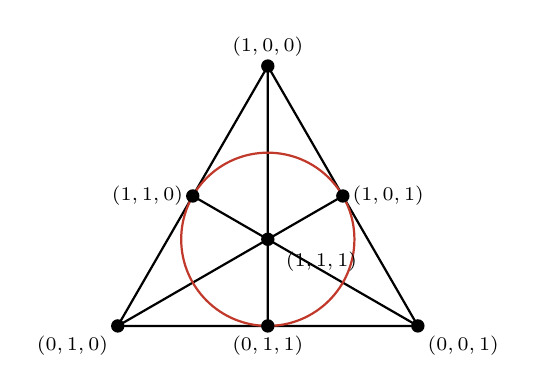
\begin{tikzpicture}[scale=1.1]
  \coordinate (A) at (90:2); \coordinate (B) at (210:2); \coordinate (C) at (330:2);
  \coordinate (G) at (0,0);
  \coordinate (AB) at ($(A)!0.5!(B)$); \coordinate (BC) at ($(B)!0.5!(C)$); \coordinate (CA) at ($(C)!0.5!(A)$);
  \draw[thick] (A)--(B)--(C)--cycle;
  \draw[thick] (A)--(BC) (B)--(CA) (C)--(AB);
  \draw[thick,figred] (G) circle (1);
  \foreach \p in {A,B,C,G,AB,BC,CA} \fill (\p) circle (2.2pt);
  \node[above] at (A) {\scriptsize $(1,0,0)$};
  \node[below left] at (B) {\scriptsize $(0,1,0)$};
  \node[below right] at (C) {\scriptsize $(0,0,1)$};
  \node[left] at (AB) {\scriptsize $(1,1,0)$};
  \node[right] at (CA) {\scriptsize $(1,0,1)$};
  \node[below] at (BC) {\scriptsize $(0,1,1)$};
  \node[below right=1pt and 3pt] at (G) {\scriptsize $(1,1,1)$};
\end{tikzpicture}
\caption{Fano 平面 $PG(2,2)$：7 点 7 线，每线 3 点，每点 3 线（圆也是一条“线”）}
\end{figure}

\subsection{点的齐次坐标}

\begin{defbox}{定义 1.5（齐次坐标）}
在 $\pi_0$ 上取仿射标架 $[O_1;\vv d_1,\vv d_2]$，在 $\pi_0$ 外取一点 $O$，令 $\vv d_3=\overrightarrow{OO_1}$。$\pib$ 上任一点 $M$ 在把 $O$ 中对应直线 $l$ 的任一方向向量在 $[O;\vv d_1,\vv d_2,\vv d_3]$ 下的坐标 $(x_1,x_2,x_3)\T$ 称为 $M$ 的\key{齐次坐标}。
\begin{itemize}
\item $(x_1,x_2,x_3)\T$ 与 $\lambda(x_1,x_2,x_3)\T$（$\lambda\neq0$）表示同一点；$(0,0,0)\T$ 不表示任何点。
\item \key{通常点} $(x,y)\T\ \leftrightarrow\ (x,y,1)\T$，反之 $x=\dfrac{x_1}{x_3},\ y=\dfrac{x_2}{x_3}$（$x_3\neq0$）。
\item \key{无穷远点} $\leftrightarrow$ $x_3=0$：方向 $(u,v)\T$ 的无穷远点是 $(u,v,0)\T$。
\end{itemize}
\end{defbox}

\begin{intbox}{一句话记忆}
“给 $(x,y)$ 后面\key{补一个 1}”就是齐次坐标；“给方向 $(u,v)$ 后面\key{补一个 0}”就是无穷远点。第一章习题 1.2 里“三点共线 $\iff$ 加一行 1 的行列式为 0”的技巧，正是齐次坐标的雏形。
\end{intbox}

\subsection{直线的齐次坐标方程}

设 $A(a_1,a_2,a_3)\T,\ B(b_1,b_2,b_3)\T$ 是不同两点。$M(x_1,x_2,x_3)\T$ 在 $AB$ 上 $\iff$ 把 $O$ 中对应向量共面：
\begin{equation}
\begin{pmatrix}x_1\\x_2\\x_3\end{pmatrix}=\lambda\begin{pmatrix}a_1\\a_2\\a_3\end{pmatrix}+\mu\begin{pmatrix}b_1\\b_2\\b_3\end{pmatrix}\quad(\lambda,\mu\text{ 不全为零})
\iff
\begin{vmatrix}x_1&a_1&b_1\\x_2&a_2&b_2\\x_3&a_3&b_3\end{vmatrix}=0 .
\end{equation}
按第一列展开得 $\eta_1x_1+\eta_2x_2+\eta_3x_3=0$，其中
\[
\eta_1=\begin{vmatrix}a_2&b_2\\a_3&b_3\end{vmatrix},\quad
\eta_2=-\begin{vmatrix}a_1&b_1\\a_3&b_3\end{vmatrix},\quad
\eta_3=\begin{vmatrix}a_1&b_1\\a_2&b_2\end{vmatrix},
\qquad\text{即}\quad (\eta_1,\eta_2,\eta_3)\T=\vv a\times\vv b .
\]

\begin{thmbox}{核心公式（全章反复使用）}
\begin{itemize}
\item 直线 $\iff$ 三元一次\key{齐次}方程 $\eta_1x_1+\eta_2x_2+\eta_3x_3=0$；$(\eta_1,\eta_2,\eta_3)\T$ 称为直线的\key{齐次坐标}（同样差一个倍数）。
\item \key{无穷远直线}：$x_3=0$，坐标 $(0,0,1)\T$。欧氏直线 $ax+by+c=0\ \to\ ax_1+bx_2+cx_3=0$，它的无穷远点是 $(b,-a,0)\T$。
\item 点 $\vv x$ 在线 $\vv\eta$ 上 $\iff \vv\eta\T\vv x=0$（对 $\vv x,\vv\eta$ \key{对称}！）。
\item \key{两点连线} $=\vv a\times\vv b$；\key{两线交点} $=\vv u\times\vv v$。
\item 三点共线 $\iff|\vv a\ \vv b\ \vv c|=0$；三线共点 $\iff|\vv u\ \vv v\ \vv w|=0$。
\end{itemize}
\end{thmbox}

\noindent 叉积公式（按“去掉一行，交叉相乘”记）：$\vv a\times\vv b=(a_2b_3-a_3b_2,\ a_3b_1-a_1b_3,\ a_1b_2-a_2b_1)\T$。

\begin{mtbox}{例：平行线交于无穷远点}
$x-2y+3=0$ 与 $2x-4y+1=0$ 平行。齐次化后交点为
\begin{align*}
(1,-2,3)\T\times(2,-4,1)\T&=\big((-2)\cdot1-3\cdot(-4),\ 3\cdot2-1\cdot1,\ 1\cdot(-4)-(-2)\cdot2\big)\T\\
&=(10,5,0)\T\sim(2,1,0)\T,
\end{align*}
正是两直线的公共方向 $(2,1)$ 的无穷远点。\gd 解方程组 $\begin{cases}x_1-2x_2+3x_3=0\\2x_1-4x_2+x_3=0\end{cases}$ 的基础解系就是两行的叉积（Cramer 法则）。
\end{mtbox}

\paragraph{点方程与线方程。}固定直线 $\vv\eta$，$\vv\eta\T\vv x=0$ 是它上面全体点满足的方程（\key{直线的点方程}）；固定点 $\vv x$，同一个式子是过它的全体直线满足的方程（\key{点的线方程}）。点和线在射影平面上地位对称——这就是下一节对偶原理的来源。

% ---------------- 习题 7.1 ----------------
\xiti{7.1}

\begin{ex}{7.1.1}
设扩大的欧氏平面 $\pib$ 上两点 $A,B$ 的齐次坐标分别是 $(3,-1,2)\T,(2,0,1)\T$，求：(1) 直线 $AB$ 的齐次坐标方程；(2) 直线 $AB$ 上的无穷远点的齐次坐标。
\end{ex}
\jie (1) 用叉积：$\vv a\times\vv b=\big((-1)\cdot1-2\cdot0,\ 2\cdot2-3\cdot1,\ 3\cdot0-(-1)\cdot2\big)\T=(-1,1,2)\T$，所以
\[
AB:\ x_1-x_2-2x_3=0 .
\]
检验：$A$：$3+1-4=0$；$B$：$2-0-2=0$。\quad(2) 令 $x_3=0$ 得 $x_1=x_2$，无穷远点 $(1,1,0)\T$。

\begin{ckbox}{另两种看法（互相验证）}
\textbf{仿射法}：$A=(\tfrac32,-\tfrac12)$，$B=(2,0)$，方向 $\overrightarrow{AB}=(\tfrac12,\tfrac12)\sim(1,1)$，补 0 得 $(1,1,0)\T$。\quad
\textbf{参数法}：$\lambda\vv a+\mu\vv b$ 的第三个分量 $2\lambda+\mu=0$，取 $\lambda=1,\mu=-2$：$(3-4,-1-0,0)\T=(-1,-1,0)\T\sim(1,1,0)\T$。
\end{ckbox}

\begin{ex}{7.1.2}
证明 $\pib$ 上三条直线 $x_1+x_2=0,\ 2x_1-x_2+3x_3=0,\ 5x_1+2x_2+3x_3=0$ 共点，并求该点的齐次坐标。
\end{ex}
\jie 三线共点 $\iff$ 系数行列式为零：
\[
\begin{vmatrix}1&1&0\\2&-1&3\\5&2&3\end{vmatrix}=1\cdot(-3-6)-1\cdot(6-15)+0=-9+9=0 .
\]
公共点 $=(1,1,0)\T\times(2,-1,3)\T=(3,-3,-3)\T\sim(-1,1,1)\T$，验证第三条：$-5+2+3=0$。它是通常点 $(-1,1)$。

\begin{intbox}{直觉}
行列式为零的原因一眼可见：第三行 $=3\times$第一行 $+$ 第二行，$(5,2,3)=3(1,1,0)+(2,-1,3)$。\gd 线性相关的三条“行向量”$\iff$ 三条直线属于同一个线束（见习题 7.2 第 3 题）。
\end{intbox}

\begin{ex}{7.1.3}
在 $\pib$ 上，给出 $\pi_0$ 的欧氏直线的仿射坐标方程，求由它确定的射影直线的齐次坐标方程，并求出射影直线上的无穷远点：(1) $x+2y-1=0$；(2) $x=0$；(3) $y=1$；(4) $3x-2y=0$。
\end{ex}
\jie 代入 $x=x_1/x_3,\ y=x_2/x_3$ 并乘 $x_3$；无穷远点令 $x_3=0$（或直接用“$ax+by+c=0$ 的无穷远点是 $(b,-a,0)\T$”）：
\begin{center}
\renewcommand{\arraystretch}{1.2}
\begin{tabular}{llll}
\toprule
& 欧氏直线 & 齐次方程 & 无穷远点\\\midrule
(1) & $x+2y-1=0$ & $x_1+2x_2-x_3=0$ & $(2,-1,0)\T$\\
(2) & $x=0$ & $x_1=0$ & $(0,1,0)\T$（$y$ 轴方向）\\
(3) & $y=1$ & $x_2-x_3=0$ & $(1,0,0)\T$（$x$ 轴方向）\\
(4) & $3x-2y=0$ & $3x_1-2x_2=0$ & $(2,3,0)\T$\\\bottomrule
\end{tabular}
\end{center}
注意 (4) 过原点、常数项为 0，齐次方程里就没有 $x_3$；(3) 与 $x$ 轴平行，所以无穷远点就是 $x$ 轴的无穷远点 $(1,0,0)\T$。

\begin{ex}{7.1.4}
在 $PG(2,\R)$ 上，设直线 $l_1,l_2,l_3,l_4$ 的方程依次是 $x_1-x_3=0,\ x_2+x_3=0,\ 2x_1+x_2-x_3=0,\ x_1+x_2+2x_3=0$，又设 $l_1$ 与 $l_2$ 的交点为 $A$，$l_3$ 与 $l_4$ 的交点为 $B$，求直线 $AB$ 的方程。
\end{ex}
\jie 全程只用叉积：
\[
A=(1,0,-1)\T\times(0,1,1)\T=(1,-1,1)\T,\qquad
B=(2,1,-1)\T\times(1,1,2)\T=(3,-5,1)\T,
\]
\[
AB=(1,-1,1)\T\times(3,-5,1)\T=(4,2,-2)\T\sim(2,1,-1)\T,\qquad AB:\ 2x_1+x_2-x_3=0 .
\]
\begin{intbox}{直觉}
“线交线得点、点连点得线”用的是\key{同一个运算}——叉积。这正是对偶原理的代数影子：把“点”“线”两个字互换，公式一个字都不用改。
\end{intbox}

\begin{ex}{7.1.5}
取一个球面，用经过球心的一个平面 $\pi$ 截它，取其中一个半球面，把这个半球面上的每个点垂直投影到平面 $\pi$ 上，得到一个圆盘。若投影点在圆盘内部，则把这个投影点看成一个“点”；若投影点在圆盘的边界圆上，则把圆的直径的两个端点看成一个“点”。半球面上的大半圆的投影点组成的半椭圆或直径看成“直线”。证明：这样的圆盘是一个实射影平面。
\end{ex}

\begin{figure}[htbp]
\centering
\begin{tikzpicture}[scale=1.15]
  \fill[defbg] (0,0) circle (1.8); \draw[thick] (0,0) circle (1.8);
  \draw[figred,thick,rotate=-30] (-1.8,0) arc[start angle=180,end angle=360,x radius=1.8,y radius=1.25];
  \draw[figred,thick,rotate=40] (-1.8,0) arc[start angle=180,end angle=0,x radius=1.8,y radius=0.75];
  \draw[figgreen,thick] (-1.8,0)--(1.8,0);
  \fill[figgreen] (-1.8,0) circle (1.6pt) (1.8,0) circle (1.6pt);
  \node[figgreen,left] at (-1.8,0) {\small $Q$}; \node[figgreen,right] at (1.8,0) {\small $Q'$};
  \fill[figpur] (0.45,0.5) circle (1.6pt) node[above right=-2pt,figpur] {\small 内点};
  \node[figred] at (-0.3,1.3) {\small 半椭圆};
  \node[figgreen,below] at (0.2,0) {\small 直径};
  \node[align=center] at (0,-2.35) {\small 边界上的对径点 $Q,Q'$ 视为同一个“点”};
\end{tikzpicture}
\caption{圆盘模型：大圆在上半球的一半投影成半椭圆（平面倾斜）或直径（平面竖直）}
\end{figure}

\zheng 利用球面模型（例 1.3）：球面上“点”= 一对对径点，“线”= 大圆，它是实射影平面。只需在圆盘与球面模型之间建立保持关联的一一对应。

\textbf{点的对应。}一对对径点 $\{A,A'\}$ 中：若不在截面 $\pi$ 上，则恰有一个在所取（开）半球面上，把它投影得圆盘\key{内部}一点；若都在 $\pi$ 上（赤道），则投影就是边界圆上一对\key{直径端点}，按规定合成一个“点”。反之，圆盘内每点是半球面上唯一点的投影，边界上每对直径端点来自赤道上唯一一对对径点。所以“点”$\leftrightarrow$“点”一一对应。

\textbf{线的对应。}大圆由过球心的平面 $\sigma$ 截出。$\sigma\neq\pi$ 时，大圆在半球面上的部分是一个半圆（两端是赤道上一对对径点），其垂直投影是一个以边界直径为长轴的\key{半椭圆}（$\sigma$ 倾斜）或一条\key{直径}（$\sigma\perp\pi$）；$\sigma=\pi$ 时大圆就是赤道，其投影是边界圆（对径点已粘合）。于是“线”$\leftrightarrow$“线”一一对应。

\textbf{关联保持。}点在大圆上 $\iff$ 它的投影在相应半椭圆（直径、边界圆）上，垂直投影保持“在……上”。

综上，圆盘与球面模型之间存在保持关联的点、线一一对应，而球面模型又与把 $O$ 保持关联地一一对应，所以圆盘是实射影平面。\qed

\begin{intbox}{空间直觉}
这个圆盘模型说明射影平面 = “圆盘 + 把边界上对径点粘起来”。沿边界走半圈就回到“同一点”——这正是射影平面\key{不可定向}的来源（它含有一条 Möbius 带）。
\end{intbox}

% ================= §7.2 射影平面上的对偶原理 =================
\Needspace{12\baselineskip}
\section{射影平面上的对偶原理}

上一节看到：$\vv\eta\T\vv x=0$ 对“点坐标 $\vv x$”和“线坐标 $\vv\eta$”是对称的。于是点和线在射影平面上地位对等。

\begin{defbox}{对偶命题}
设 $\varphi(\text{点},\text{线})$ 是关于射影平面上一些点和直线的\key{关联关系}的命题。把其中的“点”都改成“线”、“线”都改成“点”，保持关联关系及其他表述不变，得到的命题 $\varphi(\text{线},\text{点})$ 称为原命题的\key{对偶命题}。
\end{defbox}

\begin{center}
\renewcommand{\arraystretch}{1.3}
\begin{tabularx}{\linewidth}{@{}>{\raggedright\arraybackslash}X|>{\raggedright\arraybackslash}X@{}}
\toprule
\textbf{\sffamily 原命题} & \textbf{\sffamily 对偶命题}\\\midrule
(1) 三点共线 $\iff$ 它们的齐次坐标组成的 3 阶行列式为零 & (1)$'$ 三线共点 $\iff$ 它们的齐次坐标组成的 3 阶行列式为零\\
(2) 若三点 $P_1,P_2,P_3$ 不共线，则三线 $P_1P_2,P_2P_3,P_3P_1$ 不共点 & (2)$'$ 若三线 $p_1,p_2,p_3$ 不共点，则三点 $p_1p_2,p_2p_3,p_3p_1$ 不共线\\
(3) \key{Desargues 定理}：两个三角形对应顶点的连线共点 $\Rightarrow$ 对应边的交点共线 & (3)$'$ \key{Desargues 逆定理}：两个三角形对应边的交点共线 $\Rightarrow$ 对应顶点的连线共点\\
(4) 直线（看成点列）的点方程是三元一次齐次方程 & (4)$'$ 点（看成线束）的线方程是三元一次齐次方程\\\bottomrule
\end{tabularx}
\end{center}

\begin{mtbox}{对偶词典}
\renewcommand{\arraystretch}{1.15}
\begin{tabularx}{\linewidth}{@{}XXX@{}}
点 $\leftrightarrow$ 线 & 共线 $\leftrightarrow$ 共点 & 两点的连线 $\leftrightarrow$ 两线的交点\\
点列（一条线上的点） $\leftrightarrow$ 线束（过一点的线） & 三角形 $\leftrightarrow$ 三角形（自对偶） & 完备四点形 $\leftrightarrow$ 完备四边形\\
点在曲线上 $\leftrightarrow$ 线与曲线相切（\S7.6 配极） & $\vv x=\lambda\vv a+\mu\vv b$ $\leftrightarrow$ $\vv\eta=\lambda\vv u+\mu\vv v$ & 行列式 $=0$ $\leftrightarrow$ 行列式 $=0$
\end{tabularx}
\end{mtbox}

\begin{thmbox}{射影平面上的对偶原理}
射影平面上，如果命题 $\varphi(\text{点},\text{线})$ 是定理，则它的对偶命题 $\varphi(\text{线},\text{点})$ 也是定理。
\end{thmbox}

\textbf{证明思路}：取坐标系，把 $\varphi(\text{点},\text{线})$ 的证明用齐次坐标写出来。在这个证明中把点的坐标都看作线的坐标、线的坐标都看作点的坐标——所有表示关联关系的方程 $\vv\eta\T\vv x=0$ 原封不动，仍然成立，而结论恰好变成了 $\varphi(\text{线},\text{点})$。\qed

\begin{gdbox}{高代联动：对偶空间}
点坐标是\key{列向量} $\vv x\in V=\R^3$，线坐标是\key{行向量} $\vv\eta\T\in V^*$（线性函数），“点在线上”就是 $\vv\eta\T(\vv x)=0$。$V$ 的 1 维子空间（点）$\leftrightarrow$ $V^*$ 的 2 维子空间（零化它的线性函数，即过它的线束）；$V$ 的 2 维子空间（线）$\leftrightarrow$ $V^*$ 的 1 维子空间。对偶原理就是 $V$ 与 $V^*$ 之间这个\key{反序}的一一对应（零化子 $U\mapsto U^\circ$）。
\end{gdbox}

\subsection*{Desargues（德沙格）定理}
\begin{thmbox}{Desargues 定理}
射影平面上，如果两个三角形 $ABC$ 与 $A'B'C'$ 的对应顶点的连线 $AA',BB',CC'$ 共点 $D$，那么它们的对应边的交点
\[
P=AB\cap A'B',\qquad Q=AC\cap A'C',\qquad R=BC\cap B'C'
\]
共线。由对偶原理，它的逆定理（对偶命题）也成立。
\end{thmbox}

\begin{figure}[htbp]
\centering
\begin{tikzpicture}[scale=0.92]
  \coordinate (D) at (0,0);
  \coordinate (A) at (2.33,1.18); \coordinate (B) at (2.98,-0.33); \coordinate (C) at (2.06,-1.24);
  \coordinate (A') at (3.4,1.71); \coordinate (B') at (5.45,-0.6); \coordinate (C') at (4.93,-2.97);
  \coordinate (P) at (intersection of A--B and A'--B');
  \coordinate (Q) at (intersection of A--C and A'--C');
  \coordinate (R) at (intersection of B--C and B'--C');
  \draw[figgray,dashed] (D)--(A') (D)--(B') (D)--(C');
  \fill[figblue!12] (A)--(B)--(C)--cycle; \fill[figred!12] (A')--(B')--(C')--cycle;
  \draw[figblue,thick] (A)--(B)--(C)--cycle; \draw[figred,thick] (A')--(B')--(C')--cycle;
  \draw[figblue!70,dotted,thick] (B)--(P) (C)--(Q) (C)--(R);
  \draw[figred!70,dotted,thick] (B')--(P) (C')--(Q) (C')--(R);
  \draw[figgreen,very thick] ($(P)!-0.12!(R)$)--($(P)!1.12!(R)$);
  \foreach \p/\pos in {D/left,A/above left,B/below left,C/below left,A'/above,B'/right,C'/right}{\fill (\p) circle (1.6pt) node[\pos] {$\p$};}
  \foreach \p in {P,Q,R}{\fill[figgreen] (\p) circle (2pt) node[above right,figgreen] {$\p$};}
  \node[figgreen,rotate=-12,above] at ($(Q)!0.5!(R)+(0,0.12)$) {\small Desargues 轴};
\end{tikzpicture}
\caption{Desargues 定理：透视中心 $D$ $\Rightarrow$ 透视轴 $PQR$}
\end{figure}

\zheng 若某对对应顶点重合（如 $A=A'$），则 $P=Q=A$，结论显然。设对应顶点都不重合，各点齐次坐标记为小写黑体。$D$ 在 $AA',BB',CC'$ 上，故存在不全为零的数使
\begin{equation}
\vv d=\lambda\vv a+\lambda'\vv a'=\mu\vv b+\mu'\vv b'=\nu\vv c+\nu'\vv c'.
\end{equation}
移项（“把带撇的放一边”）：
\[
\vv p:=\lambda\vv a-\mu\vv b=-\lambda'\vv a'+\mu'\vv b',\quad
\vv q:=-\lambda\vv a+\nu\vv c=\lambda'\vv a'-\nu'\vv c',\quad
\vv r:=\mu\vv b-\nu\vv c=-\mu'\vv b'+\nu'\vv c'.
\]
$\vv p$ 既是 $\vv a,\vv b$ 的组合又是 $\vv a',\vv b'$ 的组合，所以它表示 $AB\cap A'B'=P$；同理 $\vv q$ 表示 $Q$，$\vv r$ 表示 $R$。而
\[
\vv p+\vv q+\vv r=\vv0,
\]
三个向量线性相关，故 $P,Q,R$ 共线。\qed

\begin{intbox}{空间直觉：Desargues 是“空间里显然的事”的投影}
如果两个三角形在空间中\key{两个不同平面} $\sigma,\sigma'$ 上，且 $AA',BB',CC'$ 交于 $D$：$AB$ 与 $A'B'$ 都在平面 $DAB$ 内，必相交，交点 $P$ 既在 $\sigma$ 上又在 $\sigma'$ 上——即在交线 $\sigma\cap\sigma'$ 上。$Q,R$ 同理，所以 $P,Q,R$ 都在 $\sigma\cap\sigma'$ 这条直线上。把整个图形投影到一个平面上，就是平面 Desargues 定理。上面的代数证明 $\vv p+\vv q+\vv r=\vv0$ 正是这个空间图形的“影子”。
\end{intbox}

% ---------------- 习题 7.2 ----------------
\xiti{7.2}

\begin{ex}{7.2.1}
证明：射影平面上，若 $P_1,P_2,P_3$ 三点不共线，则 $P_1P_2,P_2P_3,P_3P_1$ 三线不共点。
\end{ex}
\zheng\textbf{方法一（关联性质）}：若三线共点 $Q$。$P_1P_2\neq P_2P_3$（否则三点共线），两条不同直线只有一个交点，而 $P_2$ 是它们的公共点，故 $Q=P_2$；同理由 $P_2P_3,P_3P_1$ 得 $Q=P_3$。于是 $P_2=P_3$，矛盾。

\textbf{方法二（坐标，提示所说的“两个矩阵的关系”）}：设 $\Pi=(\vv p_1,\vv p_2,\vv p_3)$，$|\Pi|\neq0$。三条线的坐标
\[
\vv u_1=\vv p_2\times\vv p_3\ (P_2P_3),\quad \vv u_2=\vv p_3\times\vv p_1\ (P_3P_1),\quad \vv u_3=\vv p_1\times\vv p_2\ (P_1P_2).
\]
由混合积，$\vv u_i\T\vv p_j=\delta_{ij}|\Pi|$，即 $U\T\Pi=|\Pi|\,I$（$U=(\vv u_1,\vv u_2,\vv u_3)$）。取行列式：$|U|\cdot|\Pi|=|\Pi|^3$，所以
\[
|U|=|\Pi|^2\neq0,
\]
三线不共点。\qed

\begin{gdbox}{高代}
$U\T=|\Pi|\,\Pi^{-1}=\Pi^*$（伴随矩阵），$|\Pi^*|=|\Pi|^{n-1}=|\Pi|^2$。“三角形三边的坐标”就是“三顶点坐标矩阵的伴随”——这就是对偶的矩阵形式。
\end{gdbox}

\begin{ex}{7.2.2}
设命题 $\varphi(\text{点},\text{线})$ 为：在射影平面上，$A,B,C$ 和 $A',B',C'$ 分别是直线 $l_1$ 和 $l_2$ 上的三个点，并且均与 $l_1$ 和 $l_2$ 的交点 $D$ 不重合。设 $AB'$ 与 $A'B$ 交于点 $P$，$BC'$ 与 $B'C$ 交于点 $Q$，$CA'$ 与 $C'A$ 交于点 $R$，则 $P,Q,R$ 三点共线。试写出这个命题的对偶命题 $\varphi(\text{线},\text{点})$。
\end{ex}
\jie 原命题就是 \key{Pappus 定理}（习题 7.4 第 5 题证明）。逐词对偶：“直线 $l_1,l_2$ 上的点”$\to$“过点 $P,P'$ 的线”；“与交点 $D$ 不重合”$\to$“与连线 $PP'$ 不重合”；“$AB'$ 与 $A'B$ 的交点”$\to$“$l_1\cap l_2'$ 与 $l_1'\cap l_2$ 的连线”；“共线”$\to$“共点”。

\begin{thmbox}{对偶命题（Pappus 定理的对偶）}
在射影平面上，$l_1,l_2,l_3$ 和 $l_1',l_2',l_3'$ 分别是过点 $P$ 和 $P'$ 的三条直线，并且均与直线 $PP'$ 不重合。设
\[
A=l_1\cap l_2',\ A'=l_1'\cap l_2,\quad B=l_2\cap l_3',\ B'=l_2'\cap l_3,\quad C=l_3\cap l_1',\ C'=l_3'\cap l_1,
\]
则 $AA',\ BB',\ CC'$ 三线共点。
\end{thmbox}

\begin{figure}[htbp]
\centering
\begin{tikzpicture}[scale=0.95]
  \coordinate (P) at (0,0); \coordinate (P') at (8,-0.76);
  \coordinate (A) at (4.63,2.87); \coordinate (A') at (2.37,2.07);
  \coordinate (B) at (5.36,4.68); \coordinate (B') at (2.29,5.39);
  \coordinate (C) at (1.14,2.69); \coordinate (C') at (5.86,3.64);
  \coordinate (O) at (intersection of A--A' and B--B');
  \foreach \t/\n in {31.8/1,41.1/2,66.9/3}{\draw[figblue] (P)--++(\t:{\n==1?7.2:(\n==2?7.6:6.3)}) node[right,figblue] {\small $l_\n$};}
  \foreach \t/\n in {153.3/1,132.9/2,115.9/3}{\draw[figred] (P')--++(\t:{\n==1?8.3:(\n==2?8.1:7.0)}) node[left,figred] {\small $l'_\n$};}
  \draw[figgray,dashed] (P)--(P');
  \draw[figgreen,thick] ($(A')!-0.25!(O)$)--($(A')!1.08!(O)$);
  \draw[figgreen,thick] ($(B')!-0.08!(O)$)--($(B')!1.08!(O)$);
  \draw[figgreen,thick] ($(C)!-0.08!(O)$)--($(C)!1.08!(O)$);
  \foreach \p/\pos in {P/below left,P'/below right,A/below,A'/below left,B/above,B'/above left,C/left,C'/below right}{\fill (\p) circle (1.6pt) node[\pos] {\small $\p$};}
  \fill[keyred] (O) circle (2.2pt) node[above=3pt,keyred] {\small 共点};
\end{tikzpicture}
\caption{Pappus 定理的对偶：两个线束 $P,P'$ 交出的六点，$AA',BB',CC'$ 共点}
\end{figure}

\begin{ex}{7.2.3}
设射影平面上直线 $l_i$ 的齐次坐标为 $(\eta_{i1},\eta_{i2},\eta_{i3})\T$ $(i=1,2,3)$，并且 $l_1\neq l_2$。证明：$l_1,l_2,l_3$ 共点的充分必要条件是，存在不全为零的实数 $\lambda$ 和 $\mu$，使得 $\eta_{3j}=\lambda\eta_{1j}+\mu\eta_{2j}$，$j=1,2,3$。
\end{ex}
\zheng 记 $\vv\eta_i=(\eta_{i1},\eta_{i2},\eta_{i3})\T$。

\textbf{充分性}：设 $\vv\eta_3=\lambda\vv\eta_1+\mu\vv\eta_2$。$l_1,l_2$ 的交点 $X$ 满足 $\vv\eta_1\T\vv x=\vv\eta_2\T\vv x=0$，于是 $\vv\eta_3\T\vv x=\lambda\cdot0+\mu\cdot0=0$，$X$ 也在 $l_3$ 上。

\textbf{必要性}：设三线共点 $X(\vv x)$。则 $\vv\eta_1,\vv\eta_2,\vv\eta_3$ 都属于
\[
W=\{\vv u\in\R^3:\ \vv u\T\vv x=0\},
\]
它是一个齐次线性方程的解空间，$\dim W=3-1=2$。$l_1\neq l_2$ 说明 $\vv\eta_1,\vv\eta_2$ 线性无关，因而是 $W$ 的一个基，所以 $\vv\eta_3=\lambda\vv\eta_1+\mu\vv\eta_2$；又 $\vv\eta_3\neq\vv0$，故 $\lambda,\mu$ 不全为零。\qed

\begin{intbox}{直觉}
这正是“点 $X$ 在直线 $AB$ 上 $\iff \vv x=\lambda\vv a+\mu\vv b$”（直线的参数方程）的对偶：\key{过一点的线束} $=\{\lambda\vv\eta_1+\mu\vv\eta_2\}$。在仿射图形里，$\lambda(A_1x+B_1y+C_1)+\mu(A_2x+B_2y+C_2)=0$ 就是第二章熟悉的“过两直线交点的直线系”（两直线平行时是平行线系——交于无穷远点）。
\end{intbox}

\begin{ex}{7.2.4$^*$}
设 $M$ 是欧氏平面 $\pi_0$ 上的一点，$l_1$ 和 $l_2$ 是 $\pi_0$ 上的两条直线，它们相交于一个不可到达的点 $N$（非常远或被物体阻隔）。试用直尺作经过点 $M$ 和 $N$ 的直线。
\end{ex}
\fenxi 想让“$l_1,l_2$ 和所求直线 $MM'$ 共点于 $N$”——这是“对应顶点连线共点”，用 \key{Desargues 逆定理}：只要造一个三角形 $A'B'M'$ 与 $\triangle ABM$ 的\key{对应边交点共线}，其中 $A,A'\in l_1$，$B,B'\in l_2$，那么 $AA'=l_1$、$BB'=l_2$、$MM'$ 三线共点。

\jie\textbf{作法}：
\begin{enumerate}
\item 在 $l_1,l_2$ 外取一点 $P$，过 $P$ 作两条直线，分别交 $l_1,l_2$ 于 $A,B$ 和 $A',B'$（于是 $AB\cap A'B'=P$）；
\item 过 $P$ 再作一条直线 $s$（作为“透视轴”），设 $AM$ 交 $s$ 于 $X$，$BM$ 交 $s$ 于 $Y$；
\item 连 $A'X$、$B'Y$，交于 $M'$；
\item 直线 $MM'$ 即为所求。
\end{enumerate}
\textbf{理由}：$\triangle ABM$ 与 $\triangle A'B'M'$ 的对应边交点 $AB\cap A'B'=P$，$AM\cap A'M'=X$，$BM\cap B'M'=Y$ 都在 $s$ 上（共线）。由 Desargues 逆定理，对应顶点连线 $AA'=l_1$、$BB'=l_2$、$MM'$ 共点，即 $MM'$ 过 $N$。\qed

\begin{figure}[htbp]
\centering
\begin{tikzpicture}[scale=1.0]
  \begin{scope}
  \clip (-0.4,-2.1) rectangle (7.6,4.4);
  \coordinate (N) at (14.02,2.89);
  \coordinate (M) at (1.9,2.18); \coordinate (P) at (3.23,-0.67);
  \coordinate (A) at (3.03,0.63); \coordinate (B) at (2.59,3.47);
  \coordinate (A') at (4.49,0.93); \coordinate (B') at (6.35,3.28);
  \coordinate (X) at (4.72,-1.69); \coordinate (Y) at (1.15,0.76);
  \coordinate (M') at (intersection of A'--X and B'--Y);
  \draw[thick] (0,0)--(N); \draw[thick] (0,3.6)--(N);
  \draw[figgray] ($(P)!-0.15!(B)$)--($(P)!1.12!(B)$);
  \draw[figgray] ($(P)!-0.15!(B')$)--($(P)!1.1!(B')$);
  \draw[figor,thick] ($(Y)!-0.25!(X)$)--($(Y)!1.15!(X)$);
  \draw[figblue] (A)--(M)--(B) (A)--(X) (B)--(Y);
  \draw[figred] (A')--(M')--(B') (A')--(X) (B')--(Y);
  \draw[figgreen,very thick,dashed] (M)--($(M)!3.2!(M')$);
  \foreach \p/\pos in {M/above left,P/below left,A/below right,B/above,A'/below right,B'/above,X/below,Y/left,M'/above}{\fill (\p) circle (1.6pt) node[\pos] {\small $\p$};}
  \end{scope}
  \node at (7.85,1.7) {\small $l_1$}; \node at (7.85,3.85) {\small $l_2$};
  \node[figor] at (0.4,1.55) {\small $s$};
  \draw[->,keyred,thick] (7.6,2.6)--(8.5,2.75) node[right,keyred,align=left] {\small 交点 $N$\\\small 在纸外};
\end{tikzpicture}
\caption{用 Desargues 逆定理作过不可到达点 $N$ 的直线（绿色虚线）}
\end{figure}

% ================= §7.3 交比 =================
\Needspace{12\baselineskip}
\section{交比}

中心投影不保持分比（中点的像一般不是中点），但有一个由\key{四个}共线点算出的数保持不变——交比。它是射影几何里唯一的“度量”。

\subsection{交比的定义和性质}

\begin{defbox}{定比与交比（定义 3.1）}
\textbf{定比}：$A,B$ 为通常点，$C\neq B$ 共线。若 $\overrightarrow{AC}=\lambda\overrightarrow{CB}$，记 $(A,B,C)=\lambda=\dfrac{AC}{CB}$（代数长之比）；$C$ 为无穷远点时规定 $(A,B,C)=-1$。\\[2pt]
\textbf{交比}：$A,B,C,D$ 共线，$A,B$ 为通常点，$A\neq B$，$C\neq B$，$D\neq A,B$，
\begin{equation}
(A,B;C,D):=\frac{(A,B,C)}{(A,B,D)}=\frac{AC}{CB}\Big/\frac{AD}{DB}=\frac{AC}{CB}\cdot\frac{DB}{AD}.
\end{equation}
$A,B,C$ 各不相同时规定 $D=B$ 时 $(A,B;C,D)=0$。交比也叫\key{二重比}——“两个分比之比”。
\end{defbox}

\begin{thmbox}{二级结论：数轴坐标公式（最常用）}
若 $A,B,C,D$ 在一条数轴上的坐标为 $a,b,c,d$，则
\[
(A,B;C,D)=\frac{(c-a)(d-b)}{(c-b)(d-a)},\qquad (A,B;C,\infty)=\frac{c-a}{c-b}=\frac{AC}{BC}.
\]
\ji “$C$ 减 $A$、$D$ 减 $B$”在分子，“$C$ 减 $B$、$D$ 减 $A$”在分母——\key{分子交叉配对，分母同侧配对}。
\end{thmbox}

\begin{figure}[htbp]
\centering
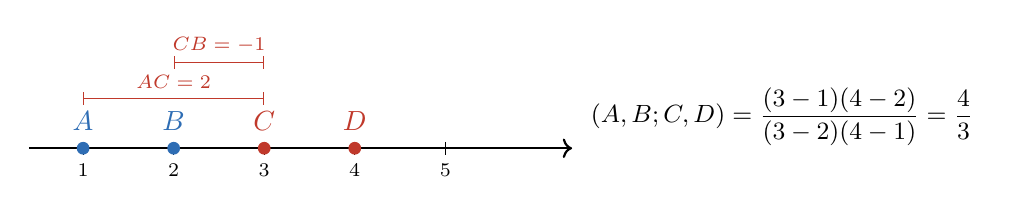
\begin{tikzpicture}[scale=1.15]
  \draw[->,thick] (-0.6,0)--(5.4,0);
  \foreach \x/\n in {0/1,1/2,2/3,3/4,4/5}{\draw (\x,0.07)--(\x,-0.07) node[below] {\scriptsize $\n$};}
  \foreach \x/\p/\c in {0/A/figblue,1/B/figblue,2/C/figred,3/D/figred}{\fill[\c] (\x,0) circle (2pt) node[above=3pt,\c] {$\p$};}
  \draw[figred,|-|] (0,0.55)--node[above] {\scriptsize $AC=2$} (2,0.55);
  \draw[figred,|-|] (2,0.95)--node[above] {\scriptsize $CB=-1$} (1,0.95);
  \node[align=left,right] at (5.5,0.35) {\small $(A,B;C,D)=\dfrac{(3-1)(4-2)}{(3-2)(4-1)}=\dfrac43$};
\end{tikzpicture}
\caption{例：坐标 $1,2,3,4$ 的四点，交比为 $\frac43$（注意 $C$ 在线段 $AB$ 外，所以 $(A,B,C)=-2<0$）}
\end{figure}

\paragraph{共点四线的交比。}设 $l_1,l_2,l_3,l_4$ 过点 $O$，$l_1\neq l_2$。任取一条不过 $O$ 的截线 $l$，交 $l_i$ 于 $A_i$，规定
\begin{equation}
(l_1,l_2;l_3,l_4):=(A_1,A_2;A_3,A_4).
\end{equation}
这个定义与截线的选取无关：若线坐标满足 $\vv\eta_3=\lambda_1\vv\eta_1+\mu_1\vv\eta_2$，$\vv\eta_4=\lambda_2\vv\eta_1+\mu_2\vv\eta_2$（习题 7.2 第 3 题），则
\begin{equation}
(l_1,l_2;l_3,l_4)=\frac{\lambda_2}{\mu_2}\Big/\frac{\lambda_1}{\mu_1},
\end{equation}
右端只与四条直线有关。

\begin{figure}[htbp]
\centering
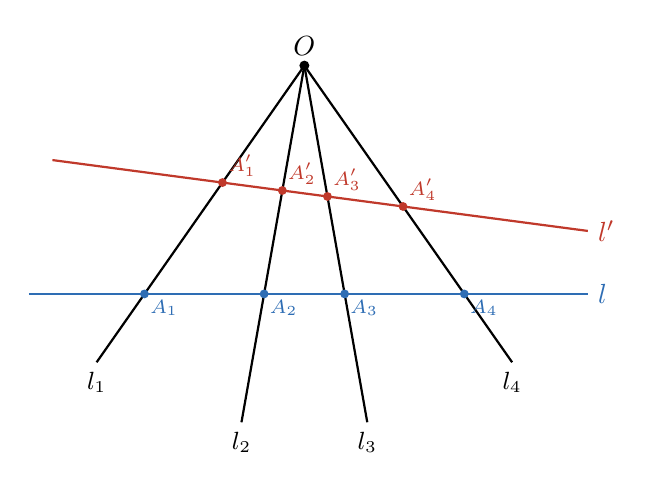
\begin{tikzpicture}[scale=1.0]
  \coordinate (O) at (0,3.2);
  \coordinate (T1a) at (-3.5,0.3); \coordinate (T1b) at (3.6,0.3);
  \coordinate (T2a) at (-3.2,2.0); \coordinate (T2b) at (3.6,1.1);
  \draw[figblue,thick] (T1a)--(T1b) node[right] {$l$};
  \draw[figred,thick] (T2a)--(T2b) node[right] {$l'$};
  \foreach \a/\i in {-125/1,-100/2,-80/3,-55/4}{
    \coordinate (E) at ($(O)+(\a:4.6)$);
    \draw[thick] (O)--(E) node[below] {\small $l_\i$};
    \coordinate (X) at (intersection of O--E and T1a--T1b);
    \coordinate (Y) at (intersection of O--E and T2a--T2b);
    \fill[figblue] (X) circle (1.6pt) node[below right=-2pt,figblue] {\scriptsize $A_\i$};
    \fill[figred] (Y) circle (1.6pt) node[above right=-2pt,figred] {\scriptsize $A'_\i$};}
  \fill (O) circle (1.8pt) node[above] {$O$};
\end{tikzpicture}
\caption{同一线束被两条截线截得的四点交比相等：$(A_1,A_2;A_3,A_4)=(A'_1,A'_2;A'_3,A'_4)$}
\end{figure}

\begin{thmbox}{交比在中心投影下不变}
以 $O$ 为中心的中心投影把 $l$ 上的 $A_i$ 投成 $l'$ 上的 $A'_i$，而 $A_i,A_i'$ 都在 $l_i$ 上，所以
\[
(A_1,A_2;A_3,A_4)=(l_1,l_2;l_3,l_4)=(A'_1,A'_2;A'_3,A'_4).
\]
于是交比的定义可以推广到含无穷远点的情形：总可以先投影成四个通常点再算。
\end{thmbox}

\begin{thmbox}{定理 3.1（用齐次坐标算交比）}
$A,B,C$ 各不相同，$D\neq A$。若 $\vv c=\lambda_1\vv a+\mu_1\vv b$，$\vv d=\lambda_2\vv a+\mu_2\vv b$，则
\begin{equation}
(A,B;C,D)=\frac{\lambda_2}{\mu_2}\Big/\frac{\lambda_1}{\mu_1}.
\end{equation}
\ji “$D$ 的系数比 $\div$ $C$ 的系数比”。注意结果与 $\vv a,\vv b,\vv c,\vv d$ 各自乘什么倍数无关（倍数在比中约掉）。
\end{thmbox}

\noindent\textbf{验证与数轴公式一致}：$\vv a=(a,1)\T,\vv b=(b,1)\T$，$\vv c=(c,1)\T=\lambda_1\vv a+\mu_1\vv b$ 解得 $\frac{\lambda_1}{\mu_1}=\frac{b-c}{c-a}$，同理 $\frac{\lambda_2}{\mu_2}=\frac{b-d}{d-a}$，相除即得 $\frac{(c-a)(d-b)}{(c-b)(d-a)}$。

\begin{thmbox}{定理 3.2（取同一直线上任意两点作“基”）}
在此直线上取两点 $P,Q$，设 $\vv a=\lambda_1\vv p+\mu_1\vv q,\ \vv b=\lambda_2\vv p+\mu_2\vv q,\ \vv c=\lambda_3\vv p+\mu_3\vv q,\ \vv d=\lambda_4\vv p+\mu_4\vv q$，记 $[ij]=\begin{vmatrix}\lambda_i&\lambda_j\\\mu_i&\mu_j\end{vmatrix}$，则
\begin{equation}
(A,B;C,D)=\frac{[13]\,[24]}{[14]\,[23]} .
\end{equation}
\end{thmbox}

\begin{gdbox}{高代联动}
射影直线 = $\R^2$ 的 1 维子空间全体；点 $\leftrightarrow (\lambda_i:\mu_i)$。$[ij]$ 是 2 阶行列式，换基（可逆线性替换 $H$）时每个 $[ij]$ 都乘同一个 $|H|$，每个向量的倍数也在分子分母中各出现一次——所以交比是\key{射影不变量}。公式与数轴公式同形：$[ij]$ 扮演“$x_j-x_i$”。
\end{gdbox}

\begin{thmbox}{交比的性质（24 种排列只有 6 个值）}
(1) $(C,D;A,B)=(A,B;C,D)=(B,A;D,C)$\quad（同时交换两对，值不变）\\
(2) $(B,A;C,D)=\dfrac{1}{(A,B;C,D)}=(A,B;D,C)$\quad（交换一对中的两点，取倒数）\\
(3) $(A,C;B,D)=1-(A,B;C,D)$\quad（交换中间两点，取“1 减”）
\end{thmbox}

\begin{thmbox}{共点四线交比的正弦公式}
$O$ 为通常点，$\langle l_i,l_j\rangle$ 表示 $l_i$ 绕 $O$ 逆时针转到 $l_j$ 的角，则
\begin{equation}
(l_1,l_2;l_3,l_4)=\frac{\sin\langle l_1,l_3\rangle}{\sin\langle l_3,l_2\rangle}\Big/\frac{\sin\langle l_1,l_4\rangle}{\sin\langle l_4,l_2\rangle}.
\end{equation}
（证明见习题 7.3 第 8 题。）与点的公式 $\frac{AC}{CB}\big/\frac{AD}{DB}$ 完全同形：\key{“线段”换成“角的正弦”}。
\end{thmbox}

\subsection{调和点列与调和线束}

\begin{defbox}{定义 3.2（调和）}
共线四点满足 $(A,B;C,D)=-1$，称为\key{调和点列}，$D$ 称为 $A,B,C$ 的\key{第四调和点}，$C,D$ 关于 $A,B$ \key{调和共轭}。由性质 (1)(2)，此时 $A,B$ 也关于 $C,D$ 调和共轭——两个点偶\key{彼此调和分割}。共点四线 $(l_1,l_2;l_3,l_4)=-1$ 称为\key{调和线束}。
\end{defbox}

\begin{thmbox}{二级结论：调和点列的几种等价形式}
\begin{itemize}
\item 数轴坐标：$(A,B;C,D)=-1\iff 2(ab+cd)=(a+b)(c+d)$。
\item $A$ 取为原点：$\dfrac{2}{AB}=\dfrac{1}{AC}+\dfrac{1}{AD}$（$AB$ 是 $AC,AD$ 的\key{调和平均}）。
\item $O$ 为 $AB$ 中点：$OC\cdot OD=OA^2$（Newton 形式）。
\item \key{中点与无穷远点调和共轭}：$C$ 为 $AB$ 中点 $\iff$ $D=\infty$。（因为 $(A,B;C,\infty)=\frac{AC}{BC}=-1$。）
\item \key{两直线的两条角平分线}关于这两直线调和共轭（由正弦公式，见下图）。
\end{itemize}
\end{thmbox}

\begin{mtbox}{例：求调和共轭点}
$A=0,\ B=3,\ C=1$，求 $D$ 使 $(A,B;C,D)=-1$。\quad 由 $\frac{2}{3}=\frac11+\frac1d$ 得 $d=-3$。\\
检验 Newton 形式：中点 $O=1.5$，$OC\cdot OD=(-0.5)(-4.5)=2.25=1.5^2$。 \checkmark
\end{mtbox}

\begin{figure}[htbp]
\centering
\begin{minipage}{0.42\linewidth}\centering
\begin{tikzpicture}[scale=1.0]
  \coordinate (O) at (0,0);
  \draw[thick] (200:2.6)--(20:2.6) node[right] {$l_1$};
  \draw[thick] (-40:2.6)--(140:2.6) node[left] {$l_2$};
  \draw[figred,thick] (-100:2.2)--(80:2.2) node[above] {$l_3$};
  \draw[figblue,thick] (170:2.6)--(-10:2.6) node[right] {$l_4$};
  \draw[figred] (20:0.7) arc (20:80:0.7); \draw[figred] (80:0.8) arc (80:140:0.8);
  \draw[figblue] (140:1.1) arc (140:170:1.1); \draw[figblue] (170:1.2) arc (170:200:1.2);
  \fill (O) circle (1.5pt);
  \node[align=center] at (0,-2.7) {\small $l_3\perp l_4$，都平分 $l_1,l_2$ 的夹角};
\end{tikzpicture}
\end{minipage}\hfill
\begin{minipage}{0.55\linewidth}\centering
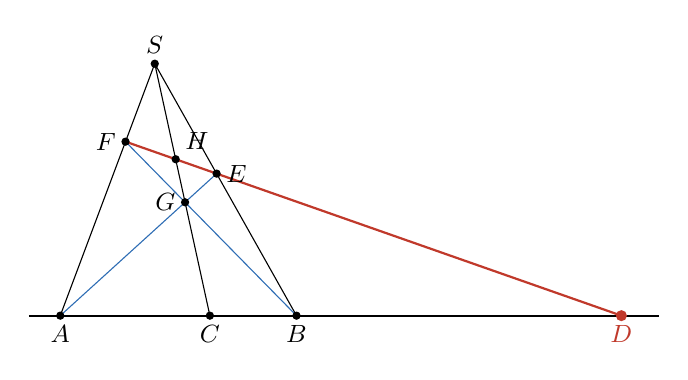
\begin{tikzpicture}[scale=1.0]
  \coordinate (A) at (0,0); \coordinate (B) at (3,0); \coordinate (C) at (1.9,0);
  \coordinate (S) at (1.2,3.2); \coordinate (G) at ($(S)!0.55!(C)$);
  \coordinate (E) at (intersection of A--G and S--B);
  \coordinate (F) at (intersection of B--G and S--A);
  \coordinate (D) at (intersection of F--E and A--B);
  \coordinate (H) at (intersection of F--E and S--C);
  \draw[thick] (-0.4,0)--(7.6,0);
  \draw (A)--(S)--(B) (S)--(C);
  \draw[figblue] (A)--(E) (B)--(F);
  \draw[figred,thick] (F)--(D);
  \foreach \p/\pos in {A/below,B/below,C/below,S/above,G/left,E/right,F/left,H/above right}{\fill (\p) circle (1.5pt) node[\pos] {\small $\p$};}
  \fill[keyred] (D) circle (2pt) node[below,keyred] {\small $D$};
\end{tikzpicture}
\end{minipage}
\caption{左：角平分线构成调和线束；右：只用直尺作第四调和点 $D$}
\end{figure}

\begin{mtbox}{只用直尺作第四调和点（图右）}
在 $AB$ 外任取一点 $S$，连 $SA,SB,SC$；在 $SC$ 上取一点 $G\ (\neq C,S)$，$AG$ 交 $SB$ 于 $E$，$BG$ 交 $SA$ 于 $F$；则 $FE$ 与 $AB$ 的交点 $D$ 就是 $A,B,C$ 的第四调和点。\\[2pt]
\textbf{证明}：设 $FE$ 交 $SC$ 于 $H$。先以 $S$ 为中心、再以 $G$ 为中心作投影：
\[
(A,B;C,D)\overset{S}{=}(F,E;H,D)\overset{G}{=}(B,A;C,D)=\frac{1}{(A,B;C,D)},
\]
所以 $(A,B;C,D)^2=1$。若 $(A,B;C,D)=1$，则 $(A,C;B,D)=0$，推出 $A=B$，矛盾。故 $(A,B;C,D)=-1$。\qed
\end{mtbox}

\begin{intbox}{直觉：为什么是“$-1$”}
令 $S$ 跑到无穷远（$SA,SB,SC$ 变成三条平行线），图就成了一个梯形及其对角线：这时 $C$ 若是 $AB$ 中点，$EF\parallel AB$，$D=\infty$——恰好就是“中点 $\leftrightarrow$ 无穷远点”这对调和共轭。一般情形是它的射影像。
\end{intbox}

% ---------------- 习题 7.3 ----------------
\xiti{7.3}

\begin{ex}{7.3.1}
在射影平面 $\pib$ 上，设共线三点 $A,B,C$ 的齐次坐标分别为 $(1,2,5)\T,(1,0,3)\T,(-1,2,-1)\T$，在直线 $AB$ 上求一点 $D$，使得交比 $(A,B;C,D)=5$。
\end{ex}
\jie 先把 $\vv c$ 写成 $\vv a,\vv b$ 的组合：$\lambda_1\vv a+\mu_1\vv b=\vv c$，比较第二分量 $2\lambda_1=2$ 得 $\lambda_1=1$，再由第一分量 $1+\mu_1=-1$ 得 $\mu_1=-2$（第三分量 $5-6=-1$ \checkmark）。所以 $\frac{\lambda_1}{\mu_1}=-\frac12$。

由定理 3.1，需 $\frac{\lambda_2}{\mu_2}=5\cdot\left(-\frac12\right)=-\frac52$，取 $\lambda_2=-5,\mu_2=2$：
\[
\vv d=-5(1,2,5)\T+2(1,0,3)\T=(-3,-10,-19)\T\sim(3,10,19)\T .
\]

\begin{ex}{7.3.2}
在 $\pib$ 上，设三点 $A,B,C$ 的齐次坐标分别为 $(1,4,1)\T,(0,1,1)\T,(2,3,-3)\T$，证明 $A,B,C$ 三点共线，并且求此直线上的一点 $D$，使得 $(A,B;C,D)=-4$。
\end{ex}
\jie $\begin{vmatrix}1&0&2\\4&1&3\\1&1&-3\end{vmatrix}=1\cdot(-3-3)-0+2\cdot(4-1)=0$，共线。$\vv c=\lambda_1\vv a+\mu_1\vv b$：第一分量 $\lambda_1=2$，第二分量 $8+\mu_1=3$，$\mu_1=-5$（第三分量 $2-5=-3$ \checkmark），$\frac{\lambda_1}{\mu_1}=-\frac25$。需 $\frac{\lambda_2}{\mu_2}=-4\cdot\left(-\frac25\right)=\frac85$：
\[
\vv d=8(1,4,1)\T+5(0,1,1)\T=(8,37,13)\T .
\]

\begin{ex}{7.3.3}
在 $\pib$ 上，给了共线的四个通常点的仿射坐标 $A(2,-4)\T,B(-4,5)\T,C(4,-7)\T,D(0,-1)\T$，求它们的交比 $(A,B;C,D)$。
\end{ex}
\jie 平行于 $y$ 轴投影到 $x$ 轴不改变分比，所以直接用横坐标 $a=2,b=-4,c=4,d=0$：
\[
(A,B;C,D)=\frac{(c-a)(d-b)}{(c-b)(d-a)}=\frac{2\cdot4}{8\cdot(-2)}=-\frac12 .
\]
\textbf{按定义验算}：$\overrightarrow{AC}=(2,-3)$，$\overrightarrow{CB}=(-8,12)$，$\frac{AC}{CB}=-\frac14$；$\overrightarrow{AD}=(-2,3)$，$\overrightarrow{DB}=(-4,6)$，$\frac{AD}{DB}=\frac12$；交比 $=-\frac14\big/\frac12=-\frac12$。

\begin{ex}{7.3.4}
在 $\pib$ 上，设共点于 $O$ 的三条直线 $l_1,l_2,l_3$ 的齐次坐标分别为 $(-1,0,2)\T,(3,1,-2)\T,(1,1,2)\T$，求经过 $O$ 的一条直线 $l_4$，使得交比 $(l_1,l_2;l_3,l_4)=-3$。
\end{ex}
\jie 线束里一切照搬点列的公式。$\vv\eta_3=\lambda_1\vv\eta_1+\mu_1\vv\eta_2$：第二分量 $\mu_1=1$，第一分量 $-\lambda_1+3=1$，$\lambda_1=2$（第三分量 $4-2=2$ \checkmark），$\frac{\lambda_1}{\mu_1}=2$。需 $\frac{\lambda_2}{\mu_2}=-3\cdot2=-6$：
\[
\vv\eta_4=-6(-1,0,2)\T+(3,1,-2)\T=(9,1,-14)\T,\qquad l_4:\ 9x_1+x_2-14x_3=0 .
\]

\begin{ex}{7.3.5}
在 $\pib$ 上，设五个点 $P,A,B,C,D$ 的齐次坐标分别为 $(3,-3,1)\T,(1,0,0)\T,(0,1,0)\T,(0,0,1)\T,(1,-1,1)\T$，求直线 $PA,PB,PC,PD$ 的交比。
\end{ex}
\jie 用叉积求四条直线：
\[
PA=(0,1,3)\T,\quad PB=(-1,0,3)\T,\quad PC=(-3,-3,0)\T,\quad PD=(-2,-2,0)\T .
\]
$PC=-3\cdot PA+3\cdot PB$，$\frac{\lambda_1}{\mu_1}=-1$；$PD=-2\cdot PA+2\cdot PB$，$\frac{\lambda_2}{\mu_2}=-1$。所以
\[
(PA,PB;PC,PD)=\frac{-1}{-1}=1 .
\]
\begin{intbox}{为什么等于 1？}
$PC$ 与 $PD$ 的坐标成比例——它们是\key{同一条直线}！事实上 $P=(3,-3)$、$C=(0,0)$、$D=(1,-1)$ 都在直线 $y=-x$ 上。交比 $=1$ 正对应“第三、第四元素重合”（$(A,B;C,C)=1$）。这道题提醒我们：交比为 1 时一定发生了退化。
\end{intbox}

\begin{ex}{7.3.6}
设 $A,B,C,D,E$ 是共线的五点，并且两两不同，证明：$(A,B;C,D)\cdot(A,B;D,E)=(A,B;C,E)$。
\end{ex}
\zheng 把 $C,D,E$ 都用 $\vv a,\vv b$ 表示：$\vv c=\lambda_C\vv a+\mu_C\vv b$ 等，记 $t_X=\lambda_X/\mu_X$。由 (3.5)，$(A,B;X,Y)=t_Y/t_X$，所以
\[
(A,B;C,D)\cdot(A,B;D,E)=\frac{t_D}{t_C}\cdot\frac{t_E}{t_D}=\frac{t_E}{t_C}=(A,B;C,E).\qquad\blacksquare
\]
\begin{intbox}{直觉}
固定 $A,B$ 后，每个点 $X$ 有一个“射影坐标” $t_X$（它取 $0$ 的点是 $B$，取 $\infty$ 的点是 $A$），交比就是两个坐标之比——于是像分数一样可以“约分”：$\frac{t_D}{t_C}\cdot\frac{t_E}{t_D}=\frac{t_E}{t_C}$。
\end{intbox}

\begin{ex}{7.3.7}
用交比 $(A,B;C,D)$ 表达 $A,B,C,D$ 四点按任何其他顺序所取的交比。
\end{ex}
\jie 四个字母共 $24$ 种排列。由性质 (1)，每个值至少出现 4 次（同时交换两对：$ABCD$、$BADC$、$CDAB$、$DCBA$ 构成 Klein 四元群）；再用 (2)“交换后两个取倒数”和 (3)“交换中间两个取 $1-$”，记 $r=(A,B;C,D)$ 得：
\begin{center}
\renewcommand{\arraystretch}{1.3}
\begin{tabular}{cl}
\toprule
值 & 四种排列\\\midrule
$r$ & $(A,B;C,D),\ (B,A;D,C),\ (C,D;A,B),\ (D,C;B,A)$\\
$\dfrac1r$ & $(A,B;D,C),\ (B,A;C,D),\ (C,D;B,A),\ (D,C;A,B)$\\
$1-r$ & $(A,C;B,D),\ (B,D;A,C),\ (C,A;D,B),\ (D,B;C,A)$\\
$\dfrac1{1-r}$ & $(A,C;D,B),\ (B,D;C,A),\ (C,A;B,D),\ (D,B;A,C)$\\
$\dfrac{r-1}{r}$ & $(A,D;B,C),\ (B,C;A,D),\ (C,B;D,A),\ (D,A;C,B)$\\
$\dfrac{r}{r-1}$ & $(A,D;C,B),\ (B,C;D,A),\ (C,B;A,D),\ (D,A;B,C)$\\\bottomrule
\end{tabular}
\end{center}
例如 $(A,D;C,B)=1-(A,C;D,B)=1-\frac1{1-r}=\frac{r}{r-1}$，再取倒数得 $(A,D;B,C)=\frac{r-1}r$。

\begin{intbox}{记忆：六个值 = 一个“函数群”}
$r\mapsto\frac1r$、$r\mapsto1-r$ 这两个变换反复复合，恰好生成 6 个函数 $\{r,\frac1r,1-r,\frac1{1-r},\frac{r-1}r,\frac r{r-1}\}$（同构于 $S_3$）。调和时 $r=-1$，六个值只剩 $-1,2,\frac12$ 三个。
\end{intbox}

\begin{ex}{7.3.8}
设 $O$ 是 $\pib$ 上的通常点，$l_1,l_2,l_3,l_4$ 是共点于 $O$ 的四条不同的直线，用 $\langle l_i,l_j\rangle$ 表示直线 $l_i$ 绕 $O$ 逆时针转到 $l_j$ 的角度，证明：
\[
(l_1,l_2;l_3,l_4)=\frac{\sin\langle l_1,l_3\rangle}{\sin\langle l_3,l_2\rangle}\Big/\frac{\sin\langle l_1,l_4\rangle}{\sin\langle l_4,l_2\rangle}.
\]
\end{ex}
\zheng 以 $O$ 为原点，取一条不过 $O$ 的截线 $l$ 交 $l_i$ 于 $A_i$。记 $[X,Y]=\det(\overrightarrow{OX},\overrightarrow{OY})$（有向面积的 2 倍）。

\textbf{引理}：$X,Y,Z$ 在 $l$ 上，则 $\dfrac{XY}{YZ}=\dfrac{[X,Y]}{[Y,Z]}$。因为设 $\vv e$ 为 $l$ 的单位方向向量，$[X,Y]=\det(\overrightarrow{OX},\overrightarrow{OX}+XY\,\vv e)=XY\cdot\det(\overrightarrow{OX},\vv e)$，而 $\det(\overrightarrow{OX},\vv e)=h$ 对 $l$ 上所有点都一样（$O$ 到 $l$ 的有向距离），同理 $[Y,Z]=YZ\cdot h$。

设 $\overrightarrow{OA_i}=t_i\vv e_i$，$\vv e_i$ 为 $l_i$ 的单位方向向量，则 $[A_i,A_j]=t_it_j\sin\langle l_i,l_j\rangle$。于是
\[
\frac{A_1A_3}{A_3A_2}=\frac{t_1t_3\sin\langle l_1,l_3\rangle}{t_3t_2\sin\langle l_3,l_2\rangle}=\frac{t_1\sin\langle l_1,l_3\rangle}{t_2\sin\langle l_3,l_2\rangle},\qquad
\frac{A_1A_4}{A_4A_2}=\frac{t_1\sin\langle l_1,l_4\rangle}{t_2\sin\langle l_4,l_2\rangle}.
\]
相除，$t_1,t_2$ 约掉，即得结论。\qed

\begin{ckbox}{细节：公式与方向向量的取法无关}
直线的转角只确定到 $\pi$ 的整数倍，$\sin$ 会变号。但每条 $l_i$ 在分子、分母里各出现一次（如 $l_1$ 出现在 $\sin\langle l_1,l_3\rangle$ 和 $\sin\langle l_1,l_4\rangle$），变号互相抵消，所以公式是良定义的。教材提示用正弦定理：在 $\triangle OA_1A_3$ 中 $\frac{A_1A_3}{\sin\angle A_1OA_3}=\frac{OA_1}{\sin\angle OA_3A_1}$，各三角形中 $\sin\angle OA_iA_j$ 都是 $l$ 与 $l_i$ 的夹角，最后同样约掉——与上面的面积法本质相同。
\end{ckbox}

\begin{ex}{7.3.9}
若 $l_1,l_2,l_3,l_4$ 是 $\pib$ 上的调和线束，并且 $l_3$ 与 $l_4$ 互相垂直，证明：$l_3$ 是 $l_1$ 与 $l_2$ 的夹角的角平分线。
\end{ex}
\zheng 记 $\alpha=\langle l_1,l_3\rangle$，$\beta=\langle l_3,l_2\rangle$。因 $l_4\perp l_3$：
\[
\langle l_1,l_4\rangle=\alpha+90^\circ,\qquad \langle l_4,l_2\rangle=\beta-90^\circ .
\]
代入第 8 题公式：
\[
-1=\frac{\sin\alpha}{\sin\beta}\Big/\frac{\sin(\alpha+90^\circ)}{\sin(\beta-90^\circ)}=\frac{\sin\alpha}{\sin\beta}\cdot\frac{-\cos\beta}{\cos\alpha}=-\frac{\tan\alpha}{\tan\beta},
\]
故 $\tan\alpha=\tan\beta$，$\alpha\equiv\beta\pmod{180^\circ}$，即 $\langle l_1,l_3\rangle=\langle l_3,l_2\rangle$：$l_3$ 平分 $l_1$ 与 $l_2$ 的一个夹角（$l_4$ 平分另一个）。\qed

\begin{intbox}{应用}
三角形 $ABC$ 中，$\angle A$ 的内角平分线和外角平分线交 $BC$ 于 $D,E$，则 $(B,C;D,E)=-1$——这就是“内外角平分线定理” $\frac{BD}{DC}=\frac{AB}{AC}=-\frac{BE}{EC}$ 的射影说法。
\end{intbox}

\begin{ex}{7.3.10}
证明：在欧氏平面 $\pi_0$ 上，已给一个圆上任意四个不同的固定点 $A_1,A_2,A_3,A_4$，则它们到圆上任意第五点 $P$ 的连线的交比 $(PA_1,PA_2;PA_3,PA_4)$ 是常数，与 $P$ 在圆上的位置无关。
\end{ex}

\begin{figure}[htbp]
\centering
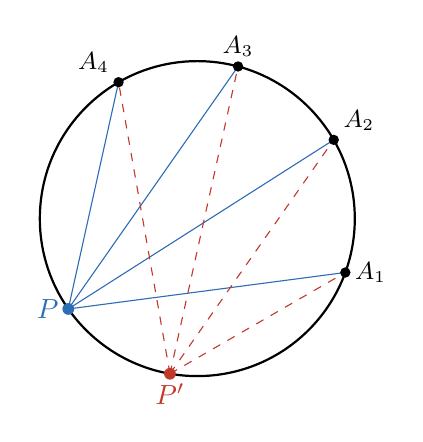
\begin{tikzpicture}[scale=1.25]
  \draw[thick] (0,0) circle (1.6);
  \foreach \a/\i in {-20/1,30/2,75/3,120/4}{\coordinate (A\i) at (\a:1.6);}
  \coordinate (P) at (215:1.6); \coordinate (Q) at (260:1.6);
  \foreach \i in {1,2,3,4}{\draw[figblue] (P)--(A\i); \draw[figred,dashed] (Q)--(A\i);}
  \foreach \i/\pos in {1/right,2/above right,3/above,4/above left}{\fill (A\i) circle (1.5pt) node[\pos] {\small $A_\i$};}
  \fill[figblue] (P) circle (1.7pt) node[left,figblue] {$P$};
  \fill[figred] (Q) circle (1.7pt) node[below,figred] {$P'$};
\end{tikzpicture}
\caption{同弧所对圆周角相等 $\Rightarrow$ 两组连线的夹角相同 $\Rightarrow$ 交比相同}
\end{figure}

\zheng 由圆周角定理（用有向角写，模 $180^\circ$）：对圆上任意一点 $P\neq A_i,A_j$，
\[
\langle PA_i,PA_j\rangle\equiv\tfrac12\angle A_iOA_j\pmod{180^\circ}
\]
（$O$ 为圆心），即这些角与 $P$ 无关。由第 8 题，$(PA_1,PA_2;PA_3,PA_4)$ 只由 $\langle PA_1,PA_3\rangle$、$\langle PA_3,PA_2\rangle$、$\langle PA_1,PA_4\rangle$、$\langle PA_4,PA_2\rangle$ 决定，而第 8 题后面已说明公式对“模 $180^\circ$”良定义，所以交比与 $P$ 无关。\qed

\begin{intbox}{伏笔}
这就是 \S7.6 \key{Steiner 定理}在圆上的特例：对任意非退化二次曲线（椭圆、双曲线、抛物线都是圆的射影像），从曲线上一点看四个定点的交比都是常数。
\end{intbox}

% ================= §7.4 射影坐标和射影坐标变换 =================
\Needspace{12\baselineskip}
\section{射影坐标和射影坐标变换}

\S7.1 的齐次坐标借用了欧氏平面上的仿射标架 $[O_1;\vv d_1,\vv d_2]$。我们希望\key{直接用射影平面上的“点”做标架}。

\subsection{点的射影坐标}

先在把 $O$ 里想：取仿射标架 $[O;\vv d_1,\vv d_2,\vv d_3]$，把中每条直线就有了坐标（方向向量的坐标，差一个倍数）。但“点”只是直线，\key{方向向量的长度没有意义}：三条基本直线 $l_1,l_2,l_3$ 只确定 $\vv d_i$ 的方向，各自的倍数无法确定——这时坐标就不唯一了。

\key{补救办法}：再取一条直线 $l_4$，规定 $\vv d=\vv d_1+\vv d_2+\vv d_3$ 是 $l_4$ 的方向向量。若换取 $\vv d'=\lambda\vv d$，$\vv d_i'=\lambda_i\vv d_i$ 且 $\vv d'=\sum\vv d_i'$，比较系数得 $\lambda_1=\lambda_2=\lambda_3=\lambda$——各基向量的倍数被\key{统一}了，坐标只差一个公共倍数。

\begin{defbox}{定义 4.1–4.2（射影标架与射影坐标）}
$\pib$ 上取\key{一般位置的四个点}（任三点不共线）$A_1,A_2,A_3,E$。取各点对应的向量 $\vv a_1,\vv a_2,\vv a_3,\vv e$，并调整倍数使
\[
\vv e=\vv a_1+\vv a_2+\vv a_3 .
\]
若点 $M$ 对应 $\vv m=x_1\vv a_1+x_2\vv a_2+x_3\vv a_3$，则 $(x_1,x_2,x_3)\T$ 称为 $M$ 在\key{基底} $[A_1,A_2,A_3,E]$ 中的（齐次）\key{射影坐标}。$A_1,A_2,A_3$ 叫\key{基本点}，坐标 $(1,0,0)\T,(0,1,0)\T,(0,0,1)\T$；$E$ 叫\key{单位点}，坐标 $(1,1,1)\T$；$\triangle A_1A_2A_3$ 叫\key{坐标三角形}。
\end{defbox}

\begin{gdbox}{高代联动：为什么射影标架要 4 个点}
线性空间 $\R^3$ 的基是 3 个向量。但射影平面的“点”只是 1 维子空间，3 个点只给出 3 条“基向量所在的直线”，基向量可以各自伸缩——相当于基 $\{\vv a_1,\vv a_2,\vv a_3\}$ 只确定到 $\operatorname{diag}(k_1,k_2,k_3)$。第四个点 $E$（“单位点”）规定 $\vv e=\vv a_1+\vv a_2+\vv a_3$，把 $k_1=k_2=k_3$ 强制统一，剩下的公共倍数正是齐次坐标本来就允许的。一句话：\key{射影标架 = 基 + 比例尺}。
\end{gdbox}

\begin{figure}[htbp]
\centering
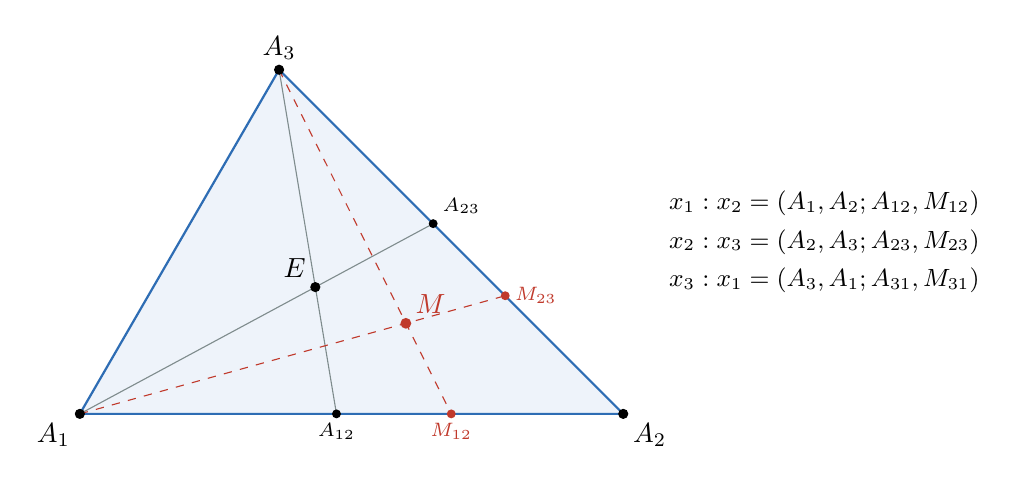
\begin{tikzpicture}[scale=1.15]
  \coordinate (A1) at (0,0); \coordinate (A2) at (6,0); \coordinate (A3) at (2.2,3.8);
  \coordinate (E) at (2.6,1.4); \coordinate (M) at (3.6,1.0);
  \coordinate (A12) at (intersection of A3--E and A1--A2);
  \coordinate (M12) at (intersection of A3--M and A1--A2);
  \coordinate (A23) at (intersection of A1--E and A2--A3);
  \coordinate (M23) at (intersection of A1--M and A2--A3);
  \fill[defbg] (A1)--(A2)--(A3)--cycle;
  \draw[thick,defblue] (A1)--(A2)--(A3)--cycle;
  \draw[figgray] (A3)--(A12) (A1)--(A23);
  \draw[figred,dashed] (A3)--(M12) (A1)--(M23);
  \foreach \p/\l/\pos in {A1/A_1/below left,A2/A_2/below right,A3/A_3/above}{\fill (\p) circle (1.6pt) node[\pos] {$\l$};}
  \fill (E) circle (1.6pt) node[above left] {$E$};
  \fill[figred] (M) circle (1.7pt) node[above right,figred] {$M$};
  \fill (A12) circle (1.4pt) node[below] {\scriptsize $A_{12}$};
  \fill[figred] (M12) circle (1.4pt) node[below,figred] {\scriptsize $M_{12}$};
  \fill (A23) circle (1.4pt) node[above right] {\scriptsize $A_{23}$};
  \fill[figred] (M23) circle (1.4pt) node[right,figred] {\scriptsize $M_{23}$};
  \node[align=left,right] at (6.4,1.9) {\small $x_1:x_2=(A_1,A_2;A_{12},M_{12})$\\[2pt]\small $x_2:x_3=(A_2,A_3;A_{23},M_{23})$\\[2pt]\small $x_3:x_1=(A_3,A_1;A_{31},M_{31})$};
\end{tikzpicture}
\caption{射影坐标的几何意义：坐标之比都是交比（$A_{12}=A_3E\cap A_1A_2$，$M_{12}=A_3M\cap A_1A_2$，……）}
\end{figure}

\begin{thmbox}{射影坐标的几何意义与两点注意}
\begin{itemize}
\item 对不在坐标三角形边上的点 $M$：$x_1:x_2=(A_1,A_2;A_{12},M_{12})$ 等（见上图），所以射影坐标\key{与 $O$ 的取法无关}，是射影平面自身的概念。
\item \S7.1 的齐次（仿射）坐标是\key{特殊基底}：$A_1,A_2$ 是 $x,y$ 轴的无穷远点，$A_3$ 是原点，$E$ 是点 $(1,1)$。
\item 一般基底下，\key{不能用 $x_3=0$ 判断无穷远点}——射影坐标根本“看不见”哪条线是无穷远直线。
\end{itemize}
\end{thmbox}

\subsection{射影坐标变换公式}

设两个基底 I$[A_1,A_2,A_3,E]$ 和 II$[A_1',A_2',A_3',E']$，点 $M$ 的 I 坐标 $X=(x_1,x_2,x_3)\T$，II 坐标 $X'$。则
\begin{equation}
\rho X=HX',\qquad \rho\neq0,\ |H|\neq0,
\end{equation}
其中 $H$ 的第 $j$ 列是 $\lambda_j\times(A_j'$ 的 I 坐标$)$，$\lambda_j$ 由
\[
\lambda\,(E'\text{ 的 I 坐标})=\lambda_1(A_1'\text{ 的 I 坐标})+\lambda_2(A_2'\text{ 的 I 坐标})+\lambda_3(A_3'\text{ 的 I 坐标})
\]
确定（与线性代数的“过渡矩阵的列 = 新基在旧基下的坐标”完全一样，只是新基向量的倍数要用 $E'$ 来校准）。

\begin{mtbox}{求射影坐标变换的三步法}
\textbf{①} 写出 $A_1',A_2',A_3',E'$ 的 I 坐标 $\vv a_1',\vv a_2',\vv a_3',\vv e'$；\quad
\textbf{②} 解 $\vv e'=\lambda_1\vv a_1'+\lambda_2\vv a_2'+\lambda_3\vv a_3'$（即解 $(\vv a_1',\vv a_2',\vv a_3')\vv\lambda=\vv e'$）；\\
\textbf{③} $H=(\lambda_1\vv a_1',\ \lambda_2\vv a_2',\ \lambda_3\vv a_3')$，得 $\rho X=HX'$。\\[2pt]
\textbf{检验}：$H(1,1,1)\T=\vv e'$；$\lambda_j$ 全不为零 $\iff$ 四点一般位置（某个 $\lambda_j=0$ 说明 $E'$ 落在坐标三角形的边上）。
\end{mtbox}

\begin{mtbox}{例 4.1}
$A_1',A_2',A_3',E'$ 的 I 坐标为 $(1,-1,2)\T,(2,0,1)\T,(-1,2,4)\T,(1,-1,0)\T$。解
\[
\lambda(1,-1,0)\T=\lambda_1(1,-1,2)\T+\lambda_2(2,0,1)\T+\lambda_3(-1,2,4)\T
\]
得 $\lambda_1=\frac7{15}\lambda,\ \lambda_2=\frac2{15}\lambda,\ \lambda_3=-\frac4{15}\lambda$，取 $\lambda=15$：$\lambda_1=7,\lambda_2=2,\lambda_3=-4$。于是
\[
\rho\begin{pmatrix}x_1\\x_2\\x_3\end{pmatrix}=\begin{pmatrix}7&4&4\\-7&0&-8\\14&2&-16\end{pmatrix}\begin{pmatrix}x_1'\\x_2'\\x_3'\end{pmatrix}.
\]
检验：$H(1,1,1)\T=(15,-15,0)\T\sim(1,-1,0)\T=E'$。\checkmark
\end{mtbox}

\subsection{直线的射影坐标方程、用射影坐标计算交比}
与 \S7.1 完全一样：直线 $PQ$ 的参数方程 $\vv x=\lambda\vv p+\mu\vv q$，方程 $\eta_1x_1+\eta_2x_2+\eta_3x_3=0$（$\vv\eta=\vv p\times\vv q$），三点共线 $\iff$ 行列式 $=0$。

\begin{thmbox}{定理 4.1（交比公式在任意射影坐标下成立）}
在任一基底中，若 $\vv c=\lambda_1\vv a+\mu_1\vv b$，$\vv d=\lambda_2\vv a+\mu_2\vv b$，则 $(A,B;C,D)=\dfrac{\lambda_2}{\mu_2}\Big/\dfrac{\lambda_1}{\mu_1}$。
\end{thmbox}
\noindent\textbf{理由}：换到一个使公式已知成立的基底 II（$B_1,B_2$ 为无穷远点，即齐次坐标），坐标变换 $\rho X=HX'$ 是线性的，$\vv c=\lambda_1\vv a+\mu_1\vv b$ 变成 $\rho_3^{-1}H\vv c'=\lambda_1\rho_1^{-1}H\vv a'+\mu_1\rho_2^{-1}H\vv b'$，系数比 $\lambda_1/\mu_1$ 只多出因子 $\rho_2/\rho_1$，对 $D$ 也多出同一个因子，相除抵消。

\subsection{点的非齐次射影坐标}
对不在 $A_1A_2$ 上的点，令 $x=\frac{x_1}{x_3},\ y=\frac{x_2}{x_3}$，称为\key{非齐次射影坐标}（它们就是交比：$x=(A_1,A_3;A_{13},M_{13})$，$y=(A_2,A_3;A_{23},M_{23})$）。两个基底间的变换是\key{分式线性函数}：
\begin{equation}
x=\frac{a_{11}x'+a_{12}y'+a_{13}}{a_{31}x'+a_{32}y'+a_{33}},\qquad
y=\frac{a_{21}x'+a_{22}y'+a_{23}}{a_{31}x'+a_{32}y'+a_{33}}.
\end{equation}

\begin{intbox}{直觉：分母就是“地平线”}
仿射坐标变换的分母恒为 1；射影坐标变换多了分母 $a_{31}x'+a_{32}y'+a_{33}$。分母为零的那条直线被送到“无穷远”——这就是照片里的地平线。手机“文档扫描”把斜拍的纸张拉正，用的正是这种分式线性变换（\S7.5）。
\end{intbox}

% ---------------- 习题 7.4 ----------------
\xiti{7.4}

\begin{ex}{7.4.1}
设在射影平面的一个基底 I 中给定了点 $B_1(4,-2,3)\T$，$B_2(5,2,0)\T$，$B_3(1,3,-2)\T$，$F(1,1,0)\T$，$M(1,1,-1)\T$，证明点 $B_1,B_2,B_3,F$ 是一般位置的四个点，并且求基底 I 到基底 II$[B_1,B_2,B_3,F]$ 的射影坐标变换公式，以及 $M$ 在基底 II 中的射影坐标。
\end{ex}
\jie \textbf{一般位置}：$|\vv b_1,\vv b_2,\vv b_3|=\begin{vmatrix}4&5&1\\-2&2&3\\3&0&-2\end{vmatrix}=3\neq0$，三基本点不共线。解 $\vv f=\lambda_1\vv b_1+\lambda_2\vv b_2+\lambda_3\vv b_3$：
\[
\begin{cases}4\lambda_1+5\lambda_2+\lambda_3=1\\-2\lambda_1+2\lambda_2+3\lambda_3=1\\3\lambda_1-2\lambda_3=0\end{cases}
\Rightarrow\ \lambda_1=2,\ \lambda_2=-2,\ \lambda_3=3 .
\]
三个 $\lambda$ 都不为零，$F$ 不在坐标三角形的边上，所以四点是一般位置。

\textbf{变换公式}：$H=(2\vv b_1,-2\vv b_2,3\vv b_3)$，
\[
\rho\begin{pmatrix}x_1\\x_2\\x_3\end{pmatrix}=\begin{pmatrix}8&-10&3\\-4&-4&9\\6&0&-6\end{pmatrix}\begin{pmatrix}x_1'\\x_2'\\x_3'\end{pmatrix}.
\]
\textbf{$M$ 的 II 坐标}：解 $HX'=(1,1,-1)\T$，得 $X'=-\frac16(7,8,6)\T$，即 $M$ 的 II 坐标为 $(7,8,6)\T$。检验：$H(7,8,6)\T=(-6,-6,6)\T\sim(1,1,-1)\T$。\checkmark

\begin{ex}{7.4.2}
在射影平面上，求基底 I$[A_1,A_2,A_3,E]$ 到基底 II$[A_3,A_1,E,A_2]$ 的射影坐标变换公式。
\end{ex}
\jie 新基底的四个点在 I 中的坐标：$A_1'=A_3=(0,0,1)\T$，$A_2'=A_1=(1,0,0)\T$，$A_3'=E=(1,1,1)\T$，$E'=A_2=(0,1,0)\T$。解
\[
(0,1,0)\T=\lambda_1(0,0,1)\T+\lambda_2(1,0,0)\T+\lambda_3(1,1,1)\T\ \Rightarrow\ \lambda_3=1,\ \lambda_2=-1,\ \lambda_1=-1 .
\]
所以
\[
\rho\begin{pmatrix}x_1\\x_2\\x_3\end{pmatrix}=\begin{pmatrix}0&-1&1\\0&0&1\\-1&0&1\end{pmatrix}\begin{pmatrix}x_1'\\x_2'\\x_3'\end{pmatrix}
\quad\Big(\text{与教材答案 }\begin{pmatrix}0&1&-1\\0&0&-1\\1&0&-1\end{pmatrix}\text{ 只差因子 }-1\Big).
\]
检验：$X'=(1,1,1)\T$（II 的单位点）$\mapsto X=(0,1,0)\T=A_2$。\checkmark

\begin{ex}{7.4.3}
在射影平面上，设点 $F$ 在基底 I$[A_1,A_2,A_3,E]$ 中的射影坐标为 $(\varepsilon_1,\varepsilon_2,\varepsilon_3)\T$，并且 $A_1,A_2,A_3,F$ 是一般位置的四个点，求基底 I 到基底 II$[A_1,A_2,A_3,F]$ 的射影坐标变换公式。
\end{ex}
\jie 基本点不变，只换单位点。$\vv f=\varepsilon_1\vv a_1+\varepsilon_2\vv a_2+\varepsilon_3\vv a_3$，所以 $\lambda_j=\varepsilon_j$：
\[
\rho X=\operatorname{diag}(\varepsilon_1,\varepsilon_2,\varepsilon_3)\,X' .
\]
一般位置保证 $\varepsilon_1\varepsilon_2\varepsilon_3\neq0$。\key{直觉}：换单位点 = 三个基向量各自伸缩——对角矩阵。

\begin{ex}{7.4.4}
在射影平面上取四点 $B_1(1,2,1)\T,B_2(1,1,0)\T,B_3(2,1,1)\T,F(0,1,7)\T$，求点 $M(1,1,1)\T$ 在基底 $[B_1,B_2,B_3,F]$ 中的坐标。
\end{ex}
\jie $|\vv b_1,\vv b_2,\vv b_3|=-2\neq0$。解 $\vv f=\lambda_1\vv b_1+\lambda_2\vv b_2+\lambda_3\vv b_3$ 得 $\lambda_1=4,\lambda_2=-10,\lambda_3=3$（验：$4(1,2,1)-10(1,1,0)+3(2,1,1)=(0,1,7)$）。于是
\[
\rho X=\begin{pmatrix}4&-10&6\\8&-10&3\\4&0&3\end{pmatrix}X' .
\]
解 $HX'=(1,1,1)\T$ 得 $X'=(\frac18,\frac1{20},\frac16)\T\sim(15,6,20)\T$。检验：$H(15,6,20)\T=(120,120,120)\T$。\checkmark

\begin{ex}{7.4.5}
证明 Pappus（帕普斯）定理：设 $A,B,C$；$A',B',C'$ 分别是直线 $l_1$ 和 $l_2$ 上的三个点，并且均与 $l_1$ 和 $l_2$ 的交点 $D$ 不重合，又设 $AB'$ 与 $A'B$ 交于点 $P$，$BC'$ 与 $B'C$ 交于点 $Q$，$CA'$ 与 $C'A$ 交于点 $R$，则 $P,Q,R$ 三点共线。
\end{ex}

\begin{figure}[htbp]
\centering
\begin{tikzpicture}[scale=1.05]
  \coordinate (A) at (0.6,0); \coordinate (B) at (3.0,0); \coordinate (C) at (6.2,0);
  \coordinate (A') at (0.9,2.9); \coordinate (B') at (3.9,3.1); \coordinate (C') at (5.8,3.24);
  \draw[thick] (-0.3,0)--(7,0) node[right] {$l_1$};
  \draw[thick] (-0.3,2.82)--(7,3.32) node[right] {$l_2$};
  \draw[figblue] (A)--(B') (B)--(A');
  \draw[figred] (B)--(C') (C)--(B');
  \draw[figgreen!70!black] (C)--(A') (A)--(C');
  \coordinate (P) at (intersection of A--B' and A'--B);
  \coordinate (Q) at (intersection of B--C' and B'--C);
  \coordinate (R) at (intersection of C--A' and C'--A);
  \draw[keyred,very thick] ($(P)!-0.15!(Q)$)--($(P)!1.25!(Q)$);
  \foreach \p/\pos in {A/below,B/below,C/below,A'/above,B'/above,C'/above}{\fill (\p) circle (1.6pt) node[\pos] {$\p$};}
  \foreach \p in {P,Q,R}{\fill[keyred] (\p) circle (2pt) node[below=2pt,keyred] {$\p$};}
  \node[keyred] at ($(P)!1.36!(Q)+(0,0.1)$) {\small Pappus 线};
\end{tikzpicture}
\caption{Pappus 定理：两条直线上各三点“交叉连线”的三个交点共线}
\end{figure}

\zheng 取基底 $[O_1,O_2,D,E]$，其中 $O_1\in l_1$、$O_2\in l_2$ 与六个点都不同，$E$ 为一般位置的点。于是 $O_1=(1,0,0)\T$，$O_2=(0,1,0)\T$，$D=(0,0,1)\T$，$l_1=O_1D:\ x_2=0$，$l_2=O_2D:\ x_1=0$。$l_1$ 上异于 $D$ 的点可写成 $(1,0,t)\T$，$l_2$ 上的写成 $(0,1,t)\T$：
\[
A(1,0,a),\ B(1,0,b),\ C(1,0,c);\qquad A'(0,1,a'),\ B'(0,1,b'),\ C'(0,1,c').
\]
用叉积：$AB'=(-a,-b',1)\T$，$A'B=(b,a',-1)\T$，
\[
\vv p=AB'\times A'B=(b'-a',\ b-a,\ bb'-aa')\T .
\]
把 $(A,B)$ 依次换成 $(B,C)$、$(C,A)$ 得
\[
\vv q=(c'-b',\ c-b,\ cc'-bb')\T,\qquad \vv r=(a'-c',\ a-c,\ aa'-cc')\T .
\]
显然 $\vv p+\vv q+\vv r=\vv0$（每个分量都是“循环差”之和），三向量线性相关，$P,Q,R$ 共线。\qed

\begin{intbox}{直觉}
和 Desargues 的证明一样，结论又是“三个向量之和为零”。选 $D$ 为基本点、两条直线为坐标三角形的两边，是把“两条直线”的条件吃进坐标里的标准手法。（把 $l_1\cup l_2$ 看成一条退化的二次曲线，Pappus 就是 \S7.6 Pascal 定理的退化情形。）
\end{intbox}

\begin{ex}{7.4.6}
在射影平面上取一个基底 $[A_1,A_2,A_3,E]$，设 $A_{23}$ 是直线 $A_1E$ 与 $A_2A_3$ 的交点，求直线 $A_2A_3$ 上的一个点 $P$，使得交比 $(A_2,A_3;A_{23},P)=a$。
\end{ex}
\jie $A_1E:\ x_2=x_3$，$A_2A_3:\ x_1=0$，所以 $A_{23}=(0,1,1)\T=\vv a_2+\vv a_3$（$\frac{\lambda_1}{\mu_1}=1$）。设 $P=\lambda\vv a_2+\mu\vv a_3$，由定理 4.1，$\frac{\lambda}{\mu}\big/1=a$，取 $\lambda=a,\mu=1$：
\[
P=(0,a,1)\T .
\]
这也正是“非齐次射影坐标就是交比”的一个具体例子：$A_2A_3$ 上点 $(0,x_2,x_3)$ 的 $x_2:x_3$ 就等于 $(A_2,A_3;A_{23},P)$。

\begin{ex}{7.4.7}
在射影平面上给了一个三角形 $A_1A_2A_3$，设 $P_1,P_2,P_3$ 分别在直线 $A_2A_3,A_3A_1,A_1A_2$ 上，但是都不和 $A_1,A_2,A_3$ 重合，而 $Q_1,Q_2,Q_3$ 依次为 $P_1,P_2,P_3$ 对于 $A_2,A_3$；$A_3,A_1$；$A_1,A_2$ 的调和共轭点，证明：$A_1Q_1,A_2Q_2,A_3Q_3$ 共点的充分必要条件是 $P_1,P_2,P_3$ 共线。
\end{ex}

\begin{figure}[htbp]
\centering
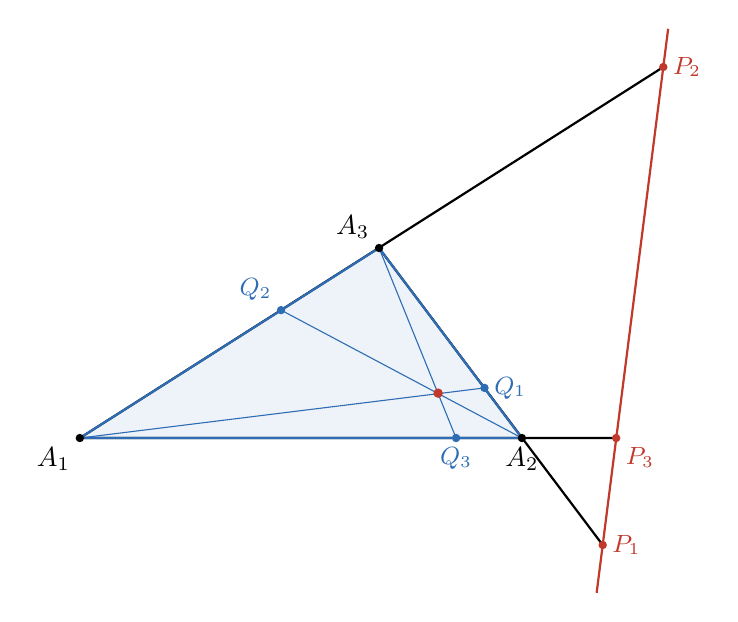
\begin{tikzpicture}[scale=0.95]
  \coordinate (A1) at (0,0); \coordinate (A2) at (5.91,0); \coordinate (A3) at (4.0,2.54);
  \coordinate (O) at (4.79,0.6);
  \coordinate (Q1) at (5.41,0.67); \coordinate (Q2) at (2.69,1.71); \coordinate (Q3) at (5.03,0);
  \coordinate (P1) at (6.99,-1.43); \coordinate (P2) at (7.8,4.96); \coordinate (P3) at (7.17,0);
  \fill[defbg] (A1)--(A2)--(A3)--cycle;
  \draw[thick] (A1)--(P3) (A3)--(P1) (A1)--(P2);
  \draw[defblue,thick] (A1)--(A2)--(A3)--cycle;
  \draw[figblue] (A1)--(Q1) (A2)--(Q2) (A3)--(Q3);
  \draw[figred,thick] ($(P1)!-0.1!(P2)$)--($(P1)!1.08!(P2)$);
  \foreach \p/\l/\pos in {A1/A_1/below left,A2/A_2/below,A3/A_3/above left}{\fill (\p) circle (1.6pt) node[\pos] {$\l$};}
  \foreach \p/\l/\pos in {Q1/Q_1/right,Q2/Q_2/above left,Q3/Q_3/below}{\fill[figblue] (\p) circle (1.6pt) node[\pos,figblue] {\small $\l$};}
  \foreach \p/\l/\pos in {P1/P_1/right,P2/P_2/right,P3/P_3/below right}{\fill[figred] (\p) circle (1.6pt) node[\pos,figred] {\small $\l$};}
  \fill[keyred] (O) circle (1.8pt);
\end{tikzpicture}
\caption{$P_i$ 共线（红） $\iff$ 它们的调和共轭点 $Q_i$ 与对顶点的连线共点（蓝）}
\end{figure}

\zheng 取基底 $[A_1,A_2,A_3,E]$（$E$ 任取一般位置点）。设
\[
P_1=\vv a_2+t_1\vv a_3=(0,1,t_1)\T,\quad P_2=\vv a_3+t_2\vv a_1=(t_2,0,1)\T,\quad P_3=\vv a_1+t_3\vv a_2=(1,t_3,0)\T,
\]
$t_i\neq0$（不与顶点重合）。$P_1=1\cdot\vv a_2+t_1\vv a_3$，其调和共轭点为 $Q_1=\vv a_2-t_1\vv a_3$（系数比变号，交比 $=-1$）。同理
\[
Q_1=(0,1,-t_1)\T,\qquad Q_2=(-t_2,0,1)\T,\qquad Q_3=(1,-t_3,0)\T .
\]
\textbf{$P_i$ 共线}：$\begin{vmatrix}0&1&t_1\\t_2&0&1\\1&t_3&0\end{vmatrix}=1+t_1t_2t_3=0$。

\textbf{$A_iQ_i$ 共点}：三条线坐标 $A_1Q_1=(0,t_1,1)\T$，$A_2Q_2=(1,0,t_2)\T$，$A_3Q_3=(t_3,1,0)\T$，
\[
\begin{vmatrix}0&t_1&1\\1&0&t_2\\t_3&1&0\end{vmatrix}=1+t_1t_2t_3=0 .
\]
两个条件都是 $t_1t_2t_3=-1$，所以等价。\qed

\begin{intbox}{几何意义}
若 $P_1P_2P_3$ 是无穷远直线，则 $Q_i$ 是\key{各边中点}（中点 $\leftrightarrow$ 无穷远点调和共轭），结论变成“\key{三角形三条中线共点}”。一般情形是它的射影像：任意一条直线都可以被射影变换送到无穷远。
\end{intbox}

\begin{ex}{7.4.8}
在射影平面上，设 $A_1,A_2,A_3$ 和 $P_1,P_2,P_3$ 的意义同第 7 题，但是 $(A_2,A_3;Q_1,P_1)=e_1,\ (A_3,A_1;Q_2,P_2)=e_2,\ (A_1,A_2;Q_3,P_3)=e_3$，证明：若 $P_1,P_2,P_3$ 共线，则 $Q_1,Q_2,Q_3$ 共线的充分必要条件是 $e_1e_2e_3=1$。又如果 $P_1,P_2,P_3$ 在扩大的欧氏平面的无穷远直线上，那么上述命题的几何意义是什么？
\end{ex}
\zheng 沿用第 7 题的坐标，$P_1=\vv a_2+t_1\vv a_3$。设 $Q_1=\vv a_2+s_1\vv a_3$，则
\[
e_1=(A_2,A_3;Q_1,P_1)=\frac{1/t_1}{1/s_1}=\frac{s_1}{t_1},\quad\text{即}\quad s_1=e_1t_1;\qquad\text{同理 } s_2=e_2t_2,\ s_3=e_3t_3 .
\]
$Q_1=(0,1,s_1)\T,Q_2=(s_2,0,1)\T,Q_3=(1,s_3,0)\T$ 与 $P_i$ 同形，所以 $Q_i$ 共线 $\iff 1+s_1s_2s_3=0$。已知 $P_i$ 共线，$t_1t_2t_3=-1$，于是
\[
1+s_1s_2s_3=1+e_1e_2e_3\,t_1t_2t_3=1-e_1e_2e_3=0\iff e_1e_2e_3=1.\qquad\blacksquare
\]
\textbf{几何意义}：$P_i$ 在无穷远直线上时，$(A_2,A_3,P_1)=-1$，
\[
e_1=\frac{(A_2,A_3,Q_1)}{(A_2,A_3,P_1)}=-\frac{A_2Q_1}{Q_1A_3},\ \text{等},
\qquad e_1e_2e_3=1\iff \frac{A_2Q_1}{Q_1A_3}\cdot\frac{A_3Q_2}{Q_2A_1}\cdot\frac{A_1Q_3}{Q_3A_2}=-1,
\]
这就是 \key{Menelaus（梅涅劳斯）定理}（第一章 \S2）：三边（所在直线）上的三点共线的充要条件。

\begin{ex}{7.4.9}
在射影平面上，设 $A_1,A_2,A_3,P_1,P_2,P_3,Q_1,Q_2,Q_3$ 的意义同第 8 题，证明：若 $P_1,P_2,P_3$ 共线，则 $A_1Q_1,A_2Q_2,A_3Q_3$ 共点的充分必要条件是 $e_1e_2e_3=-1$。又如果 $P_1,P_2,P_3$ 在扩大的欧氏平面的无穷远直线上，那么上述命题的几何意义是什么？
\end{ex}
\zheng 线坐标 $A_1Q_1=\vv a_1\times\vv q_1=(0,-s_1,1)\T$，$A_2Q_2=(1,0,-s_2)\T$，$A_3Q_3=(-s_3,1,0)\T$，
\[
\begin{vmatrix}0&-s_1&1\\1&0&-s_2\\-s_3&1&0\end{vmatrix}=1-s_1s_2s_3 .
\]
共点 $\iff s_1s_2s_3=1\iff e_1e_2e_3\,t_1t_2t_3=1\iff -e_1e_2e_3=1\iff e_1e_2e_3=-1$。\qed

（第 7 题是 $e_1=e_2=e_3=-1$ 的特例，乘积 $=-1$，吻合。）

\textbf{几何意义}：$P_i$ 在无穷远直线上时，$e_1e_2e_3=-1\iff\frac{A_2Q_1}{Q_1A_3}\cdot\frac{A_3Q_2}{Q_2A_1}\cdot\frac{A_1Q_3}{Q_3A_2}=1$，这是 \key{Ceva（塞瓦）定理}（习题 2.3 第 12 题）。

\begin{ckbox}{对照：Menelaus 与 Ceva 是一对“射影孪生”}
同一个三角形、同样的分比 $\frac{A_2Q_1}{Q_1A_3}$，乘积 $=-1$ 是三点共线，$=+1$ 是三线共点。射影观点下差别仅在 $e_1e_2e_3=\pm1$。
\end{ckbox}

\begin{ex}{7.4.10$^*$}
射影平面 $\pib$ 上，由一般位置的四个点 $A,B,C,D$（称它们为顶点）和由它们两两相连的六条直线（称它们为边）构成的图形称为\key{完备四点形}，其中不在同一顶点上的两条边称为对边，对边的交点称为\key{对角点}，如图中的 $E,F,G$ 均是对角点。(1) 证明：完备四点形的三个对角点不共线。由这三个对角点确定的三角形称为完备四点形的\key{对角三角形}。(2) 证明：完备四点形的任意两个对角点调和分割它们的连线和另外两条边的交点。
\end{ex}

\begin{figure}[htbp]
\centering
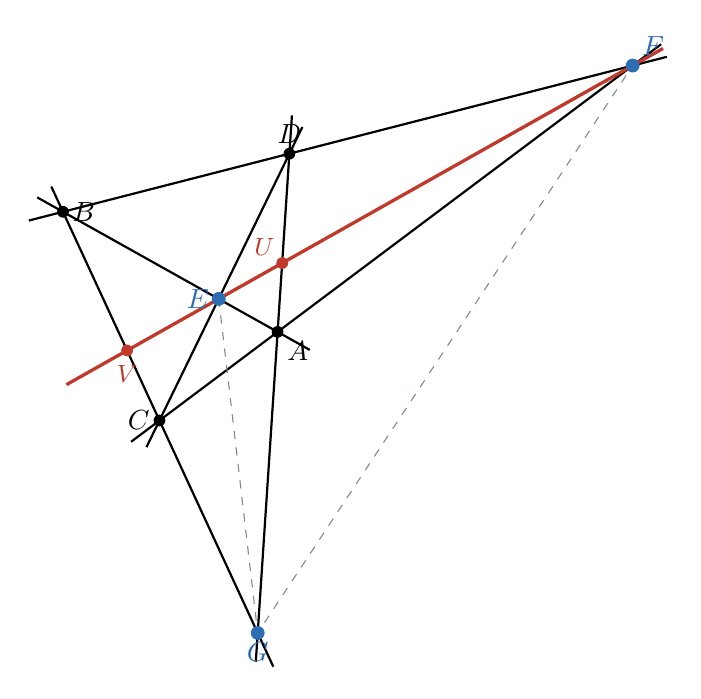
\begin{tikzpicture}[scale=1.25]
  \coordinate (A) at (2.67,1.66); \coordinate (B) at (0.49,2.88); \coordinate (C) at (1.47,0.76); \coordinate (D) at (2.79,3.47);
  \coordinate (E) at (intersection of A--B and C--D);
  \coordinate (F) at (intersection of A--C and B--D);
  \coordinate (G) at (intersection of A--D and B--C);
  \coordinate (U) at (intersection of E--F and A--D);
  \coordinate (V) at (intersection of E--F and B--C);
  \draw[thick] ($(B)!-0.12!(A)$)--($(B)!1.15!(A)$);   % AB
  \draw[thick] ($(C)!-0.1!(D)$)--($(C)!1.1!(D)$);     % CD
  \draw[thick] ($(C)!-0.06!(F)$)--($(C)!1.06!(F)$);   % AC
  \draw[thick] ($(B)!-0.06!(F)$)--($(B)!1.06!(F)$);   % BD
  \draw[thick] ($(G)!-0.06!(D)$)--($(G)!1.08!(D)$);   % AD
  \draw[thick] ($(B)!-0.06!(G)$)--($(B)!1.08!(G)$);   % BC
  \draw[figred,very thick] ($(V)!-0.12!(F)$)--($(V)!1.06!(F)$);
  \draw[figgray,dashed] (E)--(G)--(F);
  \foreach \p/\pos in {A/below right,B/right,C/left,D/above}{\fill (\p) circle (1.7pt) node[\pos] {$\p$};}
  \foreach \p/\pos in {E/left,F/above right,G/below}{\fill[figblue] (\p) circle (2pt) node[\pos,figblue] {$\p$};}
  \fill[figred] (U) circle (1.7pt) node[above left=-1pt,figred] {\small $U$};
  \fill[figred] (V) circle (1.7pt) node[below=2pt,figred] {\small $V$};
\end{tikzpicture}
\caption{完备四点形 $ABCD$，对角点 $E,F,G$（蓝），$(E,F;U,V)=-1$}
\end{figure}

\zheng 取基底 $[A,B,C,D]$：$A=(1,0,0)\T,B=(0,1,0)\T,C=(0,0,1)\T,D=(1,1,1)\T$。六条边：
\[
AB:x_3=0,\ CD:x_1=x_2;\quad AC:x_2=0,\ BD:x_1=x_3;\quad AD:x_2=x_3,\ BC:x_1=0 .
\]
对角点：$E=AB\cap CD=(1,1,0)\T$，$F=AC\cap BD=(1,0,1)\T$，$G=AD\cap BC=(0,1,1)\T$。

(1) $\begin{vmatrix}1&1&0\\1&0&1\\0&1&1\end{vmatrix}=-2\neq0$，三个对角点不共线。

(2) 以 $E,F$ 为例（另两种情形同理，或换基底的顶点顺序）。$EF=(1,1,0)\T\times(1,0,1)\T=(1,-1,-1)\T$：$x_1-x_2-x_3=0$。另外两条边是不过 $E,F$ 的 $AD,BC$：
\[
U=EF\cap AD=(2,1,1)\T=\vv e+\vv f,\qquad V=EF\cap BC=(0,1,-1)\T=\vv e-\vv f,
\]
所以 $(E,F;U,V)=\dfrac{1/(-1)}{1/1}=-1$。\qed

\begin{intbox}{有趣的反例：Fano 平面}
(1) 的行列式等于 $-2$。在特征为 2 的域上 $-2=0$——$PG(2,2)$（Fano 平面）中完备四点形的对角点\key{共线}（\S7.1 图中那个“圆”）！所以“对角点不共线”其实依赖于 $1+1\neq0$。
\end{intbox}

\begin{ex}{7.4.11$^*$}
在射影平面上，完备四点形的对偶称为\key{完备四边形}。叙述第 10 题中第 (2) 小题的对偶命题，并且说明调和线束的作图方法。
\end{ex}
\jie\textbf{完备四边形}：一般位置（任三条不共点）的四条直线（边），它们两两的六个交点（顶点）；不在同一条边上的两个顶点叫\key{相对顶点}，三对相对顶点的连线叫\key{对角线}。

\begin{thmbox}{第 10(2) 题的对偶命题}
完备四边形的任意两条对角线，被它们的交点与另外两个顶点（即第三条对角线上的两个顶点）的连线调和分割。也就是：若对角线 $x,y$ 交于 $O$，第三条对角线上的顶点为 $W_1,W_2$，则 $(x,y;OW_1,OW_2)=-1$。
\end{thmbox}

\textbf{调和线束的作图}：已知共点于 $O$ 的三条直线 $l_1,l_2,l_3$，求第四调和线 $l_4$。
\begin{enumerate}
\item 作一条不过 $O$ 的直线 $l$，交 $l_i$ 于 $B_i$（$i=1,2,3$）；
\item 过 $B_3$ 作另一条直线 $l'$，交 $l_1,l_2$ 于 $D_1,D_2$；
\item 连 $D_1B_2$、$D_2B_1$，交于 $D_4$；
\item 直线 $OD_4$ 即为所求 $l_4$。
\end{enumerate}

\begin{figure}[htbp]
\centering
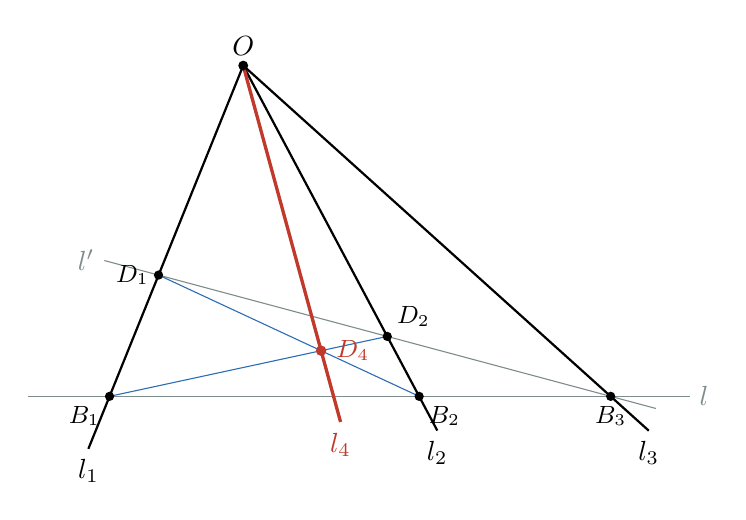
\begin{tikzpicture}[scale=1.05]
  \coordinate (O) at (0,4.2);
  \coordinate (E1) at ($(O)+(-112:5)$); \coordinate (E2) at ($(O)+(-62:5)$); \coordinate (E3) at ($(O)+(-42:6.6)$);
  \coordinate (La) at (-2.6,0.2); \coordinate (Lb) at (5.4,0.2);
  \coordinate (B1) at (intersection of O--E1 and La--Lb);
  \coordinate (B2) at (intersection of O--E2 and La--Lb);
  \coordinate (B3) at (intersection of O--E3 and La--Lb);
  \coordinate (K) at ($(B3)+(165:1)$);
  \coordinate (D1) at (intersection of O--E1 and B3--K);
  \coordinate (D2) at (intersection of O--E2 and B3--K);
  \coordinate (D4) at (intersection of D1--B2 and D2--B1);
  \draw[thick] (O)--(E1) node[below] {$l_1$}; \draw[thick] (O)--(E2) node[below] {$l_2$}; \draw[thick] (O)--(E3) node[below] {$l_3$};
  \draw[figgray] (La)--(Lb) node[right] {$l$};
  \draw[figgray] ($(B3)!-0.1!(D1)$)--($(B3)!1.12!(D1)$) node[left] {$l'$};
  \draw[figblue] (D1)--(B2) (D2)--(B1);
  \draw[figred,very thick] (O)--($(O)!1.25!(D4)$) node[below,figred] {$l_4$};
  \foreach \p/\l/\pos in {B1/B_1/below left,B2/B_2/below right,B3/B_3/below,D1/D_1/left,D2/D_2/above right}{\fill (\p) circle (1.6pt) node[\pos] {\small $\l$};}
  \fill (O) circle (1.7pt) node[above] {$O$};
  \fill[figred] (D4) circle (1.8pt) node[right=2pt,figred] {\small $D_4$};
\end{tikzpicture}
\caption{作第四调和线：$(l_1,l_2;l_3,l_4)=-1$}
\end{figure}

\zheng 看完备四点形 $B_1D_1B_2D_2$（顶点 $B_1,D_1\in l_1$，$B_2,D_2\in l_2$）。它的三个对角点是
\[
B_1D_1\cap B_2D_2=l_1\cap l_2=O,\qquad B_1B_2\cap D_1D_2=l\cap l'=B_3,\qquad B_1D_2\cap B_2D_1=D_4 .
\]
对对角点 $B_3,D_4$ 用第 10(2) 题：直线 $B_3D_4$ 与另外两条边 $B_1D_1=l_1$、$B_2D_2=l_2$ 交于 $Z_1,Z_2$，则 $(B_3,D_4;Z_1,Z_2)=-1$。从 $O$ 投影（$OB_3=l_3$，$OD_4=l_4$，$OZ_1=l_1$，$OZ_2=l_2$）：
\[
(l_3,l_4;l_1,l_2)=-1\ \Rightarrow\ (l_1,l_2;l_3,l_4)=-1 .\qquad\blacksquare
\]
（这正是 \S7.3 “作第四调和点”的对偶作图。）

% ================= §7.5 射影映射和射影变换 =================
\Needspace{12\baselineskip}
\section{射影映射和射影变换}

\subsection{射影映射的定义和性质}

\begin{defbox}{定义 5.1（射影映射、射影变换）}
射影平面 $\mathscr P_1$ 的点集到射影平面 $\mathscr P_2$ 的点集的一个\key{双射}，如果把\key{共线三点映成共线三点}，则称为\key{射影映射}。射影平面到自身的射影映射称为\key{射影变换}。中心投影是射影映射。
\end{defbox}

\begin{thmbox}{性质 1–7}
1. 射影映射的乘积是射影映射。\quad 2. 不共线三点 $\mapsto$ 不共线三点。\quad 3. 逆映射也是射影映射。\\
4. 线 $\mapsto$ 线（于是诱导“线集”之间保持关联的双射）。\quad 5. 一般位置四点 $\mapsto$ 一般位置四点。\\
6. 保持共线四点的交比。\quad 7. 保持共点四线的交比。
\end{thmbox}

性质 2 的证明值得一看：若 $A,B,C$ 不共线而像 $A',B',C'$ 在一条线 $l'$ 上，则对任一点 $M$，过 $M$ 作直线交 $AB,AC$ 于 $P,Q$，由 $M,P,Q$ 共线知 $M'$ 也在 $P'Q'=l'$ 上——整个平面都被映到 $l'$ 上，与满射矛盾。

\begin{thmbox}{射影映射基本定理}
\textbf{定理 5.1}：射影映射 $\tau$ 把一般位置的四点 $A_1,A_2,A_3,E$ 映成一般位置的四点 $A_1',A_2',A_3',E'$，并且任一点 $M$ 在基底 I$[A_1,A_2,A_3,E]$ 中的射影坐标\key{等于}它的像在基底 I$'[A_1',A_2',A_3',E']$ 中的射影坐标。\\[3pt]
\textbf{定理 5.2}：任给两组一般位置的四点 $A_1,A_2,A_3,E$ 与 $A_1',A_2',A_3',E'$，\key{存在唯一}的射影映射把前者依次映成后者。\\[3pt]
\textbf{定理 5.3}：在基底 I、II 下，射影映射的公式为
\begin{equation}
\rho\begin{pmatrix}x_1'\\x_2'\\x_3'\end{pmatrix}=\begin{pmatrix}a_{11}&a_{12}&a_{13}\\a_{21}&a_{22}&a_{23}\\a_{31}&a_{32}&a_{33}\end{pmatrix}\begin{pmatrix}x_1\\x_2\\x_3\end{pmatrix},\qquad |A|\neq0;
\end{equation}
反之，这种形式（$A$ 非奇异）的映射一定是射影映射。
\end{thmbox}

\begin{gdbox}{高代联动：$PGL(3,\R)$，8 个参数}
射影变换 $\leftrightarrow$ 可逆矩阵 $A$，且 $A$ 与 $kA$ 给出同一个变换：射影变换群 $\cong GL(3,\R)/\{kI\}=PGL(3,\R)$，维数 $9-1=8$。一个点的像有 2 个自由度，所以要\key{4 对点}才能定下一个射影变换（$4\times2=8$）——与仿射变换“3 对点”（$6$ 个参数）、平面上的射影直线“3 对点”（$PGL(2)$，3 个参数）对照。
\end{gdbox}

\begin{mtbox}{求射影变换的“两次标准化”法}
要求把 $A,B,C,D$（一般位置）依次映成 $A',B',C',D'$ 的射影变换：
\begin{enumerate}
\item 解 $\vv d=\lambda_1\vv a+\lambda_2\vv b+\lambda_3\vv c$，令 $S=(\lambda_1\vv a,\lambda_2\vv b,\lambda_3\vv c)$——$S$ 把标准基底 $[\vv e_1,\vv e_2,\vv e_3,(1,1,1)\T]$ 映成 $[A,B,C,D]$；
\item 同样由 $A',B',C',D'$ 得 $T$；
\item 所求变换的矩阵为 $T\,S^{-1}$（先用 $S^{-1}$ 拉回标准基底，再用 $T$ 推到目标）。
\end{enumerate}
\end{mtbox}

\begin{mtbox}{例 5.1}
求把 $A(1,0,1)\T,B(2,1,1)\T,C(3,-1,0)\T,D(3,5,2)\T$ 分别映成 $A'(-1,0,3)\T,B'(1,1,3)\T,C'(2,3,8)\T,D'(2,1,-2)\T$ 的射影变换 $\sigma$。\\[2pt]
\textbf{解}：$\vv d=-2\vv a+4\vv b-\vv c$，$S=(-2\vv a,\ 4\vv b,\ -\vv c)$；$\vv d'=-\frac32\vv a'-\frac12\vv b'+\frac12\vv c'$，乘 2 得 $T=(-3\vv a',\ -\vv b',\ \vv c')$。计算 $TS^{-1}$ 并约去公因子得
\[
\lambda\begin{pmatrix}x_1'\\x_2'\\x_3'\end{pmatrix}=\begin{pmatrix}-3&23&-21\\-13&9&13\\-53&-31&125\end{pmatrix}\begin{pmatrix}x_1\\x_2\\x_3\end{pmatrix}.
\]
检验：$A\mapsto(-24,0,72)\T\sim A'$，$B\mapsto(-4,-4,-12)\T\sim B'$，$C\mapsto(-32,-48,-128)\T\sim C'$，$D\mapsto(64,32,-64)\T\sim D'$。\checkmark\\
（教材用转置后解矩阵方程、化简化行阶梯形求 $\lambda_i$，结果相同；“两次标准化”更机械、不易错。）
\end{mtbox}

\paragraph{应用：矫正照片。}航拍时底片 $\pi_1$ 与地面 $\pi_0$ 不平行，像会变形。由基本定理，只要在底片和一张地形图上找出\key{四对}对应点，就唯一确定了矫正所需的射影映射。今天手机“扫描文档”把斜拍的纸拉成矩形，原理完全相同。

\begin{figure}[htbp]
\centering
\begin{tikzpicture}[scale=1.55]
  % left: square grid
  \fill[defbg] (0,0) rectangle (1,1);
  \foreach \t in {0,0.25,0.5,0.75,1}{\draw[defblue] (\t,0)--(\t,1); \draw[defblue] (0,\t)--(1,\t);}
  \node[below] at (0.5,0) {\small 地面上的正方形格子};
  \draw[->,thick] (1.3,0.5)--(2.2,0.5) node[midway,above] {\small $\sigma$};
  % right: image x'=2x/(y+1), y'=2y/(y+1)
  \begin{scope}[xshift=2.5cm]
  \fill[thmbg] (0,0)--(2,0)--(1,1)--(0,1)--cycle;
  \foreach \c in {0,0.25,0.5,0.75,1}{\draw[thmred] ({2*\c},0)--(\c,1);}
  \foreach \d in {0,0.25,0.5,0.75,1}{\pgfmathsetmacro{\yy}{2*\d/(\d+1)}\pgfmathsetmacro{\xx}{2/(\d+1)}\draw[thmred] (0,\yy)--(\xx,\yy);}
  \draw[figgray,dashed] (0,1)--(0,2); \draw[figgray,dashed] (1,1)--(0,2); \draw[figgray,dashed] (0.5,1)--(0,2);
  \draw[figor,dashed] (-0.3,2)--(2.3,2) node[right] {\small 地平线 $y'=2$};
  \fill[figor] (0,2) circle (1.2pt) node[above left] {\small 灭点 $(0,2)$};
  \node[below] at (1,0) {\small 照片上的像};
  \end{scope}
\end{tikzpicture}
\caption{射影变换 $x'=\dfrac{2x}{y+1},\ y'=\dfrac{2y}{y+1}$（矩阵 $\begin{psmallmatrix}2&0&0\\0&2&0\\0&1&1\end{psmallmatrix}$）把正方形格子变成“透视地砖”：竖线汇聚于灭点，横线越远越密}
\end{figure}

\begin{intbox}{直觉}
上图中竖直线 $x=c$ 的像是过 $(2c,0)$ 与 $(c,1)$ 的直线，它们都经过 $(0,2)$；横线 $y=d$ 的像 $y'=\frac{2d}{d+1}$ 间距越来越小。\key{平行性、等距性都没了，但直线仍是直线、交比仍不变}——这就是“射影几何”与“仿射几何”的分界。
\end{intbox}

\subsection{射影变换、不动点与不变直线}
射影平面到自身的射影映射构成\key{射影变换群}，交比是射影不变量。

\begin{thmbox}{二级结论：不动点 = 特征向量}
设 $\sigma:\ \lambda X'=AX$。
\begin{itemize}
\item 点 $X$ 不动 $\iff AX=kX$：\key{不动点}就是 $A$ 的特征向量。
\item 直线 $\vv u\T X=0$ 的像是 $\vv u\T A^{-1}X'=0$，即线坐标 $\vv u\mapsto (A^{-1})\T\vv u$；直线不变 $\iff A\T\vv u=k\vv u$：\key{不变直线}就是 $A\T$ 的特征向量。
\item 属于同一特征值的二维特征子空间 = 一整条\key{逐点不动}的直线。
\end{itemize}
\end{thmbox}

\subsection{分式线性变换}
用非齐次射影坐标 $x=\frac{x_1}{x_3},y=\frac{x_2}{x_3}$ 表达，射影变换是
\begin{equation}
x'=\frac{a_{11}x+a_{12}y+a_{13}}{a_{31}x+a_{32}y+a_{33}},\qquad y'=\frac{a_{21}x+a_{22}y+a_{23}}{a_{31}x+a_{32}y+a_{33}},\qquad |A|\neq0 .
\end{equation}

\begin{thmbox}{二级结论：射影直线上的射影变换}
一条射影直线到自身的射影变换（非齐次坐标）为 $x'=\dfrac{ax+b}{cx+d}$，$ad-bc\neq0$（Möbius 变换），由\key{三对}点唯一确定，求法：令 $(x_1,x_2;x_3,x)=(x_1',x_2';x_3',x')$ 解出 $x'$。\\
\textbf{例}：$0\mapsto1,\ 1\mapsto2,\ \infty\mapsto0$。由 $\infty\mapsto0$ 得 $a=0$，$x'=\frac{b}{cx+d}$；$0\mapsto1$ 得 $b=d$；$1\mapsto2$ 得 $c=-\frac b2$。取 $b=2$：$x'=\dfrac{2}{2-x}$。
\end{thmbox}

\subsection{仿射-射影变换}
把无穷远直线映成无穷远直线的射影变换叫\key{仿射-射影变换}。取 $A_1,A_2$ 为无穷远点的基底（即齐次坐标），$x_3=0$ 上的点映成 $x_3'=0$ 上的点，代入 $(1,0,0)\T,(0,1,0)\T$ 得 $a_{31}=a_{32}=0$，于是 $a_{33}\neq0$，除以 $a_{33}$：
\[
\lambda'\begin{pmatrix}x_1'\\x_2'\\x_3'\end{pmatrix}=\begin{pmatrix}c_{11}&c_{12}&c_{13}\\c_{21}&c_{22}&c_{23}\\0&0&1\end{pmatrix}\begin{pmatrix}x_1\\x_2\\x_3\end{pmatrix}
\ \Longrightarrow\
\begin{cases}x'=c_{11}x+c_{12}y+c_{13}\\y'=c_{21}x+c_{22}y+c_{23}\end{cases},\quad\begin{vmatrix}c_{11}&c_{12}\\c_{21}&c_{22}\end{vmatrix}\neq0 .
\]
限制在 $\pi_0$ 上就是第六章的仿射变换——\key{仿射变换 = 保持无穷远直线的射影变换}。

\begin{figure}[htbp]
\centering
\begin{tikzpicture}[scale=1.0]
  \draw[rounded corners=8pt,thick,figpur,fill=gdbg] (0,0) rectangle (13,5.0);
  \draw[rounded corners=8pt,thick,defblue,fill=defbg] (0.3,0.3) rectangle (9.6,3.9);
  \draw[rounded corners=8pt,thick,figgreen,fill=mtbg] (0.6,0.6) rectangle (6.4,2.85);
  \draw[rounded corners=8pt,thick,thmred,fill=thmbg] (0.9,0.9) rectangle (3.4,2.0);
  \node[thmred,align=center] at (2.15,1.45) {\small\textbf{欧氏（正交）}\\[-1pt]\scriptsize 长度、面积};
  \node[figgreen!70!black,align=left,anchor=west] at (3.6,1.75) {\small\textbf{相似}\\[-1pt]\scriptsize 角度、长度比、圆};
  \node[defblue,align=left,anchor=west] at (6.6,2.05) {\small\textbf{仿射}\\[-1pt]\scriptsize 平行、分比、中点\\[-1pt]\scriptsize 面积比、椭圆/双/抛之分};
  \node[figpur,align=left,anchor=west] at (9.8,2.6) {\small\textbf{射影}\\[-1pt]\scriptsize 共线、共点、交比\\[-1pt]\scriptsize 调和、二次曲线、配极};
  \node[figpur] at (6.5,4.45) {\small 变换群越大 $\Rightarrow$ 不变性质越少（Klein 的 Erlangen 纲领）};
\end{tikzpicture}
\caption{几何的层次：欧氏 $\subset$ 相似 $\subset$ 仿射 $\subset$ 射影（按变换群），不变性质则逐层减少}
\end{figure}

% ---------------- 习题 7.5 ----------------
\xiti{7.5}

\begin{ex}{7.5.1}
在射影平面上，取一个基底 $[A_1,A_2,A_3,E]$，求把点 $B_1(1,0,1)\T$，$B_2(2,0,1)\T$，$B_3(0,1,1)\T$，$F(0,2,1)\T$ 分别映成基点 $A_1,A_2,A_3,E$ 的射影变换 $\sigma$ 的公式。
\end{ex}
\jie \key{先求反方向}：把标准基底映成 $B_1,B_2,B_3,F$ 的变换 $\tau=\sigma^{-1}$ 最好求。解 $\vv f=\lambda_1\vv b_1+\lambda_2\vv b_2+\lambda_3\vv b_3$：
\begin{gather*}
(0,2,1)\T=\lambda_1(1,0,1)\T+\lambda_2(2,0,1)\T+\lambda_3(0,1,1)\T\\
\Rightarrow\ \lambda_3=2,\ \lambda_1+2\lambda_2=0,\ \lambda_1+\lambda_2=-1\ \Rightarrow\ \lambda_1=-2,\ \lambda_2=1 .
\end{gather*}
$\tau$ 的矩阵 $T=(-2\vv b_1,\ \vv b_2,\ 2\vv b_3)=\begin{pmatrix}-2&2&0\\0&0&2\\-2&1&2\end{pmatrix}$，$\sigma$ 的矩阵为 $T^{-1}$（乘以 $-2$ 化为整数）：
\[
\lambda\begin{pmatrix}x_1'\\x_2'\\x_3'\end{pmatrix}=\begin{pmatrix}-1&-2&2\\-2&-2&2\\0&-1&0\end{pmatrix}\begin{pmatrix}x_1\\x_2\\x_3\end{pmatrix}.
\]
检验：$B_1\mapsto(1,0,0)\T$，$B_2\mapsto(0,-2,0)\T$，$B_3\mapsto(0,0,-1)\T$，$F\mapsto(-2,-2,-2)\T$。\checkmark

\begin{ex}{7.5.2}
在射影平面上，取一个基底 $[A_1,A_2,A_3,E]$，设 $B_i\ (i=1,2,3)$ 为坐标三角形的顶点 $A_i$ 和单位点 $E$ 的连线 $A_iE$ 与对边的交点，求把 $A_1,A_2,A_3$ 分别映成 $B_1,B_2,B_3$ 的射影变换公式的一般形式。
\end{ex}

\begin{figure}[htbp]
\centering
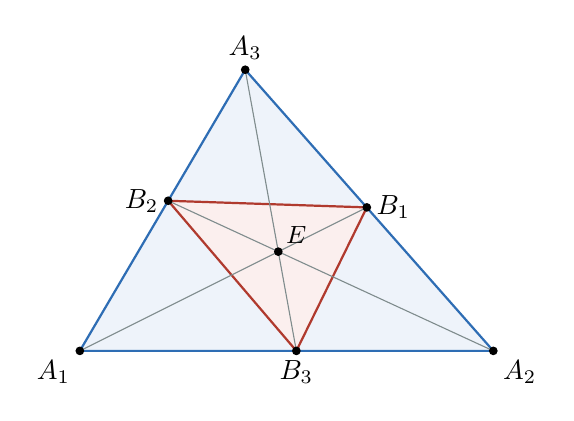
\begin{tikzpicture}[scale=1.05]
  \coordinate (A1) at (0,0); \coordinate (A2) at (5,0); \coordinate (A3) at (2,3.4); \coordinate (E) at (2.4,1.2);
  \coordinate (B1) at (intersection of A1--E and A2--A3);
  \coordinate (B2) at (intersection of A2--E and A3--A1);
  \coordinate (B3) at (intersection of A3--E and A1--A2);
  \fill[defbg] (A1)--(A2)--(A3)--cycle; \draw[defblue,thick] (A1)--(A2)--(A3)--cycle;
  \fill[thmbg] (B1)--(B2)--(B3)--cycle; \draw[thmred,thick] (B1)--(B2)--(B3)--cycle;
  \draw[figgray] (A1)--(B1) (A2)--(B2) (A3)--(B3);
  \foreach \p/\l/\pos in {A1/A_1/below left,A2/A_2/below right,A3/A_3/above,B1/B_1/right,B2/B_2/left,B3/B_3/below}{\fill (\p) circle (1.5pt) node[\pos] {$\l$};}
  \fill (E) circle (1.5pt) node[above right=-1pt] {\small $E$};
\end{tikzpicture}
\caption{$B_1=(0,1,1)\T,\ B_2=(1,0,1)\T,\ B_3=(1,1,0)\T$}
\end{figure}

\jie $A_1E:\ x_2=x_3$ 与 $A_2A_3:\ x_1=0$ 交于 $B_1=(0,1,1)\T$；同理 $B_2=(1,0,1)\T$，$B_3=(1,1,0)\T$。$\sigma(A_i)=B_i$ 意味着矩阵第 $i$ 列 $\propto\vv b_i$：
\[
\lambda\begin{pmatrix}x_1'\\x_2'\\x_3'\end{pmatrix}=\begin{pmatrix}0&\lambda_2&\lambda_3\\\lambda_1&0&\lambda_3\\\lambda_1&\lambda_2&0\end{pmatrix}\begin{pmatrix}x_1\\x_2\\x_3\end{pmatrix},\qquad \lambda_1,\lambda_2,\lambda_3\ \text{为任意非零实数}.
\]
（行列式 $=2\lambda_1\lambda_2\lambda_3\neq0$。）\key{参数计数}：只给 3 对点，$8-3\times2=2$ 个自由度——正是 $\lambda_1:\lambda_2:\lambda_3$ 的两个比值；再指定单位点的像就唯一了。

\begin{ex}{7.5.3}
在扩大的欧氏平面上，求出把直线 $x_1=0,\ x_2=0,\ x_3=0$ 分别映成直线 $a_ix_1+b_ix_2+c_ix_3=0\ (i=1,2,3)$ 的射影变换公式的一般形式。
\end{ex}
\jie 设 $\sigma:\ \lambda X'=AX$。直线 $\vv u\T X=0$ 的像是 $\vv u\T A^{-1}X'=0$，线坐标为 $(A^{-1})\T\vv u$。要求 $x_i=0$（$\vv u=\vv e_i$）的像是 $\vv l_i=(a_i,b_i,c_i)\T$：
\[
(A^{-1})\T\vv e_i=\rho_i\vv l_i\ (i=1,2,3)\ \Longleftrightarrow\ A^{-1}=\begin{pmatrix}\rho_1&0&0\\0&\rho_2&0\\0&0&\rho_3\end{pmatrix}\begin{pmatrix}a_1&b_1&c_1\\a_2&b_2&c_2\\a_3&b_3&c_3\end{pmatrix}=:DR .
\]
所以
\[
A=R^{-1}D^{-1}=\begin{pmatrix}a_1&b_1&c_1\\a_2&b_2&c_2\\a_3&b_3&c_3\end{pmatrix}^{-1}\begin{pmatrix}\rho_1^{-1}&0&0\\0&\rho_2^{-1}&0\\0&0&\rho_3^{-1}\end{pmatrix},
\]
$\rho_i$ 为任意非零实数，前提是三条像直线不共点（$|R|\neq0$）。\key{直觉}：线坐标按\key{逆转置} $(A^{-1})\T$ 变换——对偶空间的“反步变换”（高代：对偶基的过渡矩阵是 $(A\T)^{-1}$）。

\begin{ex}{7.5.4}
证明：在射影平面上，以坐标三角形的三个顶点为不动点的射影变换公式的一般形式是
\[
\lambda\begin{pmatrix}x_1'\\x_2'\\x_3'\end{pmatrix}=\begin{pmatrix}a&0&0\\0&b&0\\0&0&c\end{pmatrix}\begin{pmatrix}x_1\\x_2\\x_3\end{pmatrix},
\]
其中 $a,b,c$ 均可取任意非零实数。
\end{ex}
\zheng $A_1=(1,0,0)\T$ 不动 $\iff A\vv e_1=k_1\vv e_1\iff$ $A$ 的第一列为 $(k_1,0,0)\T$；同理第二、三列为 $(0,k_2,0)\T,(0,0,k_3)\T$。于是 $A=\operatorname{diag}(a,b,c)$，$|A|=abc\neq0$ 要求三者非零。反之这样的变换显然以 $A_1,A_2,A_3$ 为不动点。\qed\quad\gd $\vv e_1,\vv e_2,\vv e_3$ 都是特征向量 $\iff$ $A$ 是对角阵。

\begin{ex}{7.5.5}
在射影平面上，设射影变换 $\sigma$ 的公式为
$\lambda\begin{pmatrix}x_1'\\x_2'\\x_3'\end{pmatrix}=\begin{pmatrix}0&1&1\\-1&2&1\\-2&2&3\end{pmatrix}\begin{pmatrix}x_1\\x_2\\x_3\end{pmatrix}$，求 $\sigma$ 的不动点和不变直线。
\end{ex}
\jie\textbf{不动点 = $A$ 的特征向量}。$|\lambda I-A|=(\lambda-1)^2(\lambda-3)$。
\begin{itemize}
\item $\lambda=3$：$(3I-A)X=0$ 得 $X=(1,1,2)\T$；
\item $\lambda=1$：$(I-A)X=0$ 只有一个方程 $x_1-x_2-x_3=0$，解空间 2 维，基为 $(1,1,0)\T,(1,0,1)\T$。
\end{itemize}
所以不动点为 $(1,1,2)\T$ 以及 $k_1(1,1,0)\T+k_2(1,0,1)\T$（$k_1,k_2$ 不全为零）——后者就是直线 $x_1-x_2-x_3=0$ 上的\key{所有点}。

\textbf{不变直线 = $A\T$ 的特征向量}。$A\T$ 的特征值同为 $3,1,1$：
\begin{itemize}
\item $\lambda=3$：$\vv u=(1,-1,-1)\T$，直线 $x_1-x_2-x_3=0$；
\item $\lambda=1$：$(I-A\T)\vv u=\vv 0$ 的解 $\vv u=c_1(-1,1,0)\T+c_2(-2,0,1)\T$，直线 $(c_1+2c_2)x_1-c_1x_2-c_2x_3=0$（$c_1,c_2$ 不全为零）。
\end{itemize}

\begin{intbox}{看清结构：这是一个“透射”}
\begin{itemize}
\item 直线 $l_0:\ x_1-x_2-x_3=0$ \key{逐点不动}（透射轴），点 $A=(1,1,2)\T$ 不动且不在 $l_0$ 上（透射中心）；
\item 第二族不变直线 $(c_1+2c_2)x_1-c_1x_2-c_2x_3=0$ 都过 $(1,1,2)$（代入：$c_1+2c_2-c_1-2c_2=0$）——\key{过中心的直线都不变}。
\end{itemize}
对 $l_0$ 外一点 $P=\vv a+\vv p_0$（$P_0\in l_0$），$\sigma(P)=3\vv a+\vv p_0$，于是 $(A,P_0;P,P')=\frac{3}{1}=3$ 为常数——正是下一题的“透射”，特征比 $e=3$（两个特征值之比）。
\end{intbox}

\begin{ex}{7.5.6$^*$}
设射影平面上的一个点变换 $\sigma$ 有不动点 $A$ 和不动直线 $l_0$（$l_0$ 上每点均不动），$A$ 不在 $l_0$ 上，并且对于每个其他点 $P$，$\sigma$ 把 $P$ 映成 $AP$ 上的点 $P'$，使得 $(A,P_0;P,P')=e$，其中 $P_0$ 是 $AP$ 和 $l_0$ 的交点，$e$ 是常数（$\neq0,1$），证明：$\sigma$ 是射影变换。此时称 $\sigma$ 为\key{透射}，$A$ 为\key{透射中心}，$l_0$ 为\key{透射轴}。
\end{ex}

\begin{figure}[htbp]
\centering
\begin{tikzpicture}[scale=1.0]
  \draw[thick,figgreen] (-0.5,0)--(7,0) node[right] {$l_0$（逐点不动）};
  \coordinate (A) at (2.2,3.6);
  \fill[keyred] (A) circle (2pt) node[above,keyred] {$A$（中心）};
  \foreach \x/\t in {0.6/0.55,3.4/0.45,5.8/0.6}{
    \coordinate (P0) at (\x,0);
    \coordinate (P) at ($(A)!\t!(P0)$);
    \coordinate (Pp) at ($(A)!{\t/(\t+3*(1-\t))}!(P0)$);
    \draw[figgray] (A)--(P0);
    \fill (P0) circle (1.4pt);
    \fill[figblue] (P) circle (1.6pt);
    \fill[figred] (Pp) circle (1.6pt);
    \draw[->,figpur,thick,shorten >=2pt,shorten <=2pt] (P)--(Pp);}
  \node[figblue] at (3.02,1.92) {\small $P$};
  \node[figred] at (2.76,2.86) {\small $P'$};
  \node at (3.4,-0.3) {\small $P_0$};
  \node[align=left,right] at (7.1,1.8) {\small 每个点沿“射线 $AP$”移动\\\small 交比 $(A,P_0;P,P')=e$ 固定};
\end{tikzpicture}
\caption{透射：中心 $A$、轴 $l_0$、特征交比 $e$（图中 $e=3$）}
\end{figure}

\zheng 在 $l_0$ 上取两点 $A_2,A_3$，取基底 I$[A,A_2,A_3,E]$（$E$ 为一般位置点）。于是 $A=(1,0,0)\T$，$l_0:\ x_1=0$。

设 $P=(x_1,x_2,x_3)\T$ 不是 $A$ 也不在 $l_0$ 上（$x_1\neq0$）。直线 $AP$ 上的点为 $\lambda\vv a+\mu\vv p$，与 $x_1=0$ 的交点为
\[
P_0=(0,x_2,x_3)\T,\qquad\text{于是}\quad \vv p=x_1\vv a+\vv p_0 .
\]
设 $P'=\alpha\vv a+\beta\vv p_0$。由交比公式，$(A,P_0;P,P')=\dfrac{\alpha/\beta}{x_1/1}=e$，所以 $\alpha/\beta=ex_1$，取 $\beta=1$：
\[
P'=(ex_1,\ x_2,\ x_3)\T .
\]
对 $l_0$ 上的点（$x_1=0$）此式给出 $P'=P$，对 $A$ 给出 $(e,0,0)\T\sim A$，都与已知相符。所以 $\sigma$ 在基底 I 中的公式为
\[
\lambda\begin{pmatrix}x_1'\\x_2'\\x_3'\end{pmatrix}=\begin{pmatrix}e&0&0\\0&1&0\\0&0&1\end{pmatrix}\begin{pmatrix}x_1\\x_2\\x_3\end{pmatrix},
\]
系数矩阵非奇异（$e\neq0$），由定理 5.3，$\sigma$ 是射影变换。\qed

\begin{gdbox}{高代：透射的矩阵}
透射 $\iff$ 矩阵可对角化为 $\operatorname{diag}(e,1,1)$：一个单特征值（中心）+ 一个二重特征值且几何重数为 2（轴）。若二重特征值只有 1 维特征向量（不可对角化），对应的是“中心在轴上”的退化情形（称为\key{射影平移}或 elation，如 $\begin{psmallmatrix}1&1&0\\0&1&0\\0&0&1\end{psmallmatrix}$）——Jordan 标准形在几何中的样子。
\end{gdbox}

% ================= §7.6 配极，二次曲线的射影分类 =================
\Needspace{12\baselineskip}
\section{配极，二次曲线的射影分类}

\subsection{射影平面上的二次曲线}

\begin{defbox}{二次曲线}
射影坐标满足二次齐次方程
\begin{equation}
a_{11}x_1^2+a_{22}x_2^2+a_{33}x_3^2+2a_{12}x_1x_2+2a_{13}x_1x_3+2a_{23}x_2x_3=0
\quad\Longleftrightarrow\quad X\T AX=0\ \ (A\T=A)
\end{equation}
的点的集合称为\key{二次曲线} $\Sb$。$|A|\neq0$ 称为\key{非退化}的，否则为\key{退化}的。换基底时 $A\mapsto H\T AH$（合同），方程仍是二次齐次的。
\end{defbox}

\begin{gdbox}{与第五章记号对照}
第五章 $F(x,y)=a_{11}x^2+2a_{12}xy+a_{22}y^2+2a_1x+2a_2y+a_0$，矩阵 $P=\begin{psmallmatrix}a_{11}&a_{12}&a_1\\a_{12}&a_{22}&a_2\\a_1&a_2&a_0\end{psmallmatrix}$。齐次化（$x=\frac{x_1}{x_3},y=\frac{x_2}{x_3}$，乘 $x_3^2$）就是本章的 $A$：$a_{13}=a_1,\ a_{23}=a_2,\ a_{33}=a_0$，$|A|=I_3$。第五章“$I_3\neq0$”的曲线就是这里的非退化二次曲线。
\end{gdbox}

在直角坐标系的齐次坐标下：
\begin{itemize}
\item \textbf{情形 1}（$a_{11},a_{12},a_{22}$ 不全为零）：通常点满足原来的 $F(x,y)=0$；无穷远点 $(x_1,x_2,0)\T$ 在 $\Sb$ 上 $\iff a_{11}x_1^2+2a_{12}x_1x_2+a_{22}x_2^2=0$，即 $(x_1,x_2)$ 是\key{渐近方向}。所以 $\Sb$ = 欧氏二次曲线 + 它的渐近方向对应的无穷远点。
\item \textbf{情形 2}（$a_{11}=a_{12}=a_{22}=0$）：$x_3(2a_{13}x_1+2a_{23}x_2+a_{33}x_3)=0$——一条射影直线和无穷远直线，或一对重合的无穷远直线。
\end{itemize}
所以 $\pib$ 上的二次曲线共 \key{11 种}：第五章的 9 种（补上渐近方向的无穷远点）+ 上面 2 种。

\begin{figure}[htbp]
\centering
\begin{tikzpicture}[scale=0.85]
  \foreach \sh/\d/\name/\n/\col in {0/1.75/椭圆/0 个实交点/figblue, 5/1.2/抛物线/1 个交点（相切）/figgreen, 10/0.55/双曲线/2 个交点/figred}{
    \begin{scope}[xshift=\sh cm]
      \fill[\col!10] (0,0) circle (1.2); \draw[\col,thick] (0,0) circle (1.2);
      \draw[figor,very thick] (-1.9,\d)--(1.9,\d) node[right,figor] {\small $l_\infty$};
      \node at (0,-1.65) {\small\textbf{\name}};
      \node at (0,-2.15) {\small 与 $l_\infty$：\n};
    \end{scope}}
  \fill[figgreen] (5,1.2) circle (1.8pt);
  \fill[figred] ({10-0.99},0.55) circle (1.8pt) ({10+0.99},0.55) circle (1.8pt);
\end{tikzpicture}
\caption{射影眼中三种圆锥曲线是\key{同一条}非退化二次曲线（画成圆），区别只在无穷远直线的位置：椭圆与 $l_\infty$ 不交，抛物线与 $l_\infty$ 相切，双曲线与 $l_\infty$ 交于两点（两个渐近方向）}
\end{figure}

\begin{mtbox}{例：用无穷远点判断类型}
$x^2-3xy+2y^2+x-1=0$：令 $x_3=0$，$x_1^2-3x_1x_2+2x_2^2=(x_1-x_2)(x_1-2x_2)=0$，两个实无穷远点 $(1,1,0)\T,(2,1,0)\T$，且 $|A|=-\frac14\neq0$，所以是\key{双曲线}，渐近方向 $(1,1)$ 与 $(2,1)$。\\
$x^2+2xy+y^2+x=0$：$(x_1+x_2)^2=0$，一个二重无穷远点 $(1,-1,0)\T$，$|A|=-\frac14\neq0$，\key{抛物线}（与 $l_\infty$ 相切）。
\end{mtbox}

\subsection{二次曲线的切线}
把直线 $PQ$ 的参数方程 $\vv x=\lambda\vv p+\mu\vv q$ 代入 $X\T AX=0$：
\begin{equation}
\lambda^2F(\vv p)+2\lambda\mu\,\overline F(\vv p;\vv q)+\mu^2F(\vv q)=0,\qquad \overline F(\vv p;\vv q):=\vv p\T A\vv q .
\end{equation}
三个系数全为零时整条直线在 $\Sb$ 上；否则它确定 $\lambda:\mu$ 的两个值（相异、重合或虚），即直线与 $\Sb$ 有两个交点。

\begin{defbox}{定义 6.1（切线）、奇点}
直线 $L$ 与 $\Sb$ 有\key{重合的两个交点}或 $L$ 整个在 $\Sb$ 上，称 $L$ 为\key{切线}，交点为切点。\\
设切点 $P\in\Sb$。由判别式 $\overline F(\vv p;\vv q)^2-F(\vv p)F(\vv q)=0$ 及 $F(\vv p)=0$ 得 $\overline F(\vv p;\vv q)=0$，所以切线方程为
\begin{equation}
\vv p\T AX=0 .
\end{equation}
若 $\vv p\T A=\vv0$，过 $P$ 的每条直线都是切线，$P$ 称为\key{奇点}。非退化二次曲线没有奇点。
\end{defbox}

\begin{thmbox}{二级结论：“半代换”写切线}
$\vv p\T AX=0$ 展开就是第五章的切线公式：$x^2\to x_0x$，$xy\to\frac{x_0y+xy_0}{2}$，$x\to\frac{x+x_0}{2}$，$y\to\frac{y+y_0}2$，常数不变。例如椭圆 $\frac{x^2}{a^2}+\frac{y^2}{b^2}=1$ 在 $(x_0,y_0)$ 处切线 $\frac{x_0x}{a^2}+\frac{y_0y}{b^2}=1$；抛物线 $y^2=2px$：$y_0y=p(x+x_0)$。
\end{thmbox}

\subsection{极点和极线}

\begin{defbox}{极线（用调和共轭定义）}
$P\notin\Sb$。过 $P$ 任作直线交 $\Sb$ 于 $G,H$，作 $P$ 关于 $G,H$ 的调和共轭点 $Q$：$(G,H;P,Q)=-1$。$Q$ 的轨迹称为 $P$ 关于 $\Sb$ 的\key{配极}（\key{极线}），$P$ 叫\key{极点}。其方程为
\begin{equation}
\vv p\T AX=0\qquad\Big(\text{即}\ \sum_{i,j}a_{ij}p_ix_j=0\Big).
\end{equation}
$P\in\Sb$ 时，把在 $P$ 的切线也叫 $P$ 的极线（方程同形）。
\end{defbox}

\noindent\textbf{推导}：$G,H$ 对应 (6.6) 的两根 $\frac{\lambda_1}{\mu_1},\frac{\lambda_2}{\mu_2}$，$(P,Q;G,H)=\frac{\lambda_2/\mu_2}{\lambda_1/\mu_1}=-1$ 即 $\frac{\lambda_1}{\mu_1}+\frac{\lambda_2}{\mu_2}=0$——两根之和为零，由 Vieta，一次项系数 $2\overline F(\vv p;\vv q)=0$。\qed

\begin{figure}[htbp]
\centering
\begin{tikzpicture}[scale=1.25]
  \fill[defbg] (0,0) ellipse (2 and 1); \draw[thick,defblue] (0,0) ellipse (2 and 1);
  \coordinate (P) at (4,0); \coordinate (T1) at (1,0.866); \coordinate (T2) at (1,-0.866);
  \draw[figgreen,thick] ($(P)!-0.1!(T1)$)--($(P)!1.35!(T1)$); \draw[figgreen,thick] ($(P)!-0.1!(T2)$)--($(P)!1.35!(T2)$);
  \draw[figred,very thick] (1,-1.45)--(1,1.45) node[above,figred] {\small 极线 $x=1$};
  \coordinate (G) at (1.843,0.388); \coordinate (H) at (-0.925,0.886); \coordinate (Q) at (1,0.54);
  \draw[figpur] (P)--($(P)!1.08!(H)$);
  \fill (P) circle (1.7pt) node[right] {$P(4,0)$};
  \foreach \p/\pos in {T1/above left,T2/below left}{\fill[figgreen] (\p) circle (1.6pt);}
  \node[figgreen,above left] at (T1) {\small $T_1$}; \node[figgreen,below left] at (T2) {\small $T_2$};
  \fill[figpur] (G) circle (1.5pt) node[above right=-1pt,figpur] {\small $G$};
  \fill[figpur] (H) circle (1.5pt) node[above left,figpur] {\small $H$};
  \fill[keyred] (Q) circle (1.6pt) node[above left=-1pt,keyred] {\small $Q$};
  \node at (-1.2,-0.3) {\small $\frac{x^2}{4}+y^2=1$};
\end{tikzpicture}
\caption{$P(4,0)$ 关于椭圆 $\frac{x^2}4+y^2=1$ 的极线 $x=1$：它是切点弦 $T_1T_2$，也是每条割线上 $P$ 的调和共轭点 $Q$ 的轨迹，$(G,H;P,Q)=-1$}
\end{figure}

\begin{mtbox}{例：椭圆 $\frac{x^2}{4}+y^2=1$，$P(4,0)$}
$A=\operatorname{diag}(\frac14,1,-1)$，$\vv p\T A=(4,0,1)\,A=(1,0,-1)$，极线 $x_1-x_3=0$，即 $x=1$。它交椭圆于 $T_{1,2}=(1,\pm\frac{\sqrt3}2)$，在 $T_1$ 的切线 $\frac{x}{4}+\frac{\sqrt3}{2}y=1$ 确实过 $(4,0)$。随便一条割线 $y=-0.18(x-4)$ 交椭圆于 $G(1.843,0.388),H(-0.925,0.886)$，交极线于 $Q(1,0.54)$，用横坐标验算：$(G,H;P,Q)=\frac{(4-1.843)(1+0.925)}{(4+0.925)(1-1.843)}=-1$。\checkmark
\end{mtbox}

\begin{thmbox}{极线的两条基本性质（配极原理）}
(1) \key{对称性}：$Q$ 在 $P$ 的极线上 $\iff$ $P$ 在 $Q$ 的极线上。（因为 $\vv p\T A\vv q=\vv q\T A\vv p$，$A$ 对称。此时称 $P,Q$ \key{共轭}。）\\
(2) $P$ 的极线过 $P$ $\iff$ $P\in\Sb$。\\[2pt]
\textbf{推论（切点弦）}：$P$ 在 $\Sb$ 外时，从 $P$ 引的两条切线的切点 $T_1,T_2$ 都在 $P$ 的极线上（$T_i$ 的切线过 $P$ $\Rightarrow$ $P$ 在 $T_i$ 的极线上 $\Rightarrow$ $T_i$ 在 $P$ 的极线上），所以极线就是\key{切点弦}。
\end{thmbox}

\begin{defbox}{定义 6.2（配极映射）}
$\Sb$ 非退化时，每点 $P$ 有唯一极线 $L_P$（线坐标 $A\vv p$）；每条直线 $\vv b\T X=0$ 有唯一极点 $\vv p=A^{-1}\vv b$。对应 $P\leftrightarrow L_P$ 称为关于 $\Sb$ 的\key{配极映射}，它把点变成线、线变成点，\key{保持关联}（由性质 (1)）——对偶原理的一个“具体实现”。
\end{defbox}

\begin{gdbox}{高代联动：配极 = 非退化对称双线性型}
$\langle\vv p,\vv q\rangle_A:=\vv p\T A\vv q$ 是 $\R^3$ 上的对称双线性型。极线 = “$A$-正交补” $\vv p^{\perp_A}$；共轭点 = $A$-正交向量；二次曲线上的点 = \key{迷向向量}（$\langle\vv p,\vv p\rangle_A=0$）。$A$ 非退化 $\iff$ $\vv p\mapsto\langle\vv p,\cdot\rangle_A$ 是同构 $V\to V^*$——这就是“点 $\leftrightarrow$ 线”的配极映射。
\end{gdbox}

\begin{thmbox}{用配极统一第五章的概念（证明见习题 7.6）}
\renewcommand{\arraystretch}{1.25}
\begin{tabularx}{\linewidth}{@{}>{\raggedright\arraybackslash}p{0.33\linewidth}>{\raggedright\arraybackslash}X@{}}
\toprule
第五章的概念 & 射影的说法\\\midrule
切线 & 曲线上的点的极线\\
中心 & \key{无穷远直线的极点}（第 5 题）\\
共轭于方向 $\vv v$ 的直径 & \key{无穷远点 $\vv v$ 的极线}（第 4 题）\\
渐近线 & 曲线上无穷远点处的切线（第 6 题）\\
抛物线没有中心 & \key{无穷远直线与抛物线相切}，极点在 $l_\infty$ 上（第 7 题）\\
准线 & \key{焦点的极线}（第 8 题）\\
两直径互相共轭 & 两个无穷远点关于 $\Sb$ 共轭\\\bottomrule
\end{tabularx}
\end{thmbox}

\subsection{自配极三角形}

\begin{defbox}{定义 6.3、定理 6.1}
$\triangle ABC$ 的每条边是对顶点的极线，称为关于 $\Sb$ 的\key{自配极三角形}。\key{任一二次曲线都存在自配极三角形}。\\[2pt]
\textbf{构造}：在 $\Sb$ 外取 $A$，作极线 $L_A$（$A\notin L_A$）；在 $L_A$ 上取不在 $\Sb$ 上的 $B$，作极线 $L_B$（$B\in L_A\Rightarrow A\in L_B$）；令 $C=L_A\cap L_B$。则 $C$ 在 $L_A,L_B$ 上 $\Rightarrow$ $A,B$ 都在 $C$ 的极线上 $\Rightarrow$ $L_C=AB$。（$L_A$ 整个在 $\Sb$ 上时，$\Sb$ 是一对重合直线，$L_A$ 上任取两点即可。）
\end{defbox}

\begin{figure}[htbp]
\centering
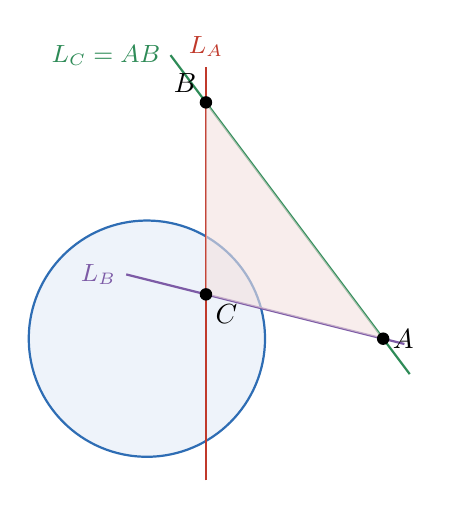
\begin{tikzpicture}[scale=1.5]
  \fill[defbg] (0,0) circle (1); \draw[thick,defblue] (0,0) circle (1);
  \coordinate (A) at (2,0); \coordinate (B) at (0.5,2); \coordinate (C) at (0.5,0.375);
  \draw[figred,thick] (0.5,-1.2)--(0.5,2.3) node[above,figred] {\small $L_A$};
  \draw[figgreen,thick] ($(A)!-0.15!(B)$)--($(A)!1.2!(B)$) node[left,figgreen] {\small $L_C=AB$};
  \draw[figpur,thick] ($(A)!-0.12!(C)$)--($(A)!1.45!(C)$) node[left,figpur] {\small $L_B$};
  \fill[thmred!15,opacity=0.6] (A)--(B)--(C)--cycle;
  \foreach \p/\pos in {A/right,B/above left,C/below right}{\fill (\p) circle (1.5pt) node[\pos] {$\p$};}
\end{tikzpicture}
\caption{单位圆的自配极三角形：$A(2,0)$ 的极线 $x=\frac12$，$B(\frac12,2)$ 的极线 $\frac x2+2y=1$，$C=(\frac12,\frac38)$；$C$ 的极线 $\frac x2+\frac{3y}8=1$ 恰是 $AB$}
\end{figure}

\begin{gdbox}{高代联动：自配极三角形 = 合同对角化}
以自配极三角形 $ABC$ 为坐标三角形，“$BC$ 是 $A$ 的极线”给出 $a_{12}^*=a_{13}^*=0$，同理 $a_{23}^*=0$：方程变为 $a_{11}^*x_1^2+a_{22}^*x_2^2+a_{33}^*x_3^2=0$。三顶点 = 三个两两 $A$-正交的向量，以它们为列的矩阵 $C$ 使 $C\T AC$ 对角——这就是\key{二次型的合同对角化}的几何图像。
\end{gdbox}

\subsection{二次曲线的射影分类}
对角化后再作 $\rho x_i^*=\tilde x_i/\sqrt{|\lambda_i|}$，并适当排列顶点、整体乘 $-1$，得到：

\begin{thmbox}{定理 6.2（射影分类：5 类）}
射影平面上的二次曲线分成五个射影类，代表为
\begin{equation}
x_1^2+x_2^2+x_3^2=0,\quad x_1^2+x_2^2-x_3^2=0,\quad x_1^2+x_2^2=0,\quad x_1^2-x_2^2=0,\quad x_1^2=0 .
\end{equation}
前两类非退化，后三类退化。分类依据：$A$ 的\key{秩}和\key{符号差的绝对值}（$A$ 与 $-A$ 是同一条曲线）。
\end{thmbox}

\begin{center}
\renewcommand{\arraystretch}{1.3}
\begin{tabularx}{\linewidth}{@{}>{\centering\arraybackslash}p{3.2cm}>{\centering\arraybackslash}p{2.6cm}>{\raggedright\arraybackslash}X@{}}
\toprule
射影类代表 & 秩，$|$符号差$|$ & $\pib$ 上的 11 种二次曲线中属于此类的\\\midrule
$x_1^2+x_2^2+x_3^2=0$ & 3，\ 3 & 虚椭圆（无轨迹）\\
$x_1^2+x_2^2-x_3^2=0$ & 3，\ 1 & \key{椭圆、双曲线、抛物线}\\
$x_1^2+x_2^2=0$ & 2，\ 2 & 一对虚相交直线（只有一个实点）、一对虚平行直线\\
$x_1^2-x_2^2=0$ & 2，\ 0 & 一对相交直线、一对平行直线、一条射影直线 + $l_\infty$\\
$x_1^2=0$ & 1，\ 1 & 一对重合直线、一对重合的无穷远直线\\\bottomrule
\end{tabularx}
\end{center}

\begin{gdbox}{高代联动：惯性定理}
实对称矩阵在合同变换下的全系不变量是\key{秩}与\key{正惯性指数}（等价地，秩与符号差）。射影类再把 $A$ 与 $-A$ 视为同一（方程两边乘 $-1$），所以只看 $|$符号差$|$：秩 3 有 $|s|=3,1$；秩 2 有 $|s|=2,0$；秩 1 有 $|s|=1$——共 5 类。对比：仿射分类（第六章）9 类，因为仿射变换必须保持 $l_\infty$，多了“与 $l_\infty$ 的位置关系”这个不变量。
\end{gdbox}

\begin{figure}[htbp]
\centering
\begin{tikzpicture}[scale=0.95]
  \coordinate (V) at (0,0);
  \draw[thick] (-2.2,2.6)--(2.2,-2.6); \draw[thick] (2.2,2.6)--(-2.2,-2.6);
  \draw[thick] (0,2.6) ellipse (2.2 and 0.35); \draw[thick,dashed] (0,-2.6) ellipse (2.2 and 0.35);
  \draw[figblue,very thick] (-1.387,1.637)--(1.919,2.265) node[right,figblue] {\small 椭圆};
  \draw[figgreen,very thick] (0.424,0.5)--(-1.356,2.6) node[above left,figgreen] {\small 抛物线（平行于母线）};
  \draw[figred,very thick] (0.75,-2.4)--(1.25,2.4) node[above right,figred] {\small 双曲线（截两叶）};
  \fill (V) circle (1.6pt) node[left] {\small 顶点 $O$};
  \node[align=left,right] at (2.9,-0.6) {\small 以 $O$ 为中心的中心投影\\\small 把一种截线变成另一种：\\\small 三者射影等价};
\end{tikzpicture}
\caption{圆锥截线（侧视示意）：同一圆锥面被不同平面所截，得到椭圆、抛物线、双曲线}
\end{figure}

\subsection{Steiner 定理，Pascal 定理，Brianchon 定理$^*$}
（本节的非退化二次曲线都指有实轨迹的。）

\begin{thmbox}{Steiner（斯坦纳）定理}
非退化二次曲线 $\Sb$ 上给定四个不同的点 $A_1,A_2,A_3,A_4$，则 $\Sb$ 上任一点 $P$ 与它们的连线的交比 $(PA_1,PA_2;PA_3,PA_4)$ 是常数；$P$ 与某个 $A_i$（如 $A_4$）重合时，用该点的切线 $A_4T$ 代替 $PA_4$，交比仍等于这个常数。
\end{thmbox}
\noindent\textbf{证明要点}：$A_1,\dots,A_4$ 一般位置，取基底 $[A_1,A_2,A_3,A_4]$。$\Sb$ 过 $A_1,A_2,A_3$ 得 $a_{11}=a_{22}=a_{33}=0$，过 $A_4=(1,1,1)$ 得 $a_{12}+a_{13}+a_{23}=0$，可设方程为 $x_2x_3-kx_1x_3+(k-1)x_1x_2=0$（$k\neq0,1$）。对 $\Sb$ 上的 $P(x_1,x_2,x_3)$，直接算出 $(PA_1,PA_2;PA_3,PA_4)=\frac{x_2(x_1-x_3)}{x_1(x_2-x_3)}$，由方程它恒等于 $k$。$P\to A_4$ 时割线 $PA_4\to$ 切线，取极限即得后半部分。（圆的情形就是习题 7.3 第 10 题。）

\begin{thmbox}{Pascal（巴斯卡）定理}
非退化二次曲线的\key{内接六角形的三对对边的交点共线}：若 $A,B,C,A',B',C'$ 在 $\Sb$ 上，$AB'\cap A'B=P$，$AC'\cap A'C=Q$，$BC'\cap B'C=R$，则 $P,Q,R$ 共线（\key{Pascal 线}）。\\[2pt]
\textbf{Brianchon（布里昂香）定理}（Pascal 的对偶）：非退化二次曲线的\key{外切六边形的三对对顶点连线共点}。
\end{thmbox}

\begin{figure}[htbp]
\centering
\begin{tikzpicture}[scale=1.25]
  \draw[thick,defblue] (0,0) ellipse (2.6 and 1.5);
  \coordinate (A) at (-1.992,0.964); \coordinate (B) at (1.099,1.359); \coordinate (C) at (2.511,0.388);
  \coordinate (A') at (-2.511,-0.388); \coordinate (B') at (-0.889,-1.410); \coordinate (C') at (1.671,-1.149);
  \coordinate (P) at (intersection of A--B' and A'--B);
  \coordinate (Q) at (intersection of A--C' and A'--C);
  \coordinate (R) at (intersection of B--C' and B'--C);
  \draw[figblue!70] (A)--(B') (A')--(B);
  \draw[figgreen!80!black] (A)--(C') (A')--(C);
  \draw[figred!80] (B)--(C') (B')--(C);
  \draw[keyred,very thick] ($(P)!-0.35!(R)$)--($(P)!1.3!(R)$) node[right,keyred] {\small Pascal 线};
  \foreach \p/\pos in {A/above left,B/above,C/right,A'/left,B'/below,C'/below right}{\fill (\p) circle (1.6pt) node[\pos] {$\p$};}
  \foreach \p/\pos in {P/above left,Q/below,R/above}{\fill[keyred] (\p) circle (1.8pt) node[\pos,keyred] {\small $\p$};}
\end{tikzpicture}
\caption{Pascal 定理：内接六角形 $AB'CA'BC'$ 的三对对边交点 $P,Q,R$ 共线}
\end{figure}

\noindent\textbf{Pascal 定理的证明要点}：设 $BC'$ 交 $PQ$ 于 $R_1$，要证 $R_1=R$。记 $H=BC'\cap A'C$，$G=AC'\cap A'B$。四次换“视点”：
\begin{align*}
(B,H;C',R_1)&\overset{Q}{=}(B,A';G,P)\overset{A}{=}(AB,AA';AC',AB')\\
&\overset{\text{Steiner}}{=}(CB,CA';CC',CB')\overset{C}{=}(B,H;C',R),
\end{align*}
于是 $R_1=R$。\qed

\begin{intbox}{直觉：Pascal 退化 = Pappus}
把二次曲线退化成两条直线 $l_1\cup l_2$（$A,B,C\in l_1$，$A',B',C'\in l_2$），Pascal 定理就变成习题 7.4 第 5 题的 Pappus 定理。Pascal 还给出了“五点作二次曲线”的直尺作图法：已知五点，任作过其中一点的直线，用 Pascal 线就能作出它与曲线的第二个交点。
\end{intbox}

\begin{thmbox}{二级结论：完备四点形的调和性（习题 7.6 第 9、12 题要用）}
完备四点形 $ABCD$ 的一边（如 $AC$）上：两个顶点 $A,C$ 被该边上的对角点 $F=AC\cap BD$ 和该边与另两个对角点连线的交点 $F_1=AC\cap GH$ \key{调和分割}：$(A,C;F,F_1)=-1$。\\[2pt]
\textbf{证明}：基底 $[A,B,C,D]$，$F=(1,0,1)\T=\vv a+\vv c$，$G=AD\cap BC=(0,1,1)\T$，$H=AB\cap CD=(1,1,0)\T$，$GH:\ -x_1+x_2-x_3=0$，$F_1=GH\cap AC=(1,0,-1)\T=\vv a-\vv c$，故交比为 $-1$。\qed
\end{thmbox}

% ---------------- 习题 7.6 ----------------
\xiti{7.6}

\begin{ex}{7.6.1}
在射影平面上给了下列五个点，求由它们所确定的二次曲线：$A(1,-1,0)\T$，$B(2,0,-1)\T$，$C(0,2,-1)\T$，$D(1,4,-2)\T$，$E(2,3,-2)\T$。
\end{ex}
\jie 设 $\Sb:\ a_{11}x_1^2+a_{22}x_2^2+a_{33}x_3^2+2a_{12}x_1x_2+2a_{13}x_1x_3+2a_{23}x_2x_3=0$，代入五点得 5 个关于 6 个系数的齐次线性方程：
\begin{align*}
A:&\ a_{11}+a_{22}-2a_{12}=0, \qquad B:\ 4a_{11}+a_{33}-4a_{13}=0, \qquad C:\ 4a_{22}+a_{33}-4a_{23}=0,\\
D:&\ a_{11}+16a_{22}+4a_{33}+8a_{12}-4a_{13}-16a_{23}=0,\\
E:&\ 4a_{11}+9a_{22}+4a_{33}+12a_{12}-8a_{13}-12a_{23}=0 .
\end{align*}
系数矩阵秩为 5，解空间 1 维：$a_{11}=a_{22}=a_{12}=\frac49a_{23},\ a_{33}=\frac{20}9a_{23},\ a_{13}=a_{23}$。取 $a_{23}=\frac92$：
\[
2x_1^2+2x_2^2+10x_3^2+4x_1x_2+9x_1x_3+9x_2x_3=0 .
\]

\begin{intbox}{看清本质：它是两条直线}
左边可分解：$2x_1^2+\dots=(x_1+x_2+2x_3)(2x_1+2x_2+5x_3)$。验证：$A,B,C$ 都满足 $x_1+x_2+2x_3=0$——\key{三点共线}！$D,E$ 满足 $2x_1+2x_2+5x_3=0$。\\
原因：二次曲线与一条直线最多两个交点，除非整条直线在曲线上（\S7.6.2）。所以过 $A,B,C$ 的二次曲线必须包含直线 $ABC$，剩下部分是一条过 $D,E$ 的直线——答案唯一而且退化。这说明第 13 题“\key{一般位置}五点”的条件不能去掉。
\end{intbox}

\begin{ex}{7.6.2}
求经过点 $A(1,0,1)\T$，$B(0,1,1)\T$，$C(0,-1,1)\T$ 且以直线 $l_1:\ x_1-x_3=0$ 和直线 $l_2:\ x_3-x_2=0$ 为切线的二次曲线。
\end{ex}
\jie $A\in l_1$，所以 $l_1$ 是以 $A$ 为切点的切线；$B\in l_2$，$l_2$ 是以 $B$ 为切点的切线。由切线方程 $\vv p\T AX=0$：
\begin{itemize}
\item 过 $A,B,C$：$a_{11}+2a_{13}+a_{33}=0$，$a_{22}+2a_{23}+a_{33}=0$，$a_{22}-2a_{23}+a_{33}=0$ $\Rightarrow a_{23}=0,\ a_{22}=-a_{33}$；
\item 在 $A$ 的切线 $(1,0,1)A=(a_{11}+a_{13},\ a_{12}+a_{23},\ a_{13}+a_{33})\propto(1,0,-1)$ $\Rightarrow a_{12}=0$；
\item 在 $B$ 的切线 $(0,1,1)A=(a_{12}+a_{13},\ a_{22}+a_{23},\ a_{23}+a_{33})\propto(0,-1,1)$ $\Rightarrow a_{13}=0$。
\end{itemize}
再由第一式 $a_{11}=-a_{33}$。取 $a_{33}=-1$：
\[
x_1^2+x_2^2-x_3^2=0 .
\]
\begin{figure}[htbp]
\centering
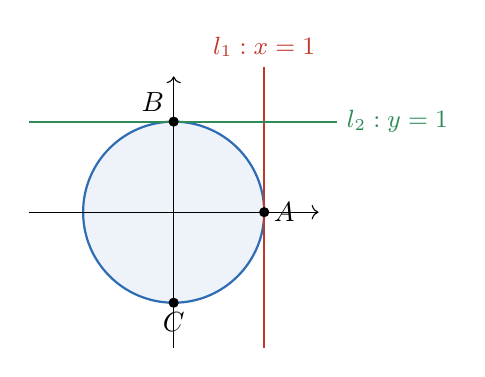
\begin{tikzpicture}[scale=1.15]
  \fill[defbg] (0,0) circle (1); \draw[thick,defblue] (0,0) circle (1);
  \draw[figred,thick] (1,-1.5)--(1,1.6) node[above,figred] {\small $l_1:x=1$};
  \draw[figgreen,thick] (-1.6,1)--(1.8,1) node[right,figgreen] {\small $l_2:y=1$};
  \foreach \p/\l/\pos in {{(1,0)}/A/right,{(0,1)}/B/above left,{(0,-1)}/C/below}{\fill \p circle (1.6pt) node[\pos] {$\l$};}
  \draw[->] (-1.6,0)--(1.6,0); \draw[->] (0,-1.5)--(0,1.5);
\end{tikzpicture}
\caption{就是单位圆 $x^2+y^2=1$}
\end{figure}

\noindent\textbf{仿射验算}：单位圆 $x^2+y^2=1$ 过 $(1,0),(0,1),(0,-1)$，在 $(1,0)$ 的切线是 $x=1$，在 $(0,1)$ 的切线是 $y=1$。\checkmark\quad 条件计数：3 个点 + 2 条切线（每条“已知切点的切线”比单纯过该点多 1 个条件）$=5$ 个线性条件，恰好定出一条二次曲线。

\begin{ex}{7.6.3}
求点 $P(1,2,1)\T$ 关于二次曲线 $\Sb:\ x_1^2-x_2^2+x_3^2-2x_1x_2-4x_1x_3=0$ 的极线。
\end{ex}
\jie $A=\begin{pmatrix}1&-1&-2\\-1&-1&0\\-2&0&1\end{pmatrix}$，$\vv p\T A=(1,2,1)A=(1-2-2,\ -1-2+0,\ -2+0+1)=(-3,-3,-1)$。极线：
\[
3x_1+3x_2+x_3=0 .
\]
（$F(\vv p)=1-4+1-4-4=-10\neq0$，$P$ 不在 $\Sb$ 上，极线不过 $P$：$3+6+1\neq0$。）

\begin{ex}{7.6.4}
证明：不在二次曲线 $\Sb$ 上的每个无穷远点的极线是共轭于此无穷远点所对应的方向的直径。
\end{ex}
\zheng\textbf{代数}：无穷远点 $\infty_1=(\mu,\nu,0)\T$，极线
\[
(\mu,\nu,0)AX=\mu(a_{11}x_1+a_{12}x_2+a_{13}x_3)+\nu(a_{12}x_1+a_{22}x_2+a_{23}x_3)=0,
\]
回到仿射坐标即 $\mu F_1(x,y)+\nu F_2(x,y)=0$，正是第五章\key{共轭于方向 $(\mu,\nu)$ 的直径}的方程（$\infty_1\notin\Sb$ 说明 $(\mu,\nu)$ 不是渐近方向）。

\textbf{几何}：以 $(\mu,\nu)$ 为方向的弦 $AB$ 上，$\infty_1$ 关于 $A,B$ 的调和共轭点是\key{弦的中点}（中点 $\leftrightarrow$ 无穷远点）。所以 $\infty_1$ 的极线 = 这组平行弦中点的轨迹 = 共轭于该方向的直径。\qed

\begin{ex}{7.6.5}
证明：非退化二次曲线 $\Sb$ 的中心（若有的话）的极线是无穷远直线。
\end{ex}
\zheng 中心 $O(x_0,y_0)$ 满足 $F_1(x_0,y_0)=F_2(x_0,y_0)=0$（第五章）。其极线
\[
(x_0,y_0,1)AX=F_1(x_0,y_0)x_1+F_2(x_0,y_0)x_2+F_3(x_0,y_0)x_3=F_3(x_0,y_0)\,x_3=0,
\]
其中 $F_3=a_{13}x+a_{23}y+a_{33}$。若 $F_3(x_0,y_0)=0$，则 $(x_0,y_0,1)A=\vv0$，与 $A$ 非奇异矛盾。所以极线是 $x_3=0$，即无穷远直线。

\textbf{几何}：过中心的弦被中心平分，中心关于弦两端的调和共轭点是无穷远点，所以中心的极线由无穷远点组成。\qed\quad（等价说法：\key{中心 = 无穷远直线的极点}，方程 $A\vv c\propto(0,0,1)\T$ 正是第五章的中心方程组 $A_0\vv\alpha_0=-\vv\delta$。）

\begin{ex}{7.6.6}
证明：双曲线上的无穷远点的极线是它的渐近线，从而双曲线上无穷远点处的切线是渐近线。
\end{ex}
\zheng 设 $\infty$ 是双曲线上的无穷远点（渐近方向）。
\begin{itemize}
\item 由第 5 题，中心 $O$ 的极线是 $l_\infty$，而 $\infty\in l_\infty$，由配极原理，$O$ 在 $\infty$ 的极线上；
\item $\infty$ 在双曲线上，所以它的极线经过它自身（性质 (2)）。
\end{itemize}
于是 $\infty$ 的极线是过中心、沿渐近方向的直线——\key{渐近线}。又曲线上点的极线就是该点处的切线，故渐近线是双曲线在无穷远点处的切线。\qed

\begin{intbox}{直觉}
“渐近线是在无穷远处与曲线相切的直线”——这句话在欧氏平面里只是比喻，在射影平面里是字面意思。
\end{intbox}

\begin{ex}{7.6.7}
证明：抛物线上的无穷远点的极线是无穷远直线，从而无穷远直线是抛物线的切线。
\end{ex}
\zheng 设抛物线上的无穷远点为 $\infty_0$（唯一的渐近方向）。$\infty_0$ 在曲线上，其极线过 $\infty_0$。再证这条极线还过另一个无穷远点：任取不在抛物线上的无穷远点 $\infty$，由第 4 题，$\infty$ 的极线是共轭于它的直径，而\key{抛物线的每条直径都沿渐近方向}（第五章），即都过 $\infty_0$；由配极原理，$\infty$ 在 $\infty_0$ 的极线上。所以 $\infty_0$ 的极线含两个不同的无穷远点，就是 $l_\infty$。于是 $l_\infty$ 是抛物线在 $\infty_0$ 处的切线。\qed

\textbf{代数验证}：$y^2=2px$，$A=\begin{psmallmatrix}0&0&-p\\0&1&0\\-p&0&0\end{psmallmatrix}$，$\infty_0=(1,0,0)\T$，$(1,0,0)A=(0,0,-p)$，极线 $x_3=0$。\checkmark

\begin{ex}{7.6.8}
证明：圆锥曲线（即椭圆、双曲线和抛物线）的焦点的极线是准线。
\end{ex}
\zheng 取标准方程逐一计算（用“半代换”）：
\begin{itemize}
\item 椭圆 $\frac{x^2}{a^2}+\frac{y^2}{b^2}=1$，焦点 $(c,0)$：极线 $\frac{cx}{a^2}=1$，即 $x=\frac{a^2}c$——准线；
\item 双曲线 $\frac{x^2}{a^2}-\frac{y^2}{b^2}=1$，焦点 $(c,0)$：极线 $\frac{cx}{a^2}=1$，即 $x=\frac{a^2}c$——准线；
\item 抛物线 $y^2=2px$，焦点 $(\frac p2,0)$：极线 $0\cdot y=p\left(x+\frac p2\right)$，即 $x=-\frac p2$——准线。
\end{itemize}
另一焦点由对称性同理。\qed

\begin{figure}[htbp]
\centering
\begin{tikzpicture}[scale=1.3]
  \fill[defbg] (0,0) ellipse (2 and 1.2); \draw[thick,defblue] (0,0) ellipse (2 and 1.2);
  \coordinate (F) at (1.6,0); \coordinate (M1) at (1.886,0.400); \coordinate (M2) at (0.818,-1.095); \coordinate (T) at (2.5,-0.643);
  \draw[figred,very thick] (2.5,-1.5)--(2.5,1.5) node[above,figred] {\small 准线 $x=\frac{a^2}{c}$};
  \draw[figpur,thick] ($(M2)!-0.1!(M1)$)--($(M2)!1.15!(M1)$);
  \draw[figgreen,thick] ($(M1)!-0.4!(T)$)--($(M1)!1.25!(T)$);
  \draw[figgreen,thick] ($(M2)!-0.2!(T)$)--($(M2)!1.15!(T)$);
  \fill (F) circle (1.6pt) node[below left=-1pt] {\small $F$};
  \fill[figpur] (M1) circle (1.5pt) node[above left=-1pt,figpur] {\small $M_1$};
  \fill[figpur] (M2) circle (1.5pt) node[below,figpur] {\small $M_2$};
  \fill[keyred] (T) circle (1.8pt) node[right,keyred] {\small $T$};
\end{tikzpicture}
\caption{焦点的极线是准线 $\Rightarrow$ 过焦点的弦 $M_1M_2$ 两端的切线交于准线上（$T$ 是弦的极点）}
\end{figure}

\begin{intbox}{推论（常考）}
过焦点作任一弦 $M_1M_2$，两端切线的交点 $T$ 在准线上：$F$ 在 $T$ 的极线 $M_1M_2$ 上 $\Rightarrow$ $T$ 在 $F$ 的极线（准线）上。配极原理一句话就证完了。
\end{intbox}

\begin{ex}{7.6.9}
从圆锥曲线外一点 $P$ 作圆锥曲线的切线的方法为：从 $P$ 作任意两条直线 $L_1,L_2$，使得 $L_i\ (i=1,2)$ 与圆锥曲线交于 $G_i,H_i$，连接 $H_2G_1$，$H_2H_1$；连接 $G_1G_2$，它与 $H_2H_1$ 交于 $A$；连接 $H_1G_2$，它与 $H_2G_1$ 交于 $B$；连接 $AB$，它与 $L_1,L_2$ 分别交于 $Q_1,Q_2$，与圆锥曲线交于 $C_1,C_2$；连接 $PC_1,PC_2$，它们就是从 $P$ 所引的圆锥曲线的两条切线。说出这种方法的理由。
\end{ex}

\begin{figure}[htbp]
\centering
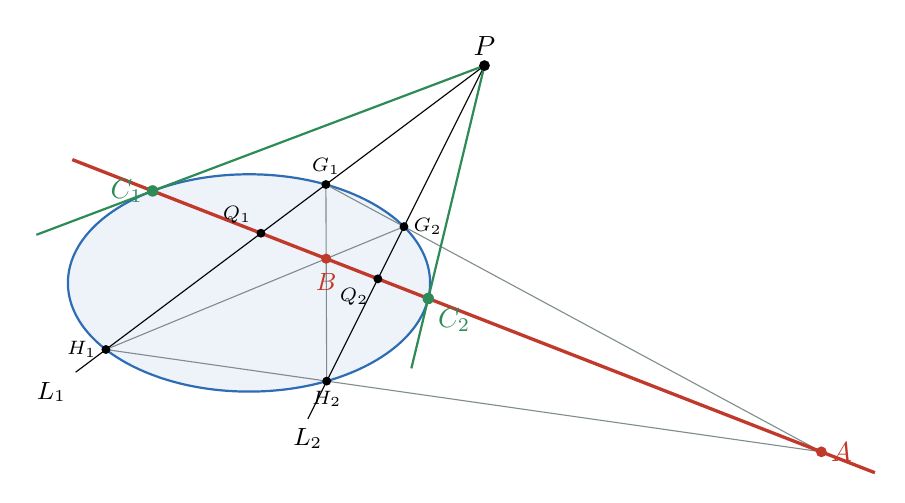
\begin{tikzpicture}[scale=1.15]
  \fill[defbg] (0,0) ellipse (2 and 1.2); \draw[thick,defblue] (0,0) ellipse (2 and 1.2);
  \coordinate (P) at (2.6,2.4); \coordinate (A) at (6.320,-1.865); \coordinate (B) at (0.852,0.268);
  \coordinate (G1) at (0.849,1.087); \coordinate (G2) at (1.711,0.622);
  \coordinate (H1) at (-1.580,-0.735); \coordinate (H2) at (0.858,-1.084);
  \coordinate (C1) at (-1.065,1.016); \coordinate (C2) at (1.979,-0.172);
  \coordinate (Q1) at (0.132,0.549); \coordinate (Q2) at (1.423,0.045);
  \draw (P)--($(P)!1.08!(H1)$) node[below left] {\small $L_1$}; \draw (P)--($(P)!1.12!(H2)$) node[below] {\small $L_2$};
  \draw[figgray] (G1)--(A) (H1)--(A);
  \draw[figgray] (H1)--(G2) (H2)--(G1);
  \draw[figred,very thick] ($(A)!-0.08!(C1)$)--($(A)!1.12!(C1)$);
  \draw[figgreen,thick] (P)--($(P)!1.35!(C1)$); \draw[figgreen,thick] (P)--($(P)!1.3!(C2)$);
  \foreach \p/\l/\pos in {G1/G_1/above,G2/G_2/right,H1/H_1/left,H2/H_2/below,Q1/Q_1/above left,Q2/Q_2/below left}{\fill (\p) circle (1.4pt) node[\pos] {\scriptsize $\l$};}
  \fill (P) circle (1.7pt) node[above] {$P$};
  \fill[keyred] (A) circle (1.7pt) node[right,keyred] {$A$};
  \fill[keyred] (B) circle (1.6pt) node[below=2pt,keyred] {\small $B$};
  \fill[figgreen] (C1) circle (1.8pt) node[left,figgreen] {$C_1$};
  \fill[figgreen] (C2) circle (1.8pt) node[below right,figgreen] {$C_2$};
\end{tikzpicture}
\caption{只用直尺作切线：$AB$ 是 $P$ 的极线（红），它交曲线于切点 $C_1,C_2$}
\end{figure}

\zheng 看内接于曲线的完备四点形 $G_1H_1G_2H_2$，它的三个对角点是
\[
G_1H_1\cap G_2H_2=L_1\cap L_2=P,\qquad G_1G_2\cap H_1H_2=A,\qquad H_1G_2\cap H_2G_1=B .
\]
由上面的“完备四点形调和性”，在边 $L_1=G_1H_1$ 上：$Q_1=L_1\cap AB$ 满足 $(G_1,H_1;P,Q_1)=-1$，即 $Q_1$ 是 $P$ 关于 $G_1,H_1$ 的第四调和点，所以 $Q_1$ 在 $P$ 的极线上；同理 $Q_2$ 也在。故 $AB=Q_1Q_2$ \key{就是 $P$ 的极线}。

$C_i$ 在 $P$ 的极线上，由配极原理 $P$ 在 $C_i$ 的极线上；而 $C_i$ 在曲线上，其极线就是 $C_i$ 处的切线。所以切线过 $P$，即 $PC_i$ 是切线。\qed

\begin{ex}{7.6.10$^*$}
怎样用直尺作过圆锥曲线上给定点的切线？
\end{ex}
\jie\textbf{方法一（用极线）}：设 $C$ 是曲线上的点。过 $C$ 作任一直线 $L_1$ 与曲线再交于 $D$；在 $L_1$ 上任取两点 $Q_1,Q_2$（不在曲线上），用第 9 题的方法分别作出它们的极线，设交于 $F$；则 $FC$ 就是过 $C$ 的切线。

\textbf{理由}：$F$ 在 $Q_1,Q_2$ 的极线上 $\Rightarrow$ $Q_1,Q_2$ 在 $F$ 的极线上 $\Rightarrow$ $F$ 的极线是 $Q_1Q_2=L_1$。$C\in L_1$ 是 $F$ 的极线上的点 $\Rightarrow$ $F$ 在 $C$ 的极线（即 $C$ 处的切线）上，所以切线是 $FC$。（$F$ 也在 $D$ 处的切线上：$F$ 是弦 $CD$ 的极点。）

\textbf{方法二（Pascal 的退化）}：在曲线上另取四点 $B,D,E,G$，对“六角形” $CCBDEG$（$CC$ 表示 $C$ 处的切线）用 Pascal 定理：$CB\cap EG=X$、$BD\cap GC=Y$ 两点确定 Pascal 线，它与 $DE$ 交于 $Z$，则 $CZ$ 是切线（切线 $CC$ 与对边 $DE$ 的交点也在 Pascal 线上）。

\begin{ex}{7.6.11$^*$}
对于非退化二次曲线 $\Sb$，给了一个配极映射 $\tau$，它把点 $P(x_1,x_2,x_3)\T$ 对应于点 $P$ 的极线 $L_P(\zeta_1,\zeta_2,\zeta_3)\T$，设 $\tau$ 的公式为
$\rho\begin{pmatrix}\zeta_1\\\zeta_2\\\zeta_3\end{pmatrix}=\begin{pmatrix}2&0&-1\\0&1&1\\-1&1&0\end{pmatrix}\begin{pmatrix}x_1\\x_2\\x_3\end{pmatrix}$。(1) 求直线 $L:\ x_1+x_2+x_3=0$ 的极点；(2) 求自共轭点的轨迹（若一个点 $P$ 的极线经过 $P$，则称 $P$ 是关于 $\Sb$ 的\key{自共轭点}）。
\end{ex}
\jie 配极映射的矩阵就是 $\Sb$ 的系数矩阵 $A$（极线坐标 $=A\vv p$）。

(1) 解 $A\vv p=\rho(1,1,1)\T$：
\[
\begin{cases}2p_1-p_3=\rho\\p_2+p_3=\rho\\-p_1+p_2=\rho\end{cases}\Rightarrow\ \vv p=\tfrac\rho3(1,4,-1)\T,
\]
极点为 $(1,4,-1)\T$。检验：$A(1,4,-1)\T=(3,3,3)\T$。\checkmark

(2) $P$ 自共轭 $\iff$ $L_P$ 过 $P$ $\iff$ $\zeta_1x_1+\zeta_2x_2+\zeta_3x_3=0\iff \rho^{-1}X\T AX=0$：
\[
2x_1^2+x_2^2-2x_1x_3+2x_2x_3=0 ,
\]
正是 $\Sb$ 本身——\key{配极映射决定了二次曲线}：曲线就是“在自己极线上”的点的轨迹。

\begin{ex}{7.6.12$^*$}
证明：如果一个完备四点形内接于一条二次曲线 $\Sb$，那么它的三对对边的交点形成一个自配极三角形。
\end{ex}
\zheng 设完备四点形 $ABCD$ 内接于 $\Sb$，对角点 $H=AB\cap CD$，$F=AC\cap BD$，$G=AD\cap BC$。

在边 $AC$ 上：由完备四点形的调和性，$F_1=AC\cap GH$ 满足 $(A,C;F,F_1)=-1$，而 $A,C\in\Sb$，所以 $F_1$ 在 $F$ 的极线上。同理在边 $BD$ 上，$F_2=BD\cap GH$ 满足 $(B,D;F,F_2)=-1$，$F_2$ 也在 $F$ 的极线上。$F_1\neq F_2$（$AC\neq BD$），所以 $F$ 的极线是 $F_1F_2=GH$。

同理 $G$ 的极线是 $FH$，$H$ 的极线是 $FG$。所以 $\triangle FGH$ 是自配极三角形。\qed

（第 9 题的图正是例子：内接四点形 $G_1H_1G_2H_2$ 的对角三角形 $PAB$ 是自配极的，$AB$ 是 $P$ 的极线。）

\begin{ex}{7.6.13$^*$}
证明：对于射影平面上任给一般位置的五个点（即其中任意三点不共线），有且只有一条二次曲线经过它们。
\end{ex}
\zheng\textbf{存在性}：二次曲线有 6 个系数（差一个倍数），过一点是关于系数的一个齐次线性方程。5 个方程、6 个未知量的齐次线性方程组必有非零解（\gd 未知量个数 $>$ 方程个数）。

\textbf{唯一性}：取基底使 $P_1=(1,0,0)\T,P_2=(0,1,0)\T,P_3=(0,0,1)\T,P_4=(1,1,1)\T$，设 $P_5=(p,q,r)\T$。过 $P_1,P_2,P_3$ 得 $a_{11}=a_{22}=a_{33}=0$，方程为 $a_{12}x_1x_2+a_{13}x_1x_3+a_{23}x_2x_3=0$；再过 $P_4,P_5$：
\[
\begin{cases}a_{12}+a_{13}+a_{23}=0,\\ pq\,a_{12}+pr\,a_{13}+qr\,a_{23}=0 .\end{cases}
\]
一般位置意味着 $P_5$ 不在 $P_iP_j$ 上：$p,q,r\neq0$（不在坐标三角形的边上），$p\neq q,\ q\neq r,\ r\neq p$（不在 $P_3P_4,P_1P_4,P_2P_4$ 上）。若系数矩阵 $\begin{psmallmatrix}1&1&1\\pq&pr&qr\end{psmallmatrix}$ 的秩为 1，则 $pq=pr=qr$，由 $p\neq0$ 得 $q=r$，矛盾。所以秩为 2，解空间 1 维，二次曲线唯一。\qed

\begin{intbox}{对照第 1 题}
第 1 题的五点中 $A,B,C$ 共线，不是一般位置，虽然二次曲线仍唯一，但它是退化的（两条直线）。若五点中有\key{四点}共线，则过它们的二次曲线就不唯一了（那条直线 + 过第五点的任一直线）。
\end{intbox}

% ================= 第七章总结 =================
\clearpage
\zongjie{第七章\ 总结}

\begin{center}
\renewcommand{\arraystretch}{1.35}
\begin{tabularx}{\linewidth}{@{}>{\raggedright\arraybackslash}p{2.3cm}>{\raggedright\arraybackslash}X>{\raggedright\arraybackslash}p{3.6cm}@{}}
\toprule
\textbf{\sffamily 内容} & \textbf{\sffamily 结论 / 方法} & \textbf{\sffamily 高代对应}\\\midrule
射影平面 & 欧氏平面 + 无穷远直线；任两线必交；点 $=\spn{\vv\alpha}$，线 $=\spn{\vv\beta,\vv\gamma}$ & 子空间格，维数公式\\
齐次坐标 & $(x,y)\to(x,y,1)$；方向 $(u,v)\to(u,v,0)$；差一个非零倍数 & 1 维子空间的生成元\\
连线 / 交点 & 都是叉积；三点共线 / 三线共点 $\iff$ 行列式 $=0$ & 线性相关；基础解系\\
对偶原理 & 点 $\leftrightarrow$ 线、共线 $\leftrightarrow$ 共点，定理成对出现 & 对偶空间 $V^*$\\
Desargues / Pappus & 证明都归结为 $\vv p+\vv q+\vv r=\vv0$ & 线性相关\\
交比 & $\dfrac{(c-a)(d-b)}{(c-b)(d-a)}=\dfrac{\lambda_2/\mu_2}{\lambda_1/\mu_1}$；24 种排列 6 个值 & $2\times2$ 行列式之比\\
调和 & $(A,B;C,D)=-1$；中点 $\leftrightarrow$ 无穷远点；完备四点形作图 & \\
射影坐标 & 基底 = 一般位置 4 点 $[A_1,A_2,A_3,E]$；变换 $\rho X=HX'$ & 基 + 单位点；过渡矩阵\\
射影变换 & $\lambda X'=AX$，$|A|\ne0$；4 对点唯一确定；保交比 & $PGL(3,\R)$，8 维\\
不动点 / 不变线 & $A$ 的特征向量 / $A\T$ 的特征向量；透射 $\sim\operatorname{diag}(e,1,1)$ & 特征值、可对角化\\
仿射变换 & = 保持 $l_\infty$ 的射影变换（第三行 $(0,0,1)$） & 子群\\
二次曲线 & $X\T AX=0$；与 $l_\infty$ 交 0/1/2 点 $\iff$ 椭圆/抛物线/双曲线 & 三元二次型\\
切线 / 极线 & $\vv p\T AX=0$；$(G,H;P,Q)=-1$；配极原理（对称性） & 对称双线性型，$A$-正交\\
中心、直径、准线 & 中心 = $l_\infty$ 的极点；直径 = 无穷远点的极线；准线 = 焦点的极线 & \\
自配极三角形 & 每边是对顶点的极线；内接四点形的对角三角形 & 合同对角化\\
射影分类 & 5 类：按秩与 $|$符号差$|$；椭圆、双曲线、抛物线同类 & 惯性定理\\
Steiner / Pascal & 曲线上看四定点交比为常数；内接六角形对边交点共线 & \\\bottomrule
\end{tabularx}
\end{center}

\begin{intbox}{全章一张图：几何 = 变换群 + 不变量}
\begin{center}
\renewcommand{\arraystretch}{1.25}
\begin{tabular}{@{}llll@{}}
\toprule
几何 & 变换（矩阵） & 典型不变量 & 二次曲线的分类数\\\midrule
欧氏 & 正交 $\begin{psmallmatrix}Q&\vv b\\0&1\end{psmallmatrix}$ & 距离、角度 & 无穷多（含 $a,b$ 等参数）\\
仿射 & $\begin{psmallmatrix}A_0&\vv b\\0&1\end{psmallmatrix}$ & 平行、分比 & 9 类（实）\\
射影 & 任意可逆 $A$（差倍数） & 共线、交比 & 5 类（实）\\\bottomrule
\end{tabular}
\end{center}
变换越多，能区分的图形越少：欧氏几何里大小不同的圆不同；仿射几何里所有椭圆相同；射影几何里椭圆、双曲线、抛物线都相同。
\end{intbox}

\begin{ckbox}{易错点清单}
\begin{enumerate}
\item 齐次坐标 $(0,0,0)$ 不代表任何点；坐标只确定到非零倍数，比较时看是否\key{成比例}。
\item 交比的“系数比”公式要先把 $C,D$ \key{同时}用 $A,B$ 表示；$C,D$ 的倍数可以乱取，但 $A,B$ 的向量在两次表示中必须是\key{同一组}。
\item 一般射影基底下，$x_3=0$ \key{不是}无穷远直线。
\item 求射影变换要 \key{4 对}一般位置点；只给 3 对点时答案含 2 个自由参数（习题 7.5.2）。
\item 点按 $A$ 变，线坐标按 $(A^{-1})\T$ 变（习题 7.5.3）；不变直线找 $A\T$ 的特征向量。
\item 过五点的二次曲线：先检查是否有三点共线（习题 7.6.1 的退化答案）。
\item 极线与切线同一个公式 $\vv p\T AX=0$，但 $P$ 在曲线外时它不是切线，而是切点弦。
\end{enumerate}
\end{ckbox}

\end{document}
